%% -*- coding: utf-8; fill-column: 150 -*-

\documentclass[a4paper,fontsize=11pt]{scrartcl}
\usepackage[utf8]{inputenc}
\usepackage{ngerman}
\usepackage{CJKutf8}
\usepackage{graphicx}
\usepackage{wrapfig}
\usepackage{fancyhdr}
\usepackage{amsfonts}
\usepackage{amsmath}
\usepackage{amssymb}
\usepackage{stmaryrd}
\usepackage{hyperref}
\usepackage{undertilde}
\usepackage{setspace}
\newenvironment{Japanese}{%  
\CJKfamily{min}%  
\CJKtilde  
\CJKnospace}{}
\pagestyle{fancy}
\usepackage{tikz}
\usetikzlibrary{arrows}% For nice arrow tips
% One style for all TikZ pictures for working with overlays:
\tikzset{every picture/.style=remember picture}
% Define a TikZ node for math content:
\newcommand{\mathnode}[2]{%
  \mathord{\tikz[baseline=(#1.base), inner sep = 0pt]{\node (#1) {$#2$};}}}

\DeclareMathOperator*{\bigdelta}{\Delta}
\newcommand{\simrightarrow}{\xrightarrow{\phantom{\sim}\sim\phantom{\sim}}}
\newcommand{\rng}{\operatorname{rng}}
\newcommand{\Term}{\operatorname{Term}}
\newcommand{\TC}{\operatorname{TC}}
\newcommand{\osharp}{\operatorname{O}^\sharp}
\newcommand{\ZFC}{\operatorname{ZFC}}
\newcommand{\ZF}{\operatorname{ZF}}
\newcommand{\GCH}{\operatorname{GCH}}
\newcommand{\Card}{\operatorname{Card}}
\newcommand{\Con}{\operatorname{Con}}
\newcommand{\Fml}{\operatorname{Fml}}
\newcommand{\On}{\operatorname{On}}
\newcommand{\cf}{\operatorname{cf}}
\newcommand{\otp}{\operatorname{otp}}
\newcommand{\dom}{\operatorname{dom}}
\newcommand{\id}{\operatorname{id}}
\newcommand{\height}{\operatorname{ht}}
\newcommand{\tp}{\operatorname{tp}}
\newcommand{\rn}{\operatorname{rn}}
\newcommand{\Hull}{\operatorname{Hull}}
\newcommand{\cp}{\operatorname{cp}}
\renewcommand{\bar}[1]{\overline{#1}} 
\renewcommand{\thefootnote}{[siehe \arabic{footnote}]}

\fancyhf{}
\fancyhead[L]{Große Kardinalzahlen}
\fancyhead[C]{}
\fancyhead[R]{\thepage}
\renewcommand{\headrulewidth}{0.4pt}
%%\author{Prof. Dr. H.-D. Donder}       %Authors
\begin{document}
\flushleft
\parskip1ex plus1ex minus0.5ex
\section*{Vorwort}
Fehler und Anmerkungen bitte an \textsc{christoph {\it punkt} senjak {\it at} ifi {\it punkt} lmu {\it punkt} de}.

{\bf Vorkenntnisse:} Logik, Modelle der Mengenlehre (Konstruktibles
Universum, Innere Modelle, kein Forcing)

{\bf Inhalt:} Ursprungliche Motivation für große Kardinalzahl-Axiome war, dass $\omega$ ein Sprung in den Kardinalzahlen ist. Man überlegte ob so ein
Sprungverhalten öfter vorkommen könnte. Die erste Vorgehensweise war, bestimmte Eigenschaften von $\omega$ zu isolieren, und dann eine Zahl mit den
gleichen Eigenschaften ungleich $\omega$ zu fordern. Dies ist allerdings inzwischen weitgehend obsolet.

Die Theorien die man durch große Kardinalzahlen bekommt ist eine Verstärkung der ursprünglichen Theorie. Man kann mit immer neuen großen
Kardinalzahlen immer neue Aussagen über natürliche Zahlen beweisen.

Das hier Behandelte ist im Wesentlichen die Einführung immer größerer Kardinalzahlen, relevant wird immer sein, ob man noch die natürlichen inneren
Modelle für große Kardinalzahlen hat.

{\bf Literatur:}
\begin{itemize}
  \item Drake, Set Theory - An Introduction To Large Cardinals
  \item Jech, Set Theory
  \item Kanamori, The Higher Infinite
\end{itemize}

{\bf Notation und Notizen:}
\begin{itemize}
  \item $[X]^n$ = Menge aller $n$-Elementigen Teilmengen von $X$
  \item $[X]^{<\omega} = \bigcup_n[X]^n$ = Menge aller endlichen
    Teilmengen von $X$
  \item gdw: genau dann wenn
  \item abg. unb.: abgeschlossen unbeschränkt
  \item $\otp$: Ordnungstyp
  \item $\overline{\cdot}$ ist {\bf kein} operator, sondern wird
    benutzt um zusätzliche Variablennamen zu generieren,
    $\overline{\kappa}$ hängt nicht mit $\kappa$ zusammen.
  \item $j:M\rightarrow_{\Sigma_\omega} N$: $j$ ist elementare
    Einbettung von $M$ in $N$
\end{itemize}

Wir betrachten oft Strukturen der Form
$\left<M,\in,A_1,\ldots,A_n\right>$ mit $A_i\subseteq M$.

{\bf Konvention:} Lasse das $\in$ weg, identifiziere
$\left<M,A_1,\ldots,A_n\right>$ mit
$\left<M,\in,A_1,\ldots,A_n\right>$.

{\bf Elementare Substruktur:} Sei
$\mathfrak{M}=\left<M,A_1,\ldots,A_n\right>$, $N\subseteq M$ und
$\mathfrak{N}=\left<N,A_1\cap N,\ldots,A_n\cap N\right>$ die
zugehörige Substruktur von $\mathfrak{M}$. Dann ist $\mathfrak{N}$
elementare Substruktur von $\mathfrak{M}$
(Bez. $\mathfrak{N}\prec\mathfrak{M}$ genau dann wenn für alle
$\varphi$ und $a_1,\ldots,a_k\in N$
$$ \mathfrak{M}\models \varphi[a_1,\ldots,a_k] \Leftrightarrow
\mathfrak{N}\models\varphi[a_1,\ldots,a_k]$$

{\bf Konvention:} Schreibe $N\prec\left<M,A_1,\ldots,A_n\right>$ statt
$\left<N,A_1\cap N,\ldots,A_n\cap
N\right>\prec\left<M,A_1,\ldots,A_n\right>$.

{\bf Skolemfunktionen:} Sei
$\mathfrak{M}=\left<M,\in,A_1,\ldots,A_n\right>$ eine
${\mathcal{L}}$-Struktur. Für eine $\mathcal{L}$-Formel
$\varphi(\vec{x},y)$ definiere $f_\varphi$ so, dass gilt

$$ \mathfrak{M}\models \exists_y \varphi[\vec{a},y] \Rightarrow
\mathfrak{M}\models\varphi[\vec{a},f_\varphi(\vec{a})]$$

Setze
$\mathcal{F}=\{f_\varphi\mid\varphi\phantom{a}\mathcal{L}-\mbox{Formel}\}$. Dann
gilt:

Sei $N\subseteq M$, $N\neq\emptyset$, unter allen $f\in\mathcal{F}$
abgeschlossen (d.h. $\vec{a}\in N,f\in\mathcal{F}\Rightarrow
f(\vec{a})\in N$). Dann ist $N\prec\mathfrak{M}$.

\underline{Wir sagen:} $\mathcal{F}$ ist Menge von Skolemfunktionen
für $\mathfrak{M}$. Beachte, dass $\mathcal{F}$ abzählbar ist.

\section{``Kleine'' große Kardinalzahlen}
Arbeite in ZFC. Wir nehmen an, dass ZFC widerspruchsfrei ist.

{\bf Definition:} $\kappa$ ist (stark) unerreichbar $\Leftrightarrow$
$\kappa>\omega$, $\kappa$ regulär und für alle $\lambda<\kappa$ gilt
$2^\lambda<\kappa$.

{\bf Bemerkung:} $\omega$ ist regulär und für alle $n<\omega$ ist
$2^n<\omega$.

{\bf Lemma 1:} Sei $\kappa$ unerreichbar. Dann gilt für alle
$\alpha<\kappa$ dass $|V_\alpha|<\kappa$ (also $|V_\kappa|=\kappa$).

{\bf Beweis:} Durch Induktion über $\alpha<\kappa$:
\begin{itemize}
  \item $\alpha=0$: $V_0=\emptyset$. Also $|V_0|=0<\kappa$.
  \item $\alpha=\beta+1$: $V_{\beta+1}=\mathfrak{P}(V_\beta)$. Also
    $|V_{\beta+1}|=2^{|V_\beta|}$. Nach Induktion ist
    $|V_\beta|<\kappa$. Also nach Definition $2^{|V_\beta|}<\kappa$.
  \item $\lim(\lambda)$: Es ist
    $V_\lambda=\bigcup\limits_{\alpha<\lambda} V_\alpha$. Also
    $|V_\lambda|\le |\lambda|\cdot
    \sup\{|V_\alpha|\mid\alpha<\lambda\}$. Wegen $\lambda<\kappa$ genügt
    es also zu zeigen, dass
    $\sup\{|V_\alpha|\mid\alpha<\lambda\}<\kappa$. Also für
    $\alpha<\lambda$ ist $|V_\alpha|<\kappa$ nach
    Induktionsvoraussetzung und $\lambda<\kappa$. Wegen $\kappa$
    regulär ist also $\sup\{|V_\alpha|\mid\alpha<\lambda\}<\kappa$.
\end{itemize}
\hfill $\square$

{\bf Lemma 2:} Sei $\kappa$ unerreichbar und $u\subseteq
V_\kappa$. Dann gilt $u\in V_\kappa\Leftrightarrow|u|<\kappa$.

{\bf Beweis:}
\begin{itemize}
\item[$\rightarrow$:] Sei $u\in V_\kappa$. Dann existiert
  $\alpha<\kappa$ mit $u\in V_\alpha$. Wegen $V_\alpha$ transitiv also
  $u\subseteq V_\alpha$. Somit $|u|\le|V_\alpha|
  \stackrel{\mbox{\tiny L1}}{<} \kappa$.
\item[$\leftarrow$:] Sei $|u|<\kappa$. Definiere $g:u\rightarrow \On$
  durch $g(x)=\min\{\alpha\mid x\in V_\alpha\}$. Wegen $u\subseteq V_k$
  ist $\rng(g)\subseteq\kappa$. Aber $|\rng(g)|\le |u|<\kappa$. Wegen
  $\kappa$ regulär ist also $\rng(g)$ beschränkt in $\kappa$. Sei
  $\gamma=\sup \rng (g)$. Dann ist $u\subseteq V_\gamma$, denn für
  $x\in u$ ist $x\in V_{g(x)}\subseteq V_\gamma$. Also $u\in
  V_{\gamma+1}\subseteq V_\kappa$.
\end{itemize}
\hfill $\square$

{\bf Satz 3:} Sei $\kappa$ unerreichbar. Dann $V_\kappa\models ZFC$.

{\bf Beweis:}
\begin{itemize}
\item (Ext) und (Fund) sind $\Pi_1$. Sie gelten also in $V_\kappa$, da
  $V_\kappa$ transitiv.
\item (Null) da $\emptyset\in V_\kappa$.
\item (Un) da $\omega=\On\cap V_\omega \in V_{\omega+1}\subseteq
  V_\kappa$ (da $\kappa>\omega$).
\item (Paar) Seien $x,y\in V_\kappa$. Dann existieren
  $\alpha,\beta<\kappa$ mit $x\in V_\alpha$ und $y\in V_\beta$. Setze
  $\gamma=\max\{\alpha,\beta\}$. Also $\{x,y\}\subseteq V_\gamma$ und
  somit $\{x,y\}\in V_{\gamma+1}\subseteq V_\kappa$.
\item (Ver) Sei $x\in V_\kappa$. Dann existiert $\alpha<\kappa$ mit
  $x\in V_\alpha$. Also wegen $V_\alpha$ transitiv $\bigcup x\subseteq
  V_\alpha$. Somit $\bigcup x\in V_{\alpha+1}\subseteq V_\kappa$.
\item (Pot) Sei $x\in V_\kappa$. Dann existiert $\alpha<\kappa$ mit
  $x\in V_\alpha$. Also $x\subseteq V_\alpha$ und daher
  $\mathfrak{P}(x)\subseteq\mathfrak{P}(V_\alpha)=V_{\alpha+1}$. Somit
  $\mathfrak{P}(X)\in V_{\alpha+2}\subseteq V_\kappa$.
\item (Ers) Es genügt folgendes zu zeigen: Sei $F:A\rightarrow
  V_\kappa$ Funktion mit $A\subseteq V_\kappa$ und sei $u\in
  V_\kappa$. Dann ist $F''u\in V_\kappa$. Sei also $F:A\rightarrow
  V_\kappa$ gegeben und $u\in V_\kappa$. Dann ist auch $u\subseteq
  V_\kappa$ und nach Lemma 2 $|u|<\kappa$. Setze $v=F''u$. Also
  $v\subseteq V_\kappa$ und $|v|\le |u|<\kappa$. Somit nach Lemma 2
  $v\in V_\kappa$.
\item (AC) Sei $u\in V_\kappa$ mit $\emptyset\not\in u$. Sei $f$ eine
  Auswahlfunktion für $u$. Also ist $f\subseteq u\times\bigcup u$. Sei
  $\alpha<\kappa$ mit $u\in V_\alpha$. Dann ist aber $u\times\bigcup
  u\subseteq V_\alpha\times V_\alpha\subseteq V_{\alpha+2}$. Also
  $f\in V_{\alpha+3}\subseteq V_\kappa$.
\end{itemize}
\hfill $\square$

{\bf Folgerung:} $\ZFC + \exists_\kappa \kappa\mbox{ unerreichbar
}\vdash \Con(\ZFC)$. Also nach Gödel
$\ZFC\not\vdash\exists_\kappa\kappa\mbox{ unerreichbar}$. Sogar ohne
Gödel, denn:

{\bf Annahme:} $\ZFC\vdash\exists_\kappa\kappa\mbox{
  unerreichbar}$. Sei $\kappa$ die kleinste unerreichbare
Kardinalzahl. Dann $V_\kappa\models\ZFC+\mbox{existiert keine
  unerreichbare Kardinalzahl}$. Widerspruch.


%% ========= EINGEFÜGT ===============


{\bf Satz 4:} Es sind äquivalent
\begin{itemize}
\item[(1)] $\kappa$ ist unerreichbar
\item[(2)] Für alle $A\subseteq V_{\kappa}$ ist $\{\alpha <\kappa \mid
  V_{\alpha} \prec \langle V_{\kappa}, A\rangle\}$ abgeschlossen und
  unbeschränkt in $\kappa$
\item[(3)] Für alle $A\subseteq V_{\kappa}$ und (erststufigen) $\varphi$
  mit $\langle V_{\kappa}, A\rangle\models \varphi$ existiert
  $\alpha<\kappa$ mit $\langle V_{\alpha}, A\cap V_{\alpha} \rangle
  \models \varphi$
\end{itemize}

{\bf Beweis:}
\begin{itemize}
\item (1)$\Rightarrow$(2): Sei $A\subseteq V_{\kappa}$. Setze $C=\{\alpha<\kappa\mid V_{\alpha}\prec \langle V_{\kappa}, A\rangle\}$.
  \begin{itemize}
  \item[(a)] $C\mbox{ ist abgeschlossen in }\kappa$: Sei $\alpha <
    \kappa$ ein Limespunkt von $C$.  Dann ist $V_{\alpha} =
    \bigcup_{\gamma\in C\cap\alpha} V_{\gamma}$.  Also $V_{\alpha}
    \prec \langle V_{\kappa}, A\rangle$ nach dem Lemma von Tarski über
    elementare Ketten.
  \item[(b)] $C\mbox{ ist unbeschränkt in }\kappa$: Sei $\mathcal F$
    eine Menge von Skolemfunktionen für $\langle V_{\kappa},
    A\rangle$.  Für $f\in \mathcal F$ sei $C_f = \{\alpha<\kappa\mid
    f''V_{\alpha}^{\kappa_f} \subseteq V_{\alpha}\}$.
  \item[(c)] $C_f\mbox{ ist abeschlossen und unbeschränkt in }\kappa$:
    Abgeschlossenheit ist klar.  Zur Unbeschränktheit: Sei
    $\alpha<\kappa$.  Definiere rekursiv die monotone Folge
    $\alpha_0<\alpha_1<\cdots<\kappa$ wie folgt: Setze
    $\alpha_0=\alpha$.  Im $n$-ten Schritt $v_n=
    f''V_{\alpha_n}^{\kappa_f}$.  Dann wegen $\kappa$ unerreichbar
    $|v_n|<\kappa$.  Also ist $v_n\in V_{\kappa}$ nach Lemma 2.  Also
    existiert $\beta>\alpha_n$ mit $\beta<\kappa$ und $v_n\subseteq
    V_{\beta}$.  Setze $\alpha_{n+1}=\beta$.  Dann gilt also
    $f''V_{\alpha_n}^{n_f}\subseteq V_{\alpha_{n+1}}$.  Sei dann
    $\gamma = \sup_n \alpha_n$.  Dann $\gamma <\kappa$, da
    $\cf(\kappa)>\kappa$ und natürlich $\gamma >\alpha$.  Aber
    $\gamma\in C_f$, da
    $f''V_{\gamma}^{n_f}=\bigcup_{n\in\omega}f''V_{\alpha}^{n_f}
    \subseteq \bigcup_{n\in\omega}V_{\alpha_{n+1}} = V_{\gamma}$.
  \end{itemize}
  Setze nun $D=\bigcup_{f\in \mathcal F} C_f$.  Wegen $\mathcal F$
  abzählbar ist $D$ nach $(c)$ abg. unb. in $\kappa$.  Aber
  $D\subseteq C$, dann ist $\alpha\in D$, so für alle $f\in \mathcal
  F$: $f''V^{\kappa_f}_{\alpha}\subseteq V_{\alpha}$, also
  $V_{\alpha}\prec \langle V_{\kappa}, A\rangle$.
\item (2)$\Rightarrow$(3): Trivial.
\item (3)$\Rightarrow$(1): Sei (3) erfüllt.
  \begin{itemize}
  \item[(i)] $\kappa\mbox{ ist Limesordinalzahl}$: Offenbar
    $\kappa\neq 0$.  $\lightning$-Annahme: $\kappa=\gamma+1$.  Setze
    $A=\{\gamma\}$.  Dann $\langle V_{\kappa},A\rangle\models
    A\neq\emptyset$ (genau: $\langle V_{\kappa},A\rangle\models
    \exists x\; A(x)$). Wähle nach (3) ein $\alpha<\kappa$ mit
    $\langle V_{\alpha}, A\cap V_{\alpha}\rangle\models A\neq
    \emptyset$.  Dann aber $\gamma \in A\cap V_{\alpha}$, d.h. $\gamma
    \in V_{\alpha}$, also $\gamma<\alpha$.  $\lightning$ zu
    $\alpha<\kappa=\gamma+1$.
  \item[(ii)] $\kappa>\omega$: $\lightning$-Ann.: $\kappa<\omega$.
    Dann nach $(i)$ $\kappa=\omega$.  Aber
    $(V_{\omega}\models\forall\gamma\in\On\; \exists \delta\in\On\;
    \gamma<\delta)\land \exists x\; x=x$ %underbrace \varphi und für
    alle $n<\omega$: $V_n\models \neg\varphi$.  $\lightning$ zu (3).
  \item[(iii)] $\kappa\mbox{ ist regulär}$: Sei $\gamma<\kappa$ und
    $f\colon\gamma\to\kappa$.  Wir müssen zeigen, dass $f$ beschränkt
    in $\kappa$ ist.  Wir können o.E. annehmen, dass $f(0)=\gamma$.
    Setze $A=f\subseteq V_{\kappa}$.  Dann \[\langle
    V_{\kappa},A\rangle\models \mbox{''$A$ ist Funktion, dann
      $(A)=A(0)$''}\] Gemäß (3) wähle $\alpha<\kappa$ mit $\langle
    V_{\alpha}, A\cap V_{\alpha}\models \varphi$.  Setze $g=A\cap
    V_{\alpha}$.  Dann $0\in\dom(g)$.  Also $g(0)=f(0)=\gamma \in
    V_{\alpha}$.  Außerdem $dom(g)=g(0)=\gamma$.  Also $g=f$,
    d.h. $f\subseteq V_{\alpha}$ und damit $\rng(f)\subseteq On\cap
    V_{\alpha}=\alpha$.  Also $f$ beschränkt in $\kappa$.
  \item[(iv)] $\mbox{für alle} \lambda<\kappa \; 2^{\lambda}<\kappa$:
    Sei $\lambda<\kappa$ und $f\colon \mathfrak P(\lambda)\to\kappa$.
    Wir müssen zeigen, dass $f$ nicht surjektiv ist.  Sei
    o.E. $f(\emptyset)=\lambda$.  Setze $A=f\subseteq V_{\kappa}$.
    Dann $\langle V_{\kappa}, A\rangle\models \mbox{''$A$ ist
      Funktion, $\dom(A)=\mathfrak(A(\emptyset))$''}$.  Gemäß (3)
    wähle $\alpha<\kappa$ mit $\langle V_{\alpha}, A\cap
    V_{\alpha}\rangle\models\varphi$.  Setze $g=A\cap V_{\alpha}$.
    Dann $\emptyset\in\dom(g)$.  Also
    $g(\emptyset)=f(\emptyset)=\lambda\in V_{\alpha}$.  Außerdem
    $\dom(g)=\mathfrak P(g(\emptyset)) = \mathfrak P(\lambda)$.  Also
    $g=f$, d.h. $f\subseteq V_{\alpha}$ und somit
    z.B. $\alpha\not\in\rng(f)$
  \end{itemize}
\end{itemize}
\hfill $\square$

{\bf Lemma 5:} Sei $W$ ein inneres Modell. Sei $\kappa$
unerreichbar. Dann ist $\kappa$ unerreichbar in $W$.

{\bf Beweis:} $\kappa$ ist regulär in $W$, denn Regularität ist eine
$\Pi_1$-Eigenschaft. Sei $\lambda<\kappa$. Dann $(2^{\lambda})^W\le
2^{\lambda}<\kappa$.

\hfill $\square$

{\bf Definition:} $\kappa$ ist \emph{schwach unerreichbar} $\iff$
$\kappa>\omega$ und $\kappa$ ist reguläre Limesordinalzahl.

{\bf Anmerkung:} Sei $W$ ein inneres Modell. Sei $\kappa$ schwach
unerreichbar. Dann ist $\kappa$ schwach unerreichbar in $W$.

{\bf Anmerkung:} Sei $\kappa$ schwach unerreichbar. Dann ist $\kappa$ unerreichbar in $L$.

{\bf Beweis:} $\kappa$ ist schwach unerreichbar in $L$. Aber $L\models
GCH$. Also ist $\kappa$ unerreichbar in $L$.

\hfill $\square$

Wir können z.B. definieren: $\kappa$ ist \emph{hyperunerreichbar}
$\iff$ $\kappa$ ist unerreichbar und $\kappa
=\sup\{\tau<\kappa\mid\tau \mbox{ unerreichbar}\}$. Das lässt sich
beliebig weitertreiben: hyperhyperunerreichbar,
hyperhyperhyperunerreichbar usw...

{\bf Definition:} $\kappa$ ist \emph{Mahlo} $\iff$ $\kappa$ ist
unerreichbar und $\{\tau<\kappa\mid \tau \mbox{ ist regulär}\}$ ist
stationär in $\kappa$.

{\bf Bemerkung:} $\kappa$ Mahlo $\Rightarrow$ $\{ \tau<\kappa\mid \tau\mbox{ unerreichbar}\}$ ist stationär in $\kappa$.

{\bf Beweis:} Sei $\kappa$ Mahlo. Sei $E= \{\tau<\kappa\mid \tau
\mbox{ regulär} \}$. Setze $$C=\{ \tau<\kappa\mid \tau>\omega \mbox{
  und für alle }\lambda<\tau\; 2^{\lambda}<\tau\}$$ $C$ ist
abg. unb. in $\kappa$, denn: Abg. ist klar.  Unb.: Sei
$\alpha<\kappa$.  Setze $\tau_0=\max\{\alpha,\omega\}$,
$\tau_{n+1}=2^{\tau_n}$.  Wegen $\kappa$ unerreichbar ist
$\tau_n<\kappa$.  Setze $\tau=\sup_n\tau_n$.  Dann auch $\tau<\kappa$
und $\tau\in C$.  Wegen $\kappa$ Mahlo ist $E$ stationär in $\kappa$.
Also ist $\{\tau<\kappa\mid \tau\mbox{ unerreichbar }\} = C\cap E$
stationär in $\kappa$.

\hfill $\square$

{\bf Lemma 6:} Sei $\kappa$ Mahlo. Dann gilt: 
\begin{itemize}
\item[(a)] $\kappa$ ist hyperunerreichbar
\item[(b)] $\{\tau<\kappa\mid \tau \mbox{ ist hyperunerreichbar}\}$ ist stationär in $\kappa$.
\end{itemize}

{\bf Beweis:}
\begin{itemize}
\item[(a)] Ist klar, da nach Bemerkung $\{\tau<\kappa\mid \tau\mbox{ unerreichbar}\}$  sogar stationär in $\kappa$, also auch unbeschränkt in $\kappa$.
\item[(b)] Sei $A=\{\tau<\kappa\mid \tau \mbox{ unerreichbar}\}$. Nach
  (a) ist $A$ unbeschränkt in $\kappa$. Also ist $C=\{ \tau<\kappa\mid
  \tau=\sup(A\cap\tau)\}$ abg. unb. in $\kappa$. Da $A$ sogar
  stationär in $\kappa$, ist also $\{\tau<\kappa\mid \kappa \mbox{ ist
    hyperunerreichbar}\}=C\cap A$ stationär in $\kappa$.
\end{itemize}

\hfill $\square$

%% ========= /EINGEFÜGT ===============

{\bf 1. Übung:}

{\bf Aufgabe 1:} Sei $\kappa\in\On$. Zeigen Sie, dass folgende
Aussagen äquivalent sind:
\begin{enumerate}
\item $\kappa$ ist unerreichbar
\item für alle $f:V_\kappa\rightarrow\kappa$ existiert
  $0<\alpha<\kappa$ mit $f''V_\alpha\subseteq\alpha$
\end{enumerate}

{\bf Aufgabe 2:} Seien $\alpha,\beta\in\On$ mit $\alpha<\beta$, und es
gelte $V_\alpha\prec V_\beta$. Zeigen Sie, dass $V_\alpha\models\ZFC$.

{\bf Satz 7:} Es sind äquivalent
\begin{itemize}
  \item[(1)] $\kappa$ ist Mahlo
  \item[(2)] für alle $A\subseteq V_\kappa$ existiert ein reguläres
    $\alpha<\kappa$ mit $V_\alpha\prec\left<V_\kappa,A\right>$
  \item[(3)] für alle $A\subseteq V_\kappa$ mit
    $\left<V_\kappa,A\right>\models\varphi$ ($\varphi$ erststufig)
    existiert ein reguläres $\alpha<\kappa$ mit $\left<V_\alpha,A\cap
    V_\alpha\right>\models\varphi$
\end{itemize}

{\bf Beweis:}
\begin{itemize}
\item (1)$\Rightarrow$(2): Sei $\kappa$ Mahlo. Sei $A\subseteq
  V_\kappa$. Wegen $\kappa$ unerreichbar ist dann nach Satz 4
  $C=\{\alpha<\kappa\mid V_\alpha\prec\left<V_\kappa,A\right>\}$
    abgeschlossen unbeschränkt in $\kappa$. Wegen $\kappa$ Mahlo
    existiert also $\alpha\in C$ mit $\alpha$ regulär.
\item (2)$\Rightarrow$(3): Trivial.
\item (3)$\Rightarrow$(1): Sei (3) erfüllt. Dann ist $\kappa$
  unerreichbar nach Satz 4. Sei $E=\{\alpha<\kappa\mid \alpha\mbox{
    regulär}\}$. Noch zu zeigen, dass $E$ stationär in $\kappa$. Sei
  hierzu $C\subseteq\kappa$ abgeschlossen unbeschränkt in
  $\kappa$. Dann
  $\left<V_\kappa,C\right>\models\underbrace{\forall_{\gamma\in\On}\exists_{\delta\in
      C}\gamma<\delta}_\varphi$. Gemäß (3) wähle ein reguläres
  $\alpha<\kappa$ mit $\left<V_\alpha,C\cap
  V_\alpha\right>\models\varphi$. Nun ist $C\cap V_\alpha=C\cap\alpha$
  da $C\subseteq\On$ und $V_\alpha\cap\On=\alpha$. Somit ist
  $C\cap\alpha$ unbeschränkt in $\alpha$. Also ist $\alpha\in C$, da
  $C$ abgeschlossen in $\kappa$. Wegen $\alpha$ regulär ist $C\cap
  E\neq\emptyset$.
\end{itemize}
\hfill $\square$

{\bf Lemma 8:} Sei $W$ ein inneres Modell von $\ZFC$. Sei $\kappa$
Mahlo. Dann ist $\kappa$ Mahlo in $W$.

{\bf Beweis:} Nach Lemma 5 ist $\kappa$ unerreichbar in $W$. Sei $C\in
W$ abgeschlossen unbeschränkt in $\kappa$. Dann existiert $\alpha\in
C$ mit $\alpha$ regulär. Dann ist aber $\alpha$ auch regulär in
$W$. Somit ist $\{\alpha<\kappa\mid \alpha\mbox{ regulär in }W\}$
stationär in $\kappa$ (in $W$).

\hfill $\square$

Wir können die Definition von Mahlo ``iterieren'', zum Beispiel

{\bf Definition:} $\kappa$ ist $2$-Mahlo $:\Leftrightarrow$ $\kappa$
ist unerreichbar und $\{\alpha<\kappa\mid \alpha\mbox{ Mahlo}\}$ ist
stationär in $\kappa$.

{\bf Bemerkung:} $\kappa$ ist $2$-Mahlo $\Rightarrow$ $\kappa$ Mahlo.

{\bf Satz 9:} Es sind äquivalent:
\begin{itemize}
\item[(1)] $\kappa$ ist $2$-Mahlo
\item[(2)] für alle $A\subseteq V_\kappa$ existiert Mahlo
  $\alpha<\kappa$ mit $V_\alpha\prec\left<V_\kappa,A\right>$
\item[(3)] für alle $A\subseteq V_\kappa$ mit
  $\left<V_\kappa,A\right>\models\varphi$ ($\varphi$ erststufig)
  existiert Mahlo $\alpha<\kappa$ mit $\left<V_\alpha,A\cap
  V_\alpha\right>\models\varphi$
\end{itemize}
{\bf Beweis:} Völlig analog zu Beweis von Satz 7.

\hfill $\square$

Noch größere Kardinalzahlen erhalten wir, wenn wir die Eigenschaft (3)
aus Satz 4 ``für alle $A\subseteq V_\kappa$ und erststufigen $\varphi$
mit $\left<V_\kappa,A\right>\models\varphi$ existiert ein
$\alpha<\kappa$ mit $\left<V_\alpha,A\cap
V_\alpha\right>\models\varphi$'' wesentlich verstärken.

{\bf Definition:} $\kappa$ ist schwach kompakt
(bzw. $\Pi_1^1$-unbeschreibbar wenn folgendes gilt:

Sei $A\subseteq V_\kappa$ und es gelte für alle $B\subseteq V_\kappa$
dass $\left<V_\kappa, A, B\right>\models\varphi$ ($\varphi$
erststufig). Dann existiert $\alpha<\kappa$ mit für alle $B\subseteq
V_\alpha$ $\left<V_\alpha,A\cap V_\alpha,B\right>\models\varphi$.

{\bf Definition:} Sei $Q$ eine Eigenschaft von Ordinalzahlen. Wir
sagen $Q$ ist eine $\Pi_1^1$-Eigenschaft, wenn existiert erststufiges
$\varphi$ mit $Q(\kappa)$ $\Leftrightarrow$ für alle $B\subseteq
V_\kappa$ gilt $\left<V_\kappa,B\right>\models\varphi$.

{\bf Bemerkung:} Sei $Q$ eine $\Pi_1^1$-Eigenschaft. Sei $\kappa$
schwach kompakt. Weiterhin gelte $Q(\kappa)$. Dann existiert ein
$\tau<\kappa$ mit $Q(\tau)$. ``$\kappa$ ist schwach kompakt'' ist also
keine $\Pi_1^1$-Eigenschaft. Die bisherigen Eigenschaften sind aber
$\Pi_1^1$-Eigenschaften.

{\bf Lemma 10:} ``$\kappa$ ist regulär'', ``$\kappa$ ist
unerreichbar'', ``$\kappa$ ist Mahlo'', ``$\kappa$ ist $2$-Mahlo''
sind $\Pi_1^1$-Eigenschaften.

{\bf Beweis:} Nehme einfach die üblichen Definitionen.

\hfill $\square$

{\bf Satz 11:}
\begin{itemize}
\item[(a)] $\kappa$ schwach kompakt $\Rightarrow$ $\kappa$ ist
  $2$-Mahlo
\item[(b)] $\kappa$ schwach kompakt $\Rightarrow$ existiert
  $\tau<\kappa$ mit $\tau$ ist $2$-Mahlo
\end{itemize}

{\bf Beweis:}
\begin{itemize}
\item[(a)] Sei $\kappa$ schwach kompakt. Nach Definition ist dann die
  Bedingung (3) aus Satz 4 erfüllt. Also ist $\kappa$
  unerreichbar. Wir zeigen zuerst, dass $\kappa$ Mahlo ist. Hierzu
  zeigen wir die Bedingung (3) aus Satz 7. Sei also $A\subseteq
  V_\kappa$ mit $\left<V_\kappa,A\right>\models\varphi$ ($\varphi$
  erststufig). Zu zeigen ist, es existiert ein reguläres
  $\alpha<\kappa$ mit $\left<V_\alpha,A\cap
  V_\alpha\right>\models\varphi$. Nach Lemma 10 sei $\psi$ erststufig
  mit:
  $$ \tau\mbox{ ist regulär}\Leftrightarrow\mbox{für alle }B\subseteq
  V_\kappa\left<V_\kappa,B\right>\models\psi$$
  Da ja $\kappa$ regulär ist, gilt dann:
  $$ \mbox{für alle }B\subseteq
  V_\kappa\phantom{a}\left<V_\kappa,A,B\right>\models\varphi\wedge\psi$$
  Also wegen $\kappa$ schwach kompakt existiert $\alpha<\kappa$ mit
  $$ \mbox{für alle }B\subseteq
  V_\alpha\phantom{a}\left<V_\alpha,A\cap
  V_\alpha,B\right>\models\varphi\wedge\psi$$ Also ist $\alpha$
  regulär und $\left<V_\alpha,A\cap V_\alpha\right>\models\varphi$,
  was zu zeigen war. Nun wissen wir, dass $\kappa$ Mahlo ist. Nun ist
  aber nach Lemma 10 auch die Eigenschaft ``$\tau$ ist Mahlo'' eine
  $\Pi_1^1$-Eigenschaft. Also können wir völlig Analog die Eigenschaft
  (3) aus Satz 9 zeigen. Somit ist $\kappa$ $2$-Mahlo.
\item[(b)] Nach Lemma 10 ist auch die Eigenschaft ``$\tau$ ist
  2-Mahlo'' eine $\Pi_1^1$-Eigenschaft. Also folgt die Behauptung aus
  (a) und Bemerkung.
\end{itemize}

\hfill $\square$

{\bf Lemma 12:} Sei $\kappa$ schwach kompakt. Seien
$A_1,\ldots,A_n\subseteq V_\kappa$, $\varphi$ erststufig, und es
gelte: Für alle $B\subseteq V_\kappa$ haben wir
$\left<V_\kappa,A_1,\ldots,A_n,B\right>\models\varphi$. Dann existiert
ein $\alpha<\kappa$ mit für alle $B\subseteq V_\alpha$ gilt
$\left<V_\alpha,A_1\cap V_\alpha,\ldots,A_n\cap
V_\alpha,B\right>\models\varphi$.

{\bf Beweisskizze:} Setze $A=\bigcup_{i=1}^{n}\{i\}\times A_i$. dann
ist $A_i$ kanonisch definierbar in $\left<V_\kappa,A\right>$ durch
$A_i=\{x\mid\left<i,x\right>\in A\}$. Übersetze hiermit $\varphi$ in
$\varphi^x$. Wähle $\alpha<\kappa$ mit für alle $B\subseteq
V_\alpha\phantom{a}\left<V_\alpha,A\cap
V_\alpha,B\right>\models\varphi^x \wedge
\forall_{\gamma\in\On}\exists_{\delta\in\On}\gamma\in\delta$. Dann ist
$\alpha$ Limesordinalzahl, also $A_i\cap
V_\alpha=\{x\mid\left<i,x\right>\in A\cap V_\alpha\}$. Durch
Rückübersetzung also für alle $B\subseteq V_\alpha$
$\left<V_\alpha,A_1\cap V_\alpha,\ldots,A_n\cap
V_\alpha,B\right>\models\varphi$

\hfill $\square$

{\bf Lemma 13:} Sei $\kappa$ schwach kompakt. Sei
$A_1,\ldots,A_n\subseteq V_\kappa$, $\varphi$ erststufig, und es
gelte: für alle $B\subseteq V_\kappa$ ist
$\left<V_\kappa,A_1,\ldots,A_n,B\right>\models\varphi$. Setze
$E=\{\alpha<\kappa\mid\mbox{für alle }B\subseteq V_\alpha\mbox{ gilt
}\left<V_\alpha,A_1\cap V_\alpha,\ldots,A_n\cap V_\alpha,
B\right>\models\varphi\}$. Dann ist $E$ stationär in $\kappa$.

{\bf Beweis:} Sei $C\subseteq\kappa$ abgeschlossen unbeschränkt in
$\kappa$. Zu zeigen $E\cap C\neq\emptyset$. Nun aber: für alle
$B\subseteq V_\kappa$
$\left<V_\kappa,A_1,\ldots,A_n,C,B\right>\models\underbrace{\varphi\wedge\forall_{\gamma\in\On}\exists_{\delta\in
    C}\gamma<\delta}_\psi$. Also nach Lemma 12 existiert
$\alpha<\kappa$ mit: für alle $B\subseteq
V_\alpha\phantom{a}\left<V_\alpha,A_1\cap V_\alpha,\ldots,A_n\cap
V_\alpha,C\cap V_\alpha, B\right>\models\psi$. Dann natürlich
$\alpha\in E$. Aber auch $\sup(C\cap\alpha)=\alpha$. Also $\alpha\in
C$, da $C$ abgeschlossen in $\kappa$.

\hfill $\square$

{\bf Definition:} Sei $f:[z]^n\rightarrow\gamma$ eine Partition von
$[z]^n$. $x\subseteq z$ heißt {\it homogen} für $f$ genau dann wenn
$\exists_{\beta<\gamma} f''[x]^n\subseteq\{\beta\}$.
$$ \kappa \rightarrow (\delta)_\gamma^n \Leftrightarrow \mbox{für alle
} f:[\kappa]^n\rightarrow\gamma\mbox{ existiert
}X\subseteq\kappa\mbox{ homogen für }f\mbox{ mit }\otp(X)=\delta $$

{\bf Bemerkung:} Falls $\kappa\rightarrow(\delta)_\gamma^n$ und
$\overline{\kappa}\ge\kappa,\lim(\kappa),\overline{\delta}\le\delta,\overline{\kappa}\le\kappa$,
so
$\overline{\kappa}\rightarrow(\overline{\delta})_{\overline{\gamma}}^{\overline{n}}$.

{\bf Wiederholung:}
Folgende Begriffe werden als bekannt vorausgesetzt:
\begin{itemize}
\item Ein {\it Baum} ist eine partiell geordnete Menge, sodass die
  Vorgänger jedes Elementes wohlgeordnet sind. Äquivalent dazu, es ist
  eine global fundierte partielle Ordnung und die Vorgänger jedes
  Elements sind total geordnet. Für einen Baum $T$ sind $T_\alpha$ die
  Elemente sodass die Vorgänger den Ordnungstyp $\alpha$ haben. Die
  Höhe des Baumes ist die kleinste Ordinalzahl $\alpha$ derart dass
  $T_\alpha$ leer ist.
\item Ein {\it Filter} auf einer Menge $X$ ist eine Menge von
  Teilmengen von $X$ die die folgenden Eigenschaften hat: $X$ liegt
  drin, $\emptyset$ liegt nicht drin, mit je zwei Elementen ist der
  Durchschnitt wieder drin, jede Obermenge einer Menge die drin ist
  ist wieder drin. Beispiel: Die Menge der Teilmengen von $[0;1]$ die
  das Maß $1$ haben sind ein Filter.
\item Ein {\it Ultrafilter} ist ein bezüglich Inklusion maximaler
  Filter. Ein Filter auf einer Menge $X$ ist genau dann ein
  Ultrafilter wenn für jede Teilmenge $A\subseteq X$ gilt: entweder
  $A$ oder $X\backslash A$ ist in dem Filter.
\end{itemize}

{\bf Definition:} Ein $\kappa$-Baum ist ein Baum der Höhe $\kappa$ mit
$\forall_{\alpha<\kappa} |T_\alpha|<\kappa$.

{\bf Definition:} Sei $\mathfrak{F}$ ein Filter auf $X$.
\begin{itemize}
  \item[(a)] $\mathfrak{F}$ ist {\it $\kappa$-vollständig}, wenn gilt:
    $(\mathfrak{G}\subseteq\mathfrak{F}\mbox{ und }
    0<|\mathfrak{G}|<\kappa)\Rightarrow\bigcap\mathfrak{G}\in\mathfrak{F}$.
  \item[(b)] $\mathfrak{F}$ ist {\it nichttrivial}, wenn gilt:
    $\forall_{a\in X} X\backslash\{a\}\in\mathfrak{F}$.
\end{itemize}

{\bf Beispiel:} Ist $\kappa>\omega$ regulär, so ist
$\varphi_\kappa=\{A\subseteq\kappa\mid A\supseteq C\mbox{ für ein
  abg. unb. }C\subseteq\kappa\}$ nichttrivialer $\kappa$-vollständiger
Filter auf $\kappa$.

{\it ``Wir kommen jetzt zum ersten Hauptsatz, der etwas komplizierter
  wird, und wo uns der Beweis auch mehrere Sitzungen lang beschäftigen
  wird''}

{\bf Satz 14:} Sei $\kappa$ Kardinalzahl. Dann sind äquivalent:
\begin{itemize}
\item[(1)] $\kappa$ ist schwach kompakt
\item[(2)] $\kappa\rightarrow(\kappa)_2^2$ und $k>\omega$
\item[(3)] $\kappa$ ist unerreichbar und jeder $\kappa$-Baum besitzt
  einen Zweig der Länge $\kappa$
\item[(4)] $\kappa>\omega$, und es gilt: falls
  $\mathfrak{H}\subseteq\mathfrak{P}(\kappa)$ mit
  $|\mathfrak{H}|\le\kappa$, so existiert nichttrivaler
  $\kappa$-vollständiger Filter $\mathfrak{F}$ auf $\kappa$ mit
  $\forall_{A\in\mathfrak{H}}(A\in\mathfrak{F}\mbox{ oder
}\kappa\backslash A\in\mathfrak{F})$.
\item[(5)] $\kappa$ ist unerreichbar und es gilt: falls $M$ transitiv,
  $M\models\ZFC^-$, $\kappa\in M$, $|M|=\kappa$, so existiert
  $j:M\rightarrow_{\Sigma_\omega} N$ mit $N$ transitiv,
  $j\upharpoonright\kappa=\id\upharpoonright\kappa$,
  $j(\kappa)>\kappa$.
\item[(6)] Für alle $A\subseteq V_\kappa$ existiert transitives $M$
  und $B\subseteq M$ mit
  $\left<V_\kappa,A\right>\prec\left<M,B\right>$, $M\neq V_\kappa$.
\end{itemize}

{\bf Beweis:}
\begin{itemize}
  \item (1)$\Rightarrow$(2): Nur zu zeigen
    $\kappa\rightarrow(\kappa)_2^2$. Sei also $f:[\kappa]^2\rightarrow
    2$. Für $\alpha<\kappa$ definiere eine monotone Folge
    $\left<\gamma_\xi^\alpha\mid\xi<\delta_\alpha\right>$\footnote{$\delta_\alpha$
      selbst wird erst durch die Rekursion festgelegt.} rekursiv
    durch: Sei $\left<\gamma_\xi^\alpha\mid\xi<\eta\right>$ schon
    konstruiert. Setze
    $B_\eta^\alpha=\{\gamma<\alpha\mid\forall_{\xi<\eta}
    (\gamma^\alpha_\xi<\gamma\mbox{ und
    }f(\{\gamma_\xi^\alpha,\gamma\})=0)\}$. Falls
    $B_\eta^\alpha\neq\emptyset$, setze $\gamma_\eta^\alpha=\min
    B_\eta^\alpha$. Andernfalls sei $\delta_\alpha=\eta$. Setze
    $h(\alpha)=\sup\{\gamma_\xi^\alpha\mid\xi<\delta_\alpha\}\le\alpha$
    und $g(\alpha)=\left<\gamma_\xi^\alpha\mid\xi<\delta_\alpha\right>$.
    \begin{itemize}
      \item 1. Fall: $E=\{\alpha<\kappa\mid h(\alpha)<\alpha\}$ ist
        stationär. Dann nach Fodor\footnote{\href
          {https://de.wikipedia.org/wiki/Satz\_von\_Fodor} {Satz aus
            der Mengenlehre}} existiert stationäres $E_0\subseteq E$
        mit $h\upharpoonright E_0$ konstant. Wegen $\kappa$
        unerreichbar existiert dann $E_1\subseteq E_0$ mit
        $|E_1|=\kappa$ und $g\upharpoonright E_1$ konstant. Nach
        Konstruktion aber dann für alle
        $\{\alpha,\beta\}\in[E_1]^2\phantom{a}f(\{\alpha,\beta\})=1$. Also
        hat $f$ homogene Menge der Mächtigkeit $\kappa$.
      \item 2. Fall: es existiert abgeschlossen unbeschränktes
        $C\subseteq\kappa$ mit $\forall_{\alpha\in C}
        h(\alpha)=\alpha$. Zeige: es existiert unbeschränktes
        $B\subseteq\kappa$ mit $\forall_{a\in[B]^2}f(a)=0$. Angenommen
        nicht. Dann gilt für alle $B\subseteq
        V_\kappa\phantom{a}\left<
        V_\kappa,f,B\right>\models\underbrace{(B\subseteq\On\mbox{ und
          }\forall_{\gamma\in\On}\exists_{\delta\in
            B}\gamma<\delta\Rightarrow\exists_{\eta,\rho\in B}
          f(\{\eta,\rho\})=1)}_\varphi$. Also existiert nach Lemma 13
        wegen $\kappa$ schwach kompakt ein $\alpha\in C$ mit für alle
        $B\subseteq V_\alpha\phantom{a}\left<V_\alpha,f\cap
        V_\alpha,B\right>\models\varphi$. Dies ist ein Widerspruch, da
        $B=\{\gamma_\xi^\alpha\mid\xi<\delta_\alpha\}$ ein Gegenbeispiel
        ist.
    \end{itemize}
    \item (2)$\Rightarrow$(3): Zeige zuerst: $\kappa$ ist
      unerreichbar. $\kappa$ ist regulär, denn angenommen
      $\kappa=\sup_{i<\tau}\kappa_i$ mit
      $\left<\kappa_i\mid i<\tau\right>$ normal\footnote{streng monoton
        und stetig}, $\kappa_0=0$, $\tau<\kappa$. Definiere
      $f:[k]^2\rightarrow 2$ durch $f(\{\alpha,\beta\})=0
      \Leftrightarrow\sup\{i\mid \kappa_i\le\alpha\}=
      \sup\{i\mid \kappa_i\le\beta\}$ liefert Widerspruch. \newline Sei
      $\tau<\kappa$. Zu zeigen $2^\tau\le\kappa$. Gilt wegen
      $2^\tau\not\rightarrow(\tau^+)_2^2$. Hierzu definiere $F:[^\tau
        2]^2\rightarrow 2$\footnote{$^\tau 2$ ist die Menge der
        Funktionen von $\tau$ nach $2$} wie folgt. Sei $\prec$ eine
      Wohlordnung auf $^\tau 2$ und $<_\ell$ die lexikographische
      Ordnung auf $^\tau 2$. Setze dann
      $F(\{g,h\})=0\Leftrightarrow(g\prec h\mbox{ und }h<_\ell
      h)$. Dies tut es, da die lexikographische Ordnung die
      Eigenschaft hat, dass es keine aufsteigende oder absteigende
      Folge der Länge $\tau^+$ gibt (siehe späteres Argument).
    \item (2)$\Rightarrow$(3): Sei $\utilde{T}=\left<T,\le_T\right>$
      ein $\kappa$-Baum. Ohne Einschränkung $T=\kappa$. Für $t\in
      T_\alpha$ sei $b_t=\left<t_\gamma\mid \gamma\le\alpha\right>$ die
      bezüglich $\le_T$ aufsteigende fFolge der $\le_T$-Vorgänger von
      $t$. Definiere $f:[\kappa]^2\rightarrow 2$ durch
      $f(\{\overline{t},t\})=0\Leftrightarrow(\overline{t}<t\mbox{ und
      }b_{\overline{t}}<_\ell b_t)$. Hierbei:
      $b<_\ell\overline{b}\Leftrightarrow(b\subsetneq\overline{b}\mbox{
        oder }b(\gamma)<\overline{b}(gamma)\mbox{, wobei
      }\gamma=\min\{\mu\mid b(\mu)\neq\overline{b}(\mu)\})$. Gemäß (2)
      existiert $X\subseteq\kappa$ mit $|X|=\kappa$ und $i<2$ mit
      $f''[X]^2=\{i\}$. Setze $R_0=\le_\ell$, $R_1=_\ell\ge$,
      $\overline{R}_0=\le$, $\overline{R}_1=\ge$. Also gilt:
      $\gamma,\delta\in X,\gamma<\delta\rightarrow b_\gamma R_i
      b_\delta$. Sei nun $\left<t_\delta,\delta<\kappa\right>$ die
      monotone Aufzählung von $X$. Wegen $\forall_{\alpha<\kappa}
      |T_\alpha|<\kappa$ können wir ohne Einschränkung annehmen, dass
      $\forall_{\delta<\kappa}\height(t_\delta)\ge\delta$. Für
      $\gamma<\kappa$ setze $a_\gamma= \left<b_{t_\delta}(\gamma)\mid
      \delta\in\kappa\backslash\gamma\right>$. Zeige durch Induktion
      über $\gamma<\kappa$: \newline (*) $a_\gamma$ ist schließlich
      konstant.\newline Für $\beta<\gamma$ wähle hierzu
      $\beta\le\mu_\beta<\kappa$ mit $\left<\beta_{t_\delta}(\beta)\mid
      \delta\in\kappa\backslash\mu_\beta\right>$ konstant ist. Sei
      $\mu=\sup_{\beta<\gamma}\mu_\beta$. Dann ist
      $\left<\beta_{t_\delta}\upharpoonright\gamma\mid
      \delta\in\kappa\backslash\mu\right>$ konstant. Nach Definition
      von $<_\ell$ gilt daher: $\mu\le\delta<\eta<\kappa\rightarrow
      b_{t_\delta}(\gamma)\overline{R}_i b_{t_\eta}(\gamma)$. Ist aber
      $i=0$, so ist also
      $\left<b_{t_\delta}(\gamma)\mid\delta\in\kappa\backslash\mu\right>$
      schwach monoton steigend, also schließlich konstant, da
      $|T_\gamma|<\kappa$ und $\kappa$ regulär. Ist aber $i=1$, so ist
      $\left<b_{t_\delta}(\gamma)\mid\delta\in\kappa\backslash\gamma\right>$
      schwach monoton fallend, also schließlich konstant. Für
      $\gamma<\kappa$ setze nun
      $r_\gamma=\mbox{``}\lim\mbox{\textquotedblright} a_\gamma \in
      T_\gamma$. Dann ist $\{r_\gamma\mid\gamma<\kappa\}$ Zweig der Länge
      $\kappa$ in T.
    \item (3)$\Rightarrow$(4): Sei
      $\mathfrak{H}\subseteq\mathfrak{P}(\kappa)$ mit
      $|\mathfrak{H}|\le\kappa$. Sei
      $\mathfrak{H}\cup\{\kappa\}=\{A_\alpha\mid\alpha<\kappa\}$. Für
      $\alpha<\kappa$ setze $B_\alpha^0=A_\alpha$,
      $B_\alpha^1=\kappa\backslash A_\alpha$. Setze
      $T=\{p:\gamma\rightarrow 2\mid\gamma<\kappa,
      |\bigcup\limits_{\alpha<\gamma}B_\alpha^{p(\alpha)}|=\kappa\}$,
      $\utilde{T}=\left<T,\subseteq\right>$. Beachte, dass $p\in
      T\mbox{ und }\beta<\dom(p)\Rightarrow p\upharpoonright\beta\in
      T$. $\utilde{T}$ ist $\kappa$-Baum, denn:
      \begin{itemize}
      \item[(i)] Höhe von $\utilde{T}$ ist $\le\kappa$.
      \item[(ii)] für $\gamma<kappa$ ist $|T_\gamma|<\kappa$, denn:
        \vspace{20pt}$T_\gamma=\{p\in T\mid\dom(p)=\gamma\}$, also $|T_\gamma|\le
        2^{|\gamma|}\mathnode{l1}{<}\kappa \mathnode{l2}{{\phantom{aaa\mbox{daa}}\kappa\mbox{ unerreichbar}}}$.
        \item[(iii)] Höhe von $\utilde{T}$ ist $\ge\kappa$.
          \begin{tikzpicture}[overlay]
            \path [>=stealth, <-, shorten <= 3pt, shorten >=3 pt]
            (l1) edge [bend left=70] (l2);
          \end{tikzpicture}
      \end{itemize}
      Für $\delta<\kappa$ definiere $p_\delta:\gamma\rightarrow 2$
      durch die Forderung $\delta\in
      B_\alpha^{p_\delta(\alpha)}$. Wegen $\kappa$ unerreichbar
      existiert $p$ mit $|\{\delta<\kappa\mid p_\delta=p\}|=\kappa$. Dann
      aber $p\in T_\gamma$. Das beweist (iii). Damit ist $\utilde{T}$
      ein $\kappa$-Baum. \newline Wegen (3) hat $\utilde{T}$ einen
      Zweig $b$ der Länge $\kappa$. Setze
      $\mathcal{F}=\{D\subseteq\kappa\mid\exists_{p\in
        b}\exists_{\delta<\kappa}
      D\supseteq(\bigcap\{B_\alpha^{p(\alpha)}\mid
      \alpha\in\dom(p)\}\backslash\delta)\}$. $\mathcal{F}$ ist wie
      gewünscht.
    \item (4)$\Rightarrow$(5): Zeige zuerst: $\kappa$ ist
      unerreichbar.
      \begin{itemize}
      \item[(i)] $\kappa$ ist regulär: Sei $\mathcal{F}$
        nichttrivialer $\kappa$-vollständiger Filter auf $\kappa$. Da
        $\forall_{\delta<\kappa}\kappa\backslash\delta=
        \bigcap\limits_{\gamma<\delta}\kappa\backslash
        \{\gamma\}\in\mathcal{F}$. Angenommen $\kappa$ sei
        singulär. Wähle also $B\subseteq\kappa$ konfinal mit
        $|B|<\kappa$. Dann ist $\emptyset=\bigcap\limits_{\delta\in
          B}\kappa\backslash\delta\in\mathcal{F}$. Widerspruch.
      \item[(ii)] Sei $\tau<\kappa$. Angenommen
        $2^\tau\ge\kappa$. Wähle dann $f_i:\tau\rightarrow 2$ für
        $i<\kappa$ mit $i\neq j\rightarrow f_i\neq f_j$. Für
        $\delta<\tau$ setze $A_\delta=\{i<\kappa\mid f_i(\delta)=0\}$ und
        sei $\mathfrak{H}=\{A_\delta\mid\delta<\tau\}$. Sei hierzu
        $\mathcal{F}$ wie in (4). Definiere $f:\tau\rightarrow 2$ so,
        dass
        $B_\delta=\{i<\kappa\mid f_i(\delta)=f(\delta)\}\in\mathcal{F}$. Setze
        $B=\bigcap\limits_{\delta<\tau}B_\delta\in\mathcal{F}$. Sei
        $i\in B$. Dann ist $f=f_i$. Also hat $B$ höchstens ein
        Element. Dies ist ein Widerspruch zur Nichttrivialität von
        $\mathcal{F}$.
      \end{itemize}
    \item (4)$\Rightarrow$(5): Schon gezeigt, dass $\kappa$
      unerreichbar ist. Sei also $M$ transitiv, $M\models\ZFC^-$,
      $\kappa\in M$, $|M|=\kappa$. Setze
      $\mathfrak{H}=\mathfrak{P}(\kappa)\cap M$, also
      $|\mathfrak{H}|<\kappa$. Gemäß (4) wähle nichttrivialen
      $\kappa$-vollständigen Filter $\mathcal{F}$ auf $\kappa$ mit
      \begin{itemize}
        \item[(*)] $\forall_{A\in\mathfrak{H}}(A\in\mathcal{F}\mbox{
          oder }\kappa\backslash A\in\mathcal{F})$ \newline [beachte:
          gilt ``entweder oder'', da sonst
          $\emptyset=A\cap(\kappa\backslash A)\in\mathcal{F}$]
      \end{itemize}
      Dann gilt $\forall_{\alpha<\kappa}
      \kappa\backslash\alpha\in\mathcal{F}$, da
      $\kappa\backslash\alpha=
      \bigcap\limits_{\beta<\alpha}\kappa\backslash\{\beta\}$. Wir
      bilden nun die ``interne Ultrapotenz'' von $M$ mit
      $\mathcal{F}$, das heißt setze $B=\{f\in M\mid f:\kappa\rightarrow
      M\}$. Für $f,g\in B$ definiere:
      $$ f \sim g \Leftrightarrow
      \{\alpha<\kappa\mid f(\alpha)=g(\alpha)\}\in\mathcal{F} $$ $\sim$
      ist Äquivalenzrelation. Setze $[f]=\{g\mid f\sim g\}$,
      $\overline{N}=\{[f]\mid f\in B\}$. Definiere zweistellige Relation
      $E$ auf $\overline{N}$ durch
      $$ [f]E[g]\Leftrightarrow\{\alpha<\kappa\mid f(\alpha)\in
      g(\alpha)\}\in\mathcal{F} $$ ist wohldefiniert.  Es gilt dann
      (Satz von Łos):
      \begin{itemize}
        \item[(+)] Sei $\varphi(x_1,\ldots,x_n)$ ZF-Formel. Dann für
          $f_1,\ldots,f_n\in B$
          $$ \left<\overline{N},E\right>\models
          \varphi([f_1],\ldots,[f_n])\Leftrightarrow
          \{\alpha<\kappa\mid M\models
          \varphi(f_1(\alpha),\ldots,f_n(\alpha))\}\in\mathcal{F} $$
                 {\bf Beweis:} Vorbemerkung: $\{\alpha<\kappa\mid M\models
                 \varphi(f_1(\alpha),\ldots,f_n(\alpha))\}\in M$ wegen
                 Aussonderung in $M$. \newline Induktion über den
                 Formelaufbau: Für $\varphi$ atomar folgt es aus
                 Definition. Für $\varphi=\lnot\psi$ wegen (*) und
                 Vorbemerkung. Für $\varphi=\psi_1\wedge\psi_2$ wegen
                 Durchschnittseigenschaft. Für
                 $\varphi=\exists_v\psi(x_1,\ldots,x_n,v)$:
                   \begin{itemize}
                     \item ``$\Rightarrow$'': Sei
                       $\left<\overline{N},E\right>\models\exists_v\psi([f_1],\ldots,[f_n],v)$. Also
                       nach Induktionsvoraussetzung $\underbrace{
                         \{\alpha<\kappa\mid
                         \psi(f_1(\alpha),\ldots,f_n(\alpha),g(\alpha)\}}_{
                         \subseteq\{\alpha<\kappa\mid M\models
                         \exists_v\psi(f_1(\alpha),\ldots,f_n(\alpha),v)\}}
                       \in\mathcal{F}$.
                     \item ``$\Leftarrow$'' Sei
                       $A=\{\alpha<\kappa\mid M\models
                       \exists_v\psi(f_1(\alpha),\ldots,f_n(\alpha),v)\}
                       \in\mathcal{F}$. Wegen $M\models\ZF^-$
                       existiert mit Beschränkung ein $w\in M$ mit
                       $\alpha\in A\rightarrow\exists_{v\in w}M\models
                       \psi(f_1(\alpha),\ldots,f_n(\alpha),v)$. Definiere
                       dann $h:A\rightarrow V$ durch $h(\alpha)=
                       \{v\in w\mid M\models
                       \psi(f_1(\alpha),\ldots,f_n(\alpha),
                       v)\}$. Dann $h\in M$. Sei $\overline{g}\in M$
                       eine Auswahlfunktion für $h$ (nach
                       $M\models\operatorname{AC}$). Definiere dann
                       $g:\kappa\rightarrow M$ durch
                       $f(\alpha)=\left\{\begin{array}{cl}\overline{g}(\alpha)&
                       \mbox{falls }\alpha\in A \\ \emptyset &
                       \mbox{falls }\alpha\in A\end{array}\right.$
                       Dann gilt:
                       $\{\alpha<\kappa\mid M\models\psi(f_1(\alpha),\ldots,f_n(\alpha),
                       g(\alpha)\}\in\mathcal{F}$, da Obermenge von
                       $A$. Aber nach Induktionsvoraussetzung
                       $\left<\overline{N},E\right>\models\psi([f_1],\ldots,[f_n],[g])$,
                       das heißt insbesondere
                       $\left<\overline{N},E\right>\models\varphi([f_1],\ldots,[f_n])$.
                   \end{itemize}
                 \item[(++)] $E$ ist fundiert. \newline {\bf Beweis:}
                   Angenommen nicht. Dann existiert eine Folge
                   $\left<f_n\mid n\in\omega\right>$ aus $B$ mit
                   $\forall_n[f_{n+1}]E[f_n]$,
                   d.h. $X_n)=\{\alpha<\kappa\mid f_{n+1}(\alpha)\in
                   f_n(\alpha)\}\in\mathcal{F}$. Wegen $\mathcal{F}$
                   $\kappa$-vollständig und $\kappa>\omega$ ist also
                   $\bigcap\limits_{n\in\omega}X_n\in\mathcal{F}$,
                   insbesondere also
                   $\bigcap_{n\in\omega}X_n\neq\emptyset$. Sei
                   $\alpha\in\bigcap_{n\in\omega}X_n$. Dann $\forall_n
                   f_{n+1}(\alpha)\in f_n(\alpha)$ im Widerspruch zum
                   Fundierungsaxiom. Wegen (+) ist $E$ auch
                   extensional. Somit wegen Mostovski existiert
                   transitives $N$ und $\pi$ mit
                   $\pi:\left<\overline{N},E\right>
                   \simrightarrow N$ (einfach
                   $\pi([f])=\pi''\{[g]\mid [g]\in[f]\}$). Für $x\in M$
                   definiere $c_x:\kappa\rightarrow M$ durch
                   $c_x(\alpha)=x$. Beachte, dass $c_x\in
                   M$. Definiere nun $j:M\rightarrow N$ durch
                   $j(x)=\pi([c_x])$. Wegen (+) gilt $j:M\rightarrow
                   N$ elementar, denn
                   $(M\models\varphi[a_1,\ldots,a_n]) \Leftrightarrow
                   \{\alpha<\kappa\mid M\models
                   \varphi(c_{a_1}(\alpha),\ldots,c_{a_n}(\alpha)\}\in
                   \mathcal{F}) \mathop{\Leftrightarrow}\limits_{\mbox{\tiny (+)}}\left<\overline{N},E\right>\models\varphi([c_{a_1}],\ldots,[c_{a_n}])
                   \mathop{\Leftrightarrow}\limits_{\tiny \pi\mbox{
                       Iso}}N\models\varphi(\underbrace{\pi([c_{a_1}])}_{=j(a_1)},\ldots,\underbrace{\pi([c_{a_n}])}_{=j(a_n)}))$. Noch
                   zu zeigen $j\upharpoonright \kappa =
                   \id\upharpoonright \kappa$,
                   $j(\kappa)>\kappa$. Zeige hierzu zuerst:
                   \begin{itemize}
                     \item[(+++)]$\forall_{\tau<\kappa}[g]E[c_\tau]\Leftrightarrow\exists_{\gamma<\tau}[g]=[c_\gamma]$.
                     \item[] {\bf Beweis} ``$\Leftarrow$'': Trivial
                     \item[] {\bf Beweis} ``$\Rightarrow$'': Indirekt:
                       Sei
                       $\forall_{\gamma<\tau}[g]\neq[c_\gamma]$. Also
                       $B_\gamma=\{\alpha<\kappa\mid g(\alpha)\neq\gamma\}\in\mathcal{F}$. Wegen
                       $\mathcal{F}$ $\kappa$-vollständig also
                       $B=\bigcap\limits_{\gamma<\tau}B_\gamma\in\mathcal{F}$. Also
                       $\forall_{\alpha\in
                         B}g(\alpha)\not\in\tau$. Also nun
                       $[g]E[c_\tau]$.
                   \end{itemize}
                   Aus (+++) folgt rekursiv für $\tau<\kappa$:
                   $\pi([c_\tau])=\pi''\{[c_\gamma]\mid \gamma<\tau\}=\tau$. Außerdem
                   $[\id\upharpoonright\kappa]E[c_\kappa]$. Aber es
                   gilt
                   $\forall_{\tau<\kappa}[c_\tau]E[\id\upharpoonright\kappa]$,
                   da $\{\alpha<\kappa\mid c_\tau(\alpha)\in\id(\alpha)\}=
                   \kappa\backslash(\tau+1)\in\mathcal{F}$. Also
                   $\pi([c_\kappa])>\kappa$, das heißt
                   $j(\kappa)>\kappa$.
      \end{itemize}
    \item (5)$\Rightarrow$(6): Sei $A\subseteq V_\kappa$. Es existiert
      ein transizives $M\models\ZFC^-$ mit $A,\kappa,V_\kappa\in M$
      und $|M|=\kappa$, denn: Wegen $\kappa$ unerreichbar ist
      $|V_\kappa|=\kappa$. Außerdem $H_{\kappa^+}\models\ZFC^-$, wobei
      $H_{\kappa^+}=\{x\mid|TC(x)|\le\kappa\}$. Wähle also
      $\tilde{M}\prec H_{\kappa^+}$ mit
      $V_\kappa\cup\{V_\kappa,A\}\subseteq\tilde{M}$ und
      $|\tilde{M}|=\kappa$. Sei
      $\pi:\tilde{M}\simrightarrow M$ mit $M$ transitiv,
      $M$ ist wie gewünscht (Bemerkung: $\tilde{M}$ ist schon
      transitiv). Gemäß (5) sei $j:M\rightarrow N$ elementar mit $N$
      transitiv, $j\upharpoonright\kappa$, $j(\kappa)>\kappa$. Folgt
      leicht $j\upharpoonright V_\kappa = \id\upharpoonright
      V_\kappa$. Setze
      $\left<\overline{M},B\right>=j(\left<V_\kappa,A\right>)$. Dann
      $j(\kappa)\subseteq\overline{M}$, also $\overline{M}\neq
      V_\kappa$. Außerdem $\left<V_\kappa,
      A\right>\prec\left<\overline{M},B\right>$, denn:
      $(\left<V_\kappa,A\right>\models\varphi[\vec{a}])\Rightarrow
      (M\models\mbox{``}\left<V_\kappa,A\right>\models
      \varphi[\vec{a}]\mbox{\textquotedblright}) \Leftrightarrow
      (N\models\mbox{``}\left<\overline{M},B\right>) \models
      \varphi[j(\vec{a})]\mbox{\textquotedblright}) \Rightarrow
      \left<\overline{M},B\right>\models\varphi[j(\vec{a})]$.
% 8.11.12
    \item (6)$\Rightarrow$(1): Sei hierzu $A\subseteq V_{\kappa}$, $\varphi$ erststufig, und es gelte:
      für alle $B\subseteq V_{\kappa}\; \langle V_{\kappa}, A, B\rangle\models \varphi$.
      Gemäß (6) wähle transitives $M$ und $D\subseteq M$ mit $\langle V_{\kappa}, A\rangle\prec\langle M,D\rangle$, $M\neq V_{\kappa}$.
      Dann lässt sich in $M$ die Folge $\langle V_{\alpha}^M\mid\alpha\in \On\cap M\rangle$
      definieren, und es gilt $V_{\kappa}^M=V_{\kappa}$ (insbesondere $\kappa\in M$).
      Dann aber wegen $D\cap V_{\kappa} = A$:
      $$\langle M,D\rangle \models \exists_{\alpha}\forall_{B\subseteq V_{\alpha}} 
      \langle V_{\alpha}, D\cap V_{\alpha}, B\rangle\models \varphi$$
      (nämlich für $\alpha =\kappa$). Also
      $\langle V_{\kappa}, A\rangle\models \exists_{\alpha} \forall_{B\subseteq V_{\alpha}} \langle V_{\alpha}, A\cap V_{\alpha}, B\rangle \models \varphi$.
      D.h. aber es existiert $\alpha<\kappa$ mit: $$\mbox{für alle } B\subseteq V_{\alpha}\; \langle V_{\alpha},  A\cap V_{\alpha}, B\rangle\models \varphi$$      
\end{itemize}


{\bf 2. Übung:}

{\bf Aufgabe 1:} Sei $\kappa$ schwach kompakt. Seien
$D,E\subseteq\kappa$ stationär in $\kappa$. Man zeige: es existiert
reguläres $\alpha<\kappa$ mit $D\cap\alpha$,$E\cap\alpha$ stationär in
$\alpha$.

  {\bf Lösung 1:} Nach Lemma 10 ist ''$\alpha$ ist regulär'' ist $\Pi^1_1$. Also gilt:
    $\exists_{\psi} \alpha \mbox{ ist regulär } \iff \left( \forall_{B\subseteq V_{\alpha}} \langle V_{\alpha},B\rangle\models \varphi\right)$
    Setze $\psi' = (B \mbox{unbeschränkt und abg. in } \On \to E\cap B\neq \emptyset \land D\cap B\neq \emptyset)$
    %abg = $\forall 0\neq \alpha \in \On: (\sup(B\cap\alpha)=\alpha\to\alpha\in B)
    
    $\forall_{B\subseteq V_{\kappa}} \langle V_{\kappa},D,E,B\rangle\models \psi\land\psi'$
    Mit $\kappa$ schwach kompakt folgt:
    $\exists_{\alpha<\kappa} \forall_{B\in V_{\alpha}} \langle V_{\alpha},D\cap V_{\alpha}, E\cap V_{\alpha}, B\rangle \models \psi\land\psi'$.
    Also $\alpha$ regulär und $D\cap V_{\alpha}=D\cap\alpha$, $E\cap V_{\alpha}=E\cap\alpha$, also $D\cap\alpha$, $E\cap\alpha$ stationär.
   
{\bf Aufgabe 2:} Sei $U$ ein Ultrafilter auf $X$. Weiterhin sei
$\kappa$ eine Kardinalzahl. Zeigen Sie, dass folgende Aussagen
äquivalent sind:
\begin{itemize}
\item[(1)] $U$ ist $\kappa$-vollständig
\item[(2)] Falls $\mathfrak{G}\subseteq U$, $|\mathfrak{G}|<\kappa$,
  so $\bigcap\mathfrak{G}\neq\emptyset$.
\item[(3)] Falls $\bigcup\mathfrak{H}\in U$, $|\mathfrak{H}|<\kappa$,
  so existiert $A\in\mathfrak{H}$ mit $A\in U$.
\end{itemize}



{\bf Satz 15:} Sei $\kappa$ schwach kompakt. 
  Dann gilt $\kappa \to (\kappa)^n_{\tau}$ für alle $n\in \omega$, $\tau<\kappa$.
   
  {\bf Beweis:} Zeige durch Induktion über $n$ 
    $$\kappa \to (\kappa)^n_{\tau} \mbox{ für alle } \tau<\kappa$$
    \begin{itemize}
      \item $n=1$: Sei $f\colon [\kappa]^1\to \tau$ mit $\tau<\kappa$.
         Wegen $\kappa$ regulär existiert dann $X\subseteq \kappa$ mit $|X| = \kappa$ und $X$ homogen für $f$.
      \item $n\to n+1$: Sei $f\colon [\kappa]^{n+1}\to \tau$ mi $\tau<\kappa$.
         Gemäß (6) aus Satz 14 wähle $\langle V_{\kappa}, f\rangle \prec \langle M, h\rangle$
         mit $M$ transitiv, $M\neq V_{\kappa}$.
         Dann ist $\kappa\in M$, denn falls $x\in M-V_{\kappa}$, so $\rng(x)\in M$, $\rng(x)\ge\kappa$
         Definiere $g\colon [\kappa]^n\to\tau$ durch $g(a) = h(a\cup\{\kappa\})$.
         (beachte, dass $h\colon [\lambda]^{n+1}\to\lambda$, wobei $\lambda = \On \cap M$)
         Wir zeigen zuerst:
         
         $(*)$ es existiert unbeschränktes $X\subseteq \kappa$ mit 
           $$a\in [X]^n \mbox{, } a<\nu\in X\to f(a\cup\{\nu\}) = g(a)$$
           Konstruiere hierzu rekursiv monotone Folge $\langle \nu_{\delta}\mid \delta<\kappa\rangle$ wie folgt:
           Sei $\delta<\kappa$. 
           Setze zuerst $\overline\nu = \sup\{\nu_{\gamma}\mid \gamma <\delta\} + 1 <\kappa$.
           Setze $B = \{ \overline\nu < \nu < n \mid \mbox{ für alle } a\in [\overline\nu]^n \; f(a\cup\{\nu\})=g(a)\}$.
           $B\neq \emptyset$, denn: $\langle M, h\rangle\models \exists_{\nu<\overline\nu} \forall_{a\in [\overline\nu]^n} h(a\cup \{\nu\}) = g(a)$
           nämlich $\nu = \kappa$.
           Also $\langle V_{\kappa}, f\rangle \models \cdots$.
           Setze $\nu_{\delta} = \min B$.
           Nach Konstruktion ist dann $X=\{ \nu_{\delta}\mid \nu<\kappa\}$ wie gewünscht.
         
         Sei nun $X$ wie in $(*)$.
         Nach Ind.-vor. wähle $\overline X\subseteq X$ mit $|\overline X| = \kappa$ und $\overline X$ homogen für $g$.
         Dann ist $\overline X$ homogen für $f$.
    \end{itemize}

{\bf Lemma 16:} Sei $\kappa$ schwach kompakt. Dann ist $\kappa$ schwach kompakt in $L$.

  {\bf Beweis:} Wir zeigen, dass (6) aus Satz 14 in $L$ gilt.
  Wegen $\kappa$ unerreichbar gilt $L_{\kappa} = (V_{\kappa})^L$.
  Sei also $A\subseteq L_{\kappa}$ mit $A\in L$.
  Also $A\in L_{\kappa^+}$.
  Wähle $\lambda<\kappa^+$ mit $\kappa, A\in L_{\lambda}$ und $L_{\lambda}\prec L_{\kappa^+}$ (!), also $L_{\lambda}\models$ ZFC$^-$.
  Gemäß (5) existiert dann elementare Einbettung $j\colon L_{\lambda} \to N$ mit $N$ transitiv, 
  $j\upharpoonright\kappa = id\upharpoonright\kappa$, $j(\kappa)>\kappa$.
  Wegen $N\models$ ZFC$^-$ + V$=$L existiert $\delta$ mit $N=L_{\delta}$.
  Setze $\gamma =j(\kappa)$, $B=j(A)$.
  Dann $j(L_{\kappa})=L_{\gamma}$, also $\langle L_{\kappa},A\rangle\prec \langle L_{\gamma}, B\rangle$.
  Aber $B\in L_{\delta} \subseteq L$.
  Also fertig.
  
{\bf Bemerkung:} Es gilt aber nicht für beliebige innere Modelle $W$, dass: 
  $\kappa$ schwach kompakt $\to$ $\kappa$ schwach kompakt in $W$
  % Beweis hierfür zu aufwendig für VL

{\bf Definition:} $\kappa$ is t $\Pi^1_2$-unbeschreibbar, wenn folgendes gilt:
  Sei $A\subseteq V_{\kappa}$ und es gelte:
  Für alle $D\subseteq V_{\kappa}$ existiert $E\subseteq V_{\kappa}$ mit $\langle V_{\kappa},A,D,E\rangle \models \varphi$.
  Dann existiert $\alpha<\kappa$ mit: 
  Für alle $D\subseteq V_{\alpha}$ existiert $E\subseteq V_{\alpha}$ mit $\langle V_{\alpha}, A\cap V_{\alpha},D,E\rangle \models\varphi$.
  
{\bf Bemerkung:} \begin{enumerate}
    \item[(a)] $\kappa$ ist $\Pi^1_2$-unbeschreibbar $\to$ $\kappa$ ist schwach kompakt
    \item[(b)] $\kappa$ ist $\Pi^1_2$-unbeschreibbar $\to$ es existiert $\tau<\kappa$ mit $\tau$ schwach kompakt.
  \end{enumerate}
  
  {\bf Beweis:} (a) ist trivial. 
    (b): Sei $\kappa$ $\Pi^1_2$-unbeschreibbar.
    Dann ist nach (a) $\kappa$ schwach kompakt. 
    Also nach Satz 14 (2) gilt $\kappa\to (\kappa)^2_2$.
    Dies ist eine $\Pi^1_2$-Eigenschaft.
    Also existiert $\omega<\tau<\kappa$ mit $\tau \to (\tau)^2_2$.
    Somit ist $\tau$ schwach kompakt.

Die stärkste Eigenschaft dieser Art ist:

{\bf Definition:} $\kappa$ ist \emph{total unbeschreibbar}, wenn folgendes gilt: 
  Sei $A\subseteq V_{\kappa}$ und $\gamma>\kappa$ mit $V_{\gamma}\models \varphi(A)$ ($\varphi$ erststufig).
  Dann existieren $\alpha<\delta<\kappa$ mit $V_{\delta} \models \varphi(A\cap\alpha)$.
  
{\bf Bemerkung:} Mit dem gleichen Trick, wie in Lemma 12 können wir $A$ durch endlich viele $A_1,\ldots,A_n$ ersetzen.

{\bf Bemerkung:} \begin{enumerate}
    \item[(a)] $\kappa$ ist total unbeschreibbar $\to$ $\kappa$ ist $\Pi^1_2$-unbeschreibbar
    \item[(a)] $\kappa$ ist total unbeschreibbar $\to$ es existiert $\tau<\kappa$ mit $\tau$ ist $\Pi^1_2$-unbeschreibbar
    \item[(a)] $\kappa$ ist total unbeschreibbar $\to$ $\kappa$ total unbeschreibbar in $L$
  \end{enumerate}
  {\bf Beweis:} Übung. % Also "bietet sich zum üben an", nicht Teil der Übungsaufgaben zur VL..
  
Damit ist dieses Verfahren ausgeschöpft.
Wie geht es weiter?
Einen Weg hierzu weisen (4), (5) aus Satz 14.
Ein subtiler ist der folgende:

{\bf Definition:} Sei $\kappa>\omega$ eine Kardinalzahl.
  $\kappa$ ist \emph{subtil} :gdw 
  für abg. unb. $C\subseteq \kappa$ und Folgen $\langle S_{\alpha}\mid \alpha\in C\}$
  mit $S_{\alpha}\subseteq \alpha$ existieren $\alpha,\beta\in C$ mit $\alpha<\beta$ und $S_{\alpha}=S_{\beta}\cup\alpha$.
  % $\kappa<\omega$ redundant, es reicht evtl. sogar zu fordern, dass $\kappa$ ordinalzahl
  % "diese eigenschaft ist nun wieder deutlich simpler, ähnlich wie mahlo. intuitiv ist nicht einmal klar, das daraus auch nur schwache unerreichbarkeit folgt"
  % (subtilität ist ausserdem \Pi^1_1)

{\bf Lemma 17:} Sei $\kappa$ subtil. Dann ist $\kappa$ unerreichbar.
  
  {\bf Beweis:} \begin{enumerate}
    \item[(i)] $\kappa$ ist regulär, denn: Annahme: $\kappa$ ist singulär.
      Dann existiert abg. unb. $S\subseteq \kappa$ mit $\otp(C)<\min(C)$.
      Setze nun für $\alpha\in C$:
      $S_{\alpha} = \{\otp(C\cap \alpha)\}\subseteq \alpha$.
      Dann ist offenbar für $\alpha,\beta,\in C$, $\alpha<\beta$.
      $S_{\beta}\cap\alpha= S_{\beta}\neq S_{\alpha}$. 
      Widerspruch zu $\kappa$ subtil.
    \item[(ii)] Sei $\lambda<\kappa$. z.z. $2^\lambda<\kappa$.
      Annahme: $2^\lambda\ge\kappa$. 
      Setze dann $C=\kappa-\lambda$ und seien $\langle S_{\alpha}\mid\alpha\in C\rangle$ so, 
      dass $S_{\alpha}\subseteq \lambda$ und $\alpha\neq\beta\to S_{\alpha}\neq S_{\beta}$.
      Liefert Widerspruch zu $\kappa$ subtil.
  \end{enumerate}
  
% 13.11.12 
{\bf Lemma 18:} Sei $\kappa$ subtil. 
  Sei $C\subseteq\kappa$ abg. unb. in $\kappa$.
  Sei $\langle S_{\alpha}\mid \alpha\in C\rangle$ mit $S_{\alpha}\subseteq V_{\alpha}$.
  Dann existieren $\alpha,\beta\in C$, $\alpha <\beta$ mit $S_{\alpha}=S_{\beta}\cap V_{\alpha}$.
  
  {\bf Beweis:} Nach Lemma 17 ist $\kappa$ unerreichbar, also $|V_{\kappa}|=\kappa$.
    Sei also $f\colon V_{\kappa}\to\kappa$ bijektiv.
    Setze $D=\{\alpha<\kappa\mid f''V_{\alpha}=\alpha\}$.
    Wegen $\kappa$ regulär folgt wie üblich, dass $D$ abg. unb. in $\kappa$.
    Also ist $\overline C=C\cap D$ abg. unb. in $\kappa$.
    Setze $\overline S_{\alpha}=f''S_{\alpha}$ für $\alpha\in \overline C$ und betrachte $\langle \overline S_{\alpha}\mid \alpha\in \bar C \rangle$.
    Wegen $\kappa$ subtil existieren $\alpha,\beta\in\bar C$,$\alpha<\beta$, mit $\bar S_{\alpha}=\bar S_{\beta}\cap\beta$.
    Dann ist aber $S_{\alpha}=S_{\beta}\cap V_{\alpha}$.

% Dies ist das Kriterium, welches die großen Kardinalzahlen in eine Reihe ordnet
{\bf Satz 19:} Sei $\kappa$ subtil. Dann existiert $\tau<\kappa$ mit $V_{\kappa}\models\tau$ ist total unbeschreibbar.

  {\bf Beweis:} Annahme: Beh. ist falsch.
    Dann existiert für alle $\tau<\kappa$ ein $A_{\tau}\subseteq V_{\tau}$, $\tau<\gamma_{\tau}<\kappa$ und erststufiges $\varphi_{\tau}$ mit
    \begin{enumerate}
      \item[(1)] $V_{\gamma_{\tau}} \models \varphi_{\tau}(A_{\tau})$
      \item[(2)] für alle $\bar\tau<\tau$ und $\bar\tau <\delta<\tau$ gilt $V_{\delta}\models \neg\varphi_{\tau}(A_{\tau}\cap V_{\bar\tau})$
    \end{enumerate}
    Sei $C\subseteq \kappa$ abg. unb. in $\kappa$ mit 
    \begin{enumerate}
      \item[(3)] $\eta \in C\cap\tau, \tau\in C\to \gamma_{\eta}<\tau$
    \end{enumerate}
    O.E. bestehe $C$ nur aus Limeszahlen.
    Setze nun für $\tau\in C$
    $$S_{\tau}=\langle 0,\varphi_{\tau}\rangle \cap \{\{1\}\times A_{\tau}\}\subseteq V_{\tau}$$
    Nach Lemma 18 existieren $\eta<\tau$ mit $\eta,\tau\in C$ und $S_{\eta}=S_{\tau}\cap V_{\eta}$.
    Wegen (1) also $V_{\gamma_{\eta}}\models\varphi_{\tau}(A_{\tau}\cap V_{\eta})$.
    Wegen (3) ist $\gamma_{\eta}<\tau$.
    Dies liefert Wid. zu (2).

{\bf Bemerkung:} $\kappa$ subtil $\not\to$ $\kappa$ schwach kompakt.
  Denn: ''subtil'' ist $\Pi^1_1$-Eigenschaft. Außerdem natürlich:  
  $\kappa$ subtil, $W$ inneres Modell $\to$ $\kappa$ subtil in $W$.
  
{\bf Bemerkung:} Sei $\kappa$ subtil.
  Sei $C\subseteq\kappa$ abg. unb. in $n$, $n\in\omega$.
  Für $\alpha\in C$ seien $B_{\alpha}^1,\ldots, B_{\alpha}^n\subseteq V_{\alpha}$.
  Dann existieren $\alpha,\beta\in C$, $\alpha<\beta$ mit
  $$\langle V_{\alpha},B_{\alpha}^1,\ldots,B_{\alpha}^n\rangle\prec\langle V_{\beta}, B_{\beta}^1,\ldots,B_{\beta}^n\rangle$$
  {\bf Beweis:} O.E. $\alpha\in C\to \lim(\alpha)$.
    Setze für $\alpha\in C$ $$S_{\alpha}=\left\{\langle\varphi,a_1,\ldots,a_m\rangle\mid \langle V_{\alpha},B_{\alpha}^1,\ldots,B_{\alpha}^n\rangle\models\varphi[a_1,\ldots,a_m], \varphi\; \mathcal L\mbox{-Formel, } a_1,\ldots,a_m\in V_{\alpha}\right\}\in V_{\alpha}$$
    Wähle $\alpha,\beta\in C$ mit $S_{\alpha}=S_{\beta}\cap V_{\alpha}$.
    Dann sind $\alpha, \beta$ wie gewünscht.
  
\section{Partitionskardinalzahlen, Indiscernibles, $O\#$}


{\bf Definition:} \begin{enumerate}
    \item[(a)] Sei $f\colon [S]^{<\omega}\to Z$.
      $X\subseteq S$ heißt \emph{homogen für $f$} :gdw $\forall_{n\in\omega} X$ homogen für $f\upharpoonright [S]^n$
    \item[(b)] $\kappa\to(\alpha)^{<\omega}_{\gamma}$ :gdw 
      für alle $f\colon [\kappa]^{<\omega}\to\gamma$ existiert $X\subseteq\kappa$ mit $\otp(X)=\alpha$ und $X$ homogen für $f$.
    \item[(c)] $\kappa$ ist \emph{Ramsey} :gdw $\kappa\to(\kappa)^{<\omega}_2$
      % ''Ramsey ist ein schlechter Name, denn man könnte vermuten, das \kappa nun die Eigenschaft aus dem Satz von Ramsey hat, dies ist aber nicht der Fall, weil, nun, \kappa die Eigenschaft aus dem Satz von Ramsey nicht hat''
  \end{enumerate}

{\bf Bemerkung:} $\kappa$ Ramsey $\to$ $\kappa$ schwach kompakt.
  Wir werden später sehen, dass Ramsey sehr viel stärker ist.

{\bf Konvention:} Sind $\alpha_1,\ldots,\alpha_n\in \On$, so bedeutet  $\{\alpha_1,\ldots,\alpha_n\}$ bedeutet meistens, dass $\alpha_1<\alpha_2<\ldots<\alpha_n$.

{\bf Lemma 1:} Sei $\lim(\alpha)$ und $\kappa\to(\alpha)^{<\omega}_2$.
  Dann gilt $\kappa\to(\alpha)^{<\omega}_{2^{\omega}}$.
  
  {\bf Beweis:} Sei $f\colon [\kappa]^{<\omega}\to 2^{\omega}$.
    Identifiziere $2^{\omega}$ mit $\{h\mid h\colon \omega\to 2\}$.
    Für $k\in \omega$ definiere $f_k\colon [\kappa]^{<\omega}\to 2$ durch $f_k(x)=f(x)(k)$.
    Sei $\pi\colon \omega\to\omega\times\omega$ Bijektion mit $\pi(m)=\langle n,k\rangle\to m\supseteq n$.
    Definiere $g\colon[\kappa]^{<\omega}\to 2$ durch
    $$ g(\{\alpha_1,\ldots,\alpha_n\})=f(\{\alpha_1,\ldots,\alpha_n\}) \mbox{ wobei } \pi(m)=\langle n,k\rangle$$
    Sei $X\subseteq \kappa$ homogen für $g$ mit $\otp(X)=\alpha$.
    Dann ist $X$ auch homogen für $f$, denn:
    Annahme: $f(\{\alpha_1,\ldots,\alpha_n\})\neq f(\{\beta_1,\ldots,\beta_n\})$ mit $\alpha_i,\beta_i\in X$.
    Dann existiert $k$ mit $f_k(\{\alpha_1,\ldots,\alpha_n\})\neq f_k(\{\beta_1,\ldots,\beta_n\})$.
    Sei $\pi(m)=\langle n,k\rangle$.
    Wähle $\alpha_{n+1}<\ldots<\alpha_m$ aus $X$ mit $\alpha_n<\alpha_{n+1}$ und entsprechend $\beta_{n+1},\ldots,\beta_m$ (geht wegen $\lim(\alpha)$).
    Dann gilt nach Definition $g(\{\alpha_1,\ldots,\alpha_n\}=\neq g(\{\beta_1,\ldots,\beta_n\})$, im Widerspruch zu $X$ homogen.
    
{\bf Definition:}
  Sei $\mathfrak M=\langle M,E,\ldots\rangle$ eine Struktur mit $\langle M,E\rangle\models$ schwache Mengenlehre.
  Sei $I\subseteq M$ mit $\forall_{i\in I}\;$ $\mathfrak M\models i\in On$. 
  Definiere $<$ auf $I$ durch $i<j$ :gdw $iEj$.
  $I$ heißt \emph{Menge von Indiscernibles} für $\mathfrak M$ :gdw 
  für alle $i_0<i_1<\ldots<i_{n-1}, j_0<\ldots<j_{n-1}, i_k, j_k\in I, n\in\omega$ und für alle Formeln $\varphi(\vec v)$ gilt
  $$\mathfrak M\models \varphi[i_0,\ldots,i_{n-1}] \mbox{ gdw } \mathfrak M\models \varphi[j_0,\ldots,j_{n-1}]$$

  Seien $\mathfrak M$ wie oben, $i_0<\ldots<i_{n-1}$.
  Setze dann $\tp_{\mathfrak M}(i_0,\ldots,i_{n-1}) :=\{\varphi(\vec v)\mid \mathfrak M\models\varphi[i_0,\ldots,i_{n-1}]$ \emph{Typ von $(i_0,\ldots,i_{n-1})$}.
  Setze noch $tp_{\mathfrak M}^n (I) := \{ \varphi(v_0,\ldots,v_{n-1})\mid \mathfrak M\models \varphi(i_0,\ldots, i_{n-1})\}$
  für $I$ unendlich Menge von Indiscernibles für $\mathfrak M$ für $i_0<\ldots<i_{n-1}\in I$.
  
{\bf Lemma 2:} Es gelte $\kappa\to(\alpha)^{<\omega}_2$ und $\lim(\alpha)$.
  Sei $\mathfrak M =\langle M,\in,\ldots\rangle$ eine $\mathcal L$-Struktur, $|\mathcal L| \le \omega$, mit $\kappa\le M$, $M$ transitiv.
  Dann existiert $I\subseteq \kappa$ mit $\otp(I)=\alpha$, und $I$ ist Menge von Indiscernibles für $\mathfrak M$.
  
  {\bf Beweis:} Sei $F=$ Menge aller $\mathcal L$-Formeln, Also $|F|=\omega$.
    Definiere $f\colon [\kappa]^{<\omega}\to\mathbb P(F)$. %% wie geht potenzmenge?
    durch $f(\{\alpha_0,\ldots,\alpha_{n-1}\})=\tp_{\mathfrak M}(\alpha_0,\ldots,\alpha_{n-1})$.
    Wegen $|\mathbb P(F)|=2^{\omega}$ existiert nach Lemma 1 ein $X\subseteq\kappa$ mit $\otp(X)=\alpha$ und $X$ homogen für $f$.
    Dann ist $X$ eine Menge von Indiscernibles für $\mathfrak M$.

{\bf Definition:} 
\begin{itemize}
  \item[(a)] Sei $f:[C]^{<\omega}\rightarrow\On,C\subseteq\On$. $f$
    ist {\it regressiv}, wenn für alle $x\in[C]^{<\omega}$ gilt
    $f(x)<\min(x)$, falls $\min(x)>0$, $=0$ sonst.
  \item[(b)] $\kappa$ ist $\alpha$-Erdös $\Leftrightarrow$ für alle
    regressiven $f:[C]^{<\omega}\rightarrow\kappa$, $C\subseteq\kappa$
    abgeschlossen unbeschränkt in $\kappa$, existiert
    $X\subseteq\kappa$ mit $\otp(X)=\alpha$ und $X$ homogen für $f$.
  \item[(c)] Sei
    $\mathfrak{A}=\left<L_\kappa[\vec{A}],\in,\vec{A}\right>$. Für
    $\gamma<\kappa$ setze
    $\mathfrak{A}_\gamma=\left<L_\gamma[\vec{A}],\in,\vec{A}\cap
    L_\gamma[\vec{A}]\right>$. $I\subseteq\kappa $ ist gute Menge von
    Indiscernibles für $\mathfrak{A}$ (gut für $\mathfrak{A}$), wenn
    gilt:
    \begin{itemize}
      \item[(G1)] $\forall_{\gamma\in I}\mathfrak{A}_\gamma\prec\mathfrak{A}$
      \item[(G2)] $\forall_{\gamma\in I}\mbox{ ist
      }I\backslash\gamma\mbox{ Menge von Indiscernibles für
      }\left<\mathfrak{A},(\zeta)_{\zeta<\gamma}\right>$.
    \end{itemize}
\end{itemize}

{\bf Bemerkung:}
\begin{itemize}
\item[(a)] $\kappa$ ist $1$-Erdös $\Leftrightarrow$ $\kappa\ge 1$
\item[(b)] $\kappa$ ist $2$-Erdös $\Leftrightarrow$ $\kappa>\omega$ regulär (Übung)
\end{itemize}

{\bf Satz 3:} $\kappa$ ist $3$-Erdös $\Leftrightarrow$ $\kappa$ ist subtil.
{\bf Beweis:}
\begin{itemize}
  \item ``$\Rightarrow$'': Sei $\left<S_\alpha\mid\alpha\in C\right>$,
    $S_\alpha\subseteq\alpha$ abgeschlossen unbeschränkt in $\kappa$,
    gegeben. Ohne Einschränkung
    $C\subseteq\{\alpha<\kappa\mid\lim(\alpha)\}$. Definiere
    $f:[C]^2\rightarrow\kappa$ regressiv durch

    $$ f(\{\alpha,\beta\}) = \left\{ \begin{array}{cl} 0 & \mbox{falls
      } S_\alpha = S_\beta \cap \alpha \\ \min(S_\alpha\Delta
      S_\beta)+1\footnotemark &
      \mbox{sonst} \end{array}\right.$$\footnotetext{$A\Delta B :=
      (A\backslash B)\cup(B\backslash A)$, symmetrische Differenz.}
    Sei $\{\alpha,\beta,\gamma\}$ homogen für $f$. Dann ist
    $f(\{\alpha,\beta\})\neq 0$ nicht möglich. Also ist
    $f(\{\alpha,\beta\})=0$, das heißt $S_\alpha=S_{\beta\cap\alpha}$.
  \item ``$\Leftarrow$'': Sei $f:[C]^{<\omega}\rightarrow\kappa$
    regressiv. Setze $g_\alpha=f(\{\ldots,\alpha\})$,
    $f_\alpha=f\upharpoonright[\alpha]^{<\omega}$. Wegen $\kappa$
    subtil existieren $\beta,\gamma\in C, \beta < \gamma$ mit
    (*)$\left<V_\beta, g_\beta, f_\beta, f(\{\beta\})\right> \prec
    \left< V_\gamma, g_\gamma, f_\gamma, f(\{\gamma\}) \right>$. Also
    $f(\{\beta\})=f(\{\gamma\})=:\mu$. Sei
    $\underbrace{f(\{\beta,\gamma\})}_{g_\gamma(\beta)} = \delta <
    \beta$. Wegen (*) existiert dann $\alpha<\beta$ mit
    $f(\{\alpha\})=\mu$ und
    $f(\{\alpha,\beta\})=g_\beta(\alpha)=\delta$. Wegen
    $g_\beta\subseteq g_\gamma$ also auch
    $f(\{\alpha,\gamma\})=\delta$. Insgesamt folgt, dass $\{\alpha,
    \beta, \gamma\}$ homogen für $f$.
\end{itemize}
\hfill $\square$

{\bf Lemma 4:} Sei $\lim(\alpha)$. Dann sind äquivalent
\begin{itemize}
  \item[(1)] $\kappa$ ist $\alpha$-Erdös.
  \item[(2)] für alle $\mathfrak{A}=\left< L_\kappa[\vec{A}], \in,
    \vec{A} \right>$ existiert $I\subseteq\kappa$ mit $\otp(I) =
    \alpha$ und $I$ gut für $\mathfrak{A}$.
\end{itemize}
{\bf Beweis:}
\begin{itemize}
  \item (2)$\Rightarrow$(1): Sei $f:[C]^{<\omega}\rightarrow\kappa$
    regressiv, $C\subseteq\kappa$ abgeschlossen unbeschränkt in
    $\kappa$. Setze $\mathfrak{A} = \left<L_\kappa[C,f], \in, C,
    f\right>$. Sei $I \subseteq \kappa$ gut für $\mathfrak{A}$ mit
    $\otp(I) = \alpha$. Wir zeigen $I \subseteq C$ ist homogen für $f$.
    \begin{itemize}
      \item[(a)] $I \subseteq C$: \newline Sei $\gamma\in I$. Wegen
        (G1) gilt $\mathfrak{A}_\gamma \prec \mathfrak{A}$, also
        insbesondere $\mathfrak{A}_\gamma \models \forall_\delta
        \exists_{\mu>\delta} \mu\in C$. Also $\gamma = \sup(C \cap
        \gamma) \in C$, da $C$ abgeschlossen in $\kappa$.
      \item[(b)] $I$ ist homogen für $f$: \newline Sei $\gamma_0 <
        \ldots < \gamma_n$, $\delta_0 < \ldots < \delta_n$ aus $I$,
        und ohne Einschränkung $\gamma_0 \le \delta_0$. Dann ist $\mu
        = f(\{\gamma_0, \ldots, \gamma_n\}) < \gamma_0$, das heißt
        $\mathfrak{A} \models f(\{\gamma_0, \ldots, \gamma_n\}) =
        \mu$. Somit wegen (G2) $\mathfrak{A} \models f(\{\delta_0,
        \ldots, \delta_n\}) = \mu$. Das heißt $f(\{\delta_0, \ldots,
        \delta_n\}) = \mu$.
    \end{itemize}
  \item (1)$\Rightarrow$(2): Aus (1) folgt, dass $\kappa$ subtil ist,
    insbesondere regulär $>\omega$. Sei $\mathfrak{A}$ gegeben,
    $\mathfrak{A}$ eine $\mathcal{L}$-Struktur. Ohne Einschränkung
    $\Fml_{\mathcal{L}}\subseteq
    V_\omega$\footnote{$\Fml_{\mathcal{L}}$ sind die Formeln über
      $\mathcal{L}$}. Wegen $\kappa>\omega$ regulär ist
    $\overline{C}=\{\gamma<\kappa\mid\mathfrak{A}_\gamma\prec\mathfrak{A}\}$
    abgeschlossen unbeschränkt in $\kappa$. Sei $g:\Fml_{\mathcal{L}}
    \times \kappa^{<\omega} \rightarrow \kappa\backslash\{0\}$
    Bijektion. Dann ist $D = \{\alpha < \kappa \mid g''(\Fml \times
    a^{<\omega})\subseteq \alpha\}$ abgeschlossen unbeschränkt in
    $\kappa$. Setze $C = \overline{C} \cap D$, also $C$ abgeschlossen
    unbeschränkt in $\kappa$. Definiere nun
    $f:[C]^{<\omega}\rightarrow\kappa$ durch:

    $$f(\{\underbrace{\vec{\nu},\vec{\mu}}_{\mbox{\tiny gleiche
        Länge}}\}) = \left\{\begin{array}{cl} 0 & \mbox{falls
    }\forall_{\vec{\delta<\nu_0}} \mathfrak{A}\models
    \varphi(\vec{\delta},\vec{\nu}) \leftrightarrow
    \varphi(\vec{\delta}, \vec{\mu}) \\ g(\varphi, \vec{\delta}) &
    \mbox{falls } \varphi, \vec{\delta} \mbox{ das kleinste
      Gegenbeispiel} \end{array}\right. $$

    für ungerade Länge $= 0$. Sei nun $I\subseteq C$ homogen für $f$
    mit $\otp(I) = \alpha$. Wegen $\lim(\alpha)$ folgt leicht, dass
    $f''[I]^{<\omega} = 0$. Also (!) ist (G2) für $I$ erfüllt. (G1)
    ist klar, da $I \subseteq C \subseteq \overline{C}$.
\end{itemize}
\hfill $\square$

{\bf Zusatz:} (2)$\Rightarrow$(1) gilt ohne Voraussetzung $\lim(\alpha)$.

{\bf Satz 5:} Sei $\lim(\alpha)$. Es gelte $\tau \rightarrow
(a)^{<\omega}_2$ für ein $\tau$. Sei $\kappa = \min\{\tau \mid \tau
\rightarrow (\alpha)^{<\omega}_2\}$. Dann ist $\kappa$ $\alpha$-Erdös.

{\bf Beweis:} Sei $f:[C]^{<\omega} \rightarrow \kappa$ regressiv, $C$
abgeschlossen unbeschrönkt in $\kappa$. Sei $<$ eine Wohlordnung von
$V_\kappa$. Für $\gamma < \kappa$ sei $g_\gamma : [\gamma]^{<\omega}
\rightarrow 2$ das $<$-kleinste $g : [\gamma]^{<\omega} \rightarrow
2$, welches keine homogene Menge $X$ mit $\otp(X) = \alpha$
besitzt. Setze $\mathfrak{A} = \left< V_\kappa, \in, <, C, f, \alpha
\right>$. Beachte: $g_\gamma$ ist definierbar in $\mathfrak{A}$ mit
Parameter $\gamma$. Wähle nun nach Lemma 2 ein $I \subseteq \kappa$
mit $\otp(I) = \alpha$, $I$ Menge von Indiscernibles für
$\mathfrak{A}$ und $\min(I)$ minimal.
\begin{itemize}
  \item[(1)] $I\subseteq C$: \newline Angenommen nicht. Für $\gamma\in
    I$ setze $h(\gamma) = \sup(C\cap\gamma) \mathnode{m1}{<}
    \gamma\phantom{aa}\mathnode{m2}{\mbox{ da }}C\mbox{
        abgeschlossen}$. Wegen $I$ Indiscernibles für $\mathfrak{A}$
      gilt:
      \begin{tikzpicture}[overlay]
        \path [draw=black!50, fill=black!50, >=stealth, <-, shorten <= 3pt, shorten >=3 pt]
        (m1) edge [bend left=-70] (m2);
      \end{tikzpicture}
      \begin{itemize}
        \item[(a)] $\gamma,\delta\in I \Rightarrow h(\gamma) = h(\delta)$
        \item[oder (b)] $\gamma,\delta\in \Rightarrow h(\gamma) < h(\delta)$
        \item[oder (c)] $\gamma,\delta\in I \Rightarrow h(\delta) <
          h(\gamma)$
      \end{itemize}
      (c) ist wegen $I$ unendlich nicht möglich. Falls
      (b), so $\overline{I} = \{h(\gamma) \mid \gamma \in I\}$ Menge von
      Indiscernibles für $\mathfrak{A}$ mit $\otp(\overline{I}) =
      \alpha$, $\min(\overline{I}) < \min(I)$. Widerspruch. Falls (a)
      setze $\overline{h}\gamma) = \min(C\backslash\gamma)$. Dann
      $\overline{h}(\gamma) = \delta$ konstant für alle $\gamma \in
      I$. Folgt sofort, dass $I$ homogen für $g_\delta$
      ist. Widerspruch. 
    \item[(2)] $I$ ist homogen für $f$: \newline Wegen $\lim(\alpha)$
      genügt es zu zeigen: Falls $\vec{\nu},\vec{\mu}\in [I]^n$,
      $\vec{\nu} < \vec{\mu}$, so $f(\vec{\nu}) = f(\vec{\mu})$, $n\ge
      1$. Wieder drei fälle:
      \begin{itemize}
        \item[(a)] $\vec{\nu}, \vec{\mu} \in [I]^n, \vec{\nu} < \vec{\mu} \Rightarrow f(\vec{\nu}) = f(\vec{\mu})$
        \item[(b)] $\vec{\nu}, \vec{\mu} \in [I]^n, \vec{\nu} < \vec{\mu} \Rightarrow f(\vec{\nu}) < f(\vec{\mu})$
        \item[(c)] $\vec{\nu}, \vec{\mu} \in [I]^n, \vec{\nu} < \vec{\mu} \Rightarrow f(\vec{\mu}) > f(\vec{\nu})$          
      \end{itemize}
      (c) nicht möglich, (b) nicht möglich wegen Minimalität. Also
      gilt (a) wie gewünscht.
\end{itemize}

{\bf Korollar:} $\kappa$ Ramsey $\Rightarrow$ $\kappa$ ist
$\kappa$-Erdös.

{\bf 4. Übung:}

{\bf Aufgabe 1:} Sei $\kappa$ subtil. Man zeige, dass $\kappa$ 2-Mahlo
ist.

{\bf Aufgabe 2:} Sei $E(\tau)$ die Eigenschaft: für alle
$\left<S_\alpha \mid \alpha < \tau\right>$ mit $S_\alpha \subseteq
\alpha$ existieren $\omega \le \alpha < \beta < \tau$ mit $S_\alpha =
S_\beta \cap \alpha$. Sei $A = \{\tau \in \Card \mid E(\tau)\} \neq
\emptyset$, und sei $\kappa = \min A$. Man zeige, dass $\kappa$ subtil
ist.

{\bf Satz 6:} Sei $\kappa$ $\beta$-Erdös, $\alpha<\beta$, $\beta\supseteq 3$. 
  Dann ist $\{\tau<\kappa\mid\tau\mbox{ $\alpha$-Erdös }\}$ stationär in $\kappa$.

  {\bf Beweis:} Wegen $\beta\supseteq 3$ ist $\kappa$ unerreichbar.
    Annahme: Behauptung falsch.
    Sei also $C\subseteq \kappa$ abg. unb. in $\kappa$ mit $\forall_{\alpha\in C}$ $\tau$ nicht $\alpha$-Erdös.
    o.E. sei $\forall \tau\in C$ $\tau$ Kardinalzahl, $\tau\neq 0$.
    Sei also für $\tau\in C$ $f_{\tau}\colon [C_{\tau}]^{<\omega}\to\tau$ regressiv mit 
    $C_{\tau}\subseteq\tau$ abg. unb. in $\tau$ und $f_{\tau}$ besitzt keine homogene Menge von Ordnungstyp $\alpha$.
    Sei $h\colon \kappa\times\kappa\to\kappa$ bijektiv.
    o.E. $\forall_{\tau\in C} h''\tau\times\tau\subseteq\tau$.
    Definiere nun $g_0\colon [C]^{<\omega}\to\tau$ durch
    \[  g_0(\{\tau,\eta\})= \left\{\begin{array}{cl} 0 & \mbox{ falls }C_{\tau}=C_{\eta}\cap\tau \\ \min(C_{\tau}\triangle C_{\eta})+1 & \mbox{ sonst} \end{array}\right. \]
    $g_0$ beliebig sonst.
    und $g_1\colon [C]^{<\omega}\to\kappa$ durch
    \[ g_1(\{\tau_0,\ldots,\tau_n\})=\left\{\begin{array}{cl} f_{\tau_n}(\{\tau_0,\ldots,\tau_{n-1}\}) &\mbox{ falls }\tau_0,\ldots,\tau_{n-1}\in C_{\tau_n} \\
      0 & \mbox{ sonst}\end{array}\right.\]
    Setze dann $g(\{\tau_0,\ldots,\tau{n-1}\})= h(g_0(\{\tau_0,\ldots,\tau_{n-1}\}), g_1(\{\tau_0,\ldots,\tau_{n-1}\}))$ für $\tau_0,\ldots,\tau_{n-1}\in C$.
    Setze nach Vor. $X\subseteq C$ homogen für $g$ mit $\otp(X)=\beta$.
    Dann ist $X$ homogen für $g_0$ und $g_1$.
    Weg $X$ homogen für $g_0$ gilt
    \begin{itemize}\item[(*)] $\nu, \tau\in X, \nu \in\tau \to C_{\nu}=C_{\tau}\cap\nu\to \nu\in C_{\tau}$\end{itemize}
    Sei nun $\tau$ das $(\alpha+1)$-te Element von $X$.
    Dann $X\cap\tau\subseteq C_{\tau}$ wegen (*) und $X\cap\tau$ homogen für $f_{\tau}$, da $X$ homogen für $f_{\tau}$, da $X$ homogen für $g_1$.
    Widerspruch zur Wahl von $f_{\tau}$ da $\otp(X\cap\tau)=\alpha$.
    
{\bf Satz 7:} Sei $W$ ein inneres Modell (von ZFC) % nicht wie in MDM von ZF!
  und $\alpha<\omega_1^{W}$.
  Sei $\kappa$ $\alpha$-Erdös.
  Dann ist $\kappa$ $\alpha$-Erdös in $W$.
  
  {\bf Beweis:} trivial für $\alpha<\omega$.
    Sei also $\alpha\ge\omega$.
    Wähle $h\in W$ mit $h\colon\omega\to\alpha$ bijektiv.
    Definiere $<^*$ auf $\omega$ durch $n<^*m$ :gdw $h(n)<h(m)$.
    Also ist $\langle\omega,<^*\rangle\in W$ und $\otp(\langle \omega,<^*\rangle)=\alpha$.
    Sei $f\colon [C]^{<\omega}\to\kappa$ regressiv, $C\subseteq \kappa$ abg. unb. in $\kappa$ mit $f\in W$.
    Setze $T=\{ s\colon\kappa\to C\mid n\in\omega, \rng(s)\mbox{ homogen für $h$, }\forall_{i,j<n}(i<^*j \mbox{ gdw } s(i)<s(j))\}$
    Da in $V$ $f$ eine homogene Menge von Ordnungstyp $\alpha$ hat, gilt:
    \begin{itemize}\item[(*)] $\exists_{s\colon\omega\to C} \forall_n s\upharpoonright n\in T$\end{itemize}
    Denn: Sei $I\subseteq C$ homogen für $f$ mit $\otp(I)=\alpha$.
    Definiere $s\colon\omega\to I$ durch $s(n)=$ das $h(n)$-te Element von $I$.
    Wegen (*) ist also $\langle T,\supsetneq\rangle$ nicht fundiert.
    Also wegen Absolutheit, da $T\in W$, $W\models \langle T,\supsetneq\rangle$ ist nicht fundiert.
    Also existiert $s\in W$ mit $s\colon \omega\to C$ und $\forall_n s\upharpoonright n\in T$.
    Setze $\bar I=\rng(s)$.
    Dann $\otp(\bar I)=\alpha$, $\bar I\in W$, $\bar I$ homogen für $f$.
    
{\bf Satz 8:} Sei $\kappa$ $\alpha$-Erdös, wobei $\alpha=\omega_1^L$.
  Dann ist $V\neq L$, sogar $|\mathcal P\cap L|=\omega$
    
  {\bf Beweis:} Es genügt z.z., dass $|\alpha|=\omega$, da $\mathcal P(\omega)\cap L\subseteq L_{\alpha}$ und $|L_{\alpha}|=|\alpha|$.
    Betrachte $L_{\kappa}$. 
    $L_{\kappa}$ hat definierende Wohlordnung $<_L$. 
    Also hat $L_{\kappa}$ definierbare Skolemfunktion, nämlich für $L$-Formel $\varphi(\vec x,y)$:
    \[  f_{\varphi}(\vec a)=\left\{\begin{array}{lr} \mbox{das $<_L$-kleinste $b\in L_{\kappa}$ mit $L_{\kappa}\models\varphi[\vec a,b]$} & \mbox{ falls solch ein $b$ existiert} \\ 0 & \mbox{ sonst}\end{array}\right. \]
    Diese sind abgeschlossen unter Komposition.
    Nach Voraussetzung und Lemma 4 existiert ein $I\subseteq\kappa$ mit $I$ ist gut für $L_{\kappa}$ und $\otp(I)=\alpha$.
    Sei $X=\{f_{\varphi}(\vec a)\mid \vec a\in I, \varphi(\vec x, y) L-\mbox{Formel}\}$.
    Dann $X\prec L_{\kappa}$.
    Sei $\gamma=\min I$.
    \begin{itemize}\item[(1)] $\alpha<\gamma$ \end{itemize}
    
    {\bf Beweis:} Da $L_{\alpha}\prec L_{\kappa}$ und $\alpha$ definierbar in $L_{\kappa}$ % also (1)
    
    Sei nach Kondensationslemma $\pi\colon L_{\delta} \tilde\to X$ für ein $\delta$.
    Dann natürlich $\delta \ge\otp(I)=\alpha$.
    \begin{itemize}\item[(2)] $\alpha\subseteq X$ \end{itemize} 
    
    {\bf Beweis:} Annahme: nicht.
      Sei also $\eta=\min\{ \rho<\alpha\mid \rho\not\in X\}$.
      Dann ist aber $\eta$ abzählbar in $L_{\alpha}\subseteq L_{\delta}$.
      Also existiert $h\in L_{\delta}$ mit $h\colon \omega\to\eta$ surjektiv.
      Dann aber $\pi(h)=h$, da $\pi(\omega)=\omega$ und $\pi\upharpoonright\eta = \id\upharpoonright \eta$, da $\eta\subseteq X$.
      Somit aber $\eta=\rng(h)=\rng(\pi(h))\in X$, und daher $\pi(\eta)=\eta$. % also (2)
      
    Sei nun $\langle \gamma_n\mid n\in\omega\rangle$ das Anfangsstück von $I$ der Länge $\omega$.
    \begin{itemize}\item[(3)] $X\cap \gamma\subseteq\{ f_{\varphi}(\gamma_0,\ldots,\gamma_{n-1})\mid \varphi(\vec x, y) L\mbox{-Formel}\}$ \end{itemize}
    
    {\bf Beweis:} Sei $\delta\in X\cap \gamma$.
      Dann existieren $\nu_0,\ldots,\nu_{n-1}\in I$ mit $\delta =f_{\varphi}(\nu_0,\ldots,\nu_{n-1})$.
      Also wegen $I$ gute Indiscernibles $\delta=f_{\varphi}(\gamma_0,\ldots,\gamma_{n-1})$. % also (3)
      
    Wegen (3) ist aber $X\cap \gamma$ abzählbar.
    Aber nach (1), (2) $\alpha\subseteq X\cap\gamma$.
    Also ist $\alpha$ abzählbar. \hfill $\square$

\marginpar{\tiny{22.11.2012}}

Sei $\mathcal{L}_0$ die die Sprache der Mengenlehre. Sei
$T_0=\ZF+V=L$. Erweitere nun rekursiv die Sprache $\mathcal{L}_0$ zu
$L$ durch Einführung neuer Funktionszeichen beziehungsweise Konstanten
(= nullstellige Funktionen) wie folgt:

Sei $\varphi(\vec{x},y)$ Formel. Neues Funktionszeichen $f_\varphi$
und hierfür das Axiom
$$f_\varphi(\vec{x})=\left\{\begin{array}{cl} \mbox{das
}<_L\mbox{-kleinste }y\mbox{ mit }\varphi(\vec{x},y)&\mbox{falls
  existiert} \\ 0 & \mbox{sonst}\end{array}\right.$$ Ergibt abzählbare
Sprache $\mathcal{L}$ und Theorie $T_{\mathcal{L}}\supseteq T_0$. Sei
ohne Einschränkung $\Fml_{\mathcal{L}}\subseteq\omega$,
$\left<v_i\mid i\in\omega\right>$ feste Aufzählung der Variablen.

{\bf Bemerkung:} Ist $\mathcal{M}=\left<M,E\right>\models\ZF+V=L$, so
existiert eine eindeutige $\mathcal{L}$-Expression
$\mathcal{M}'=\left<M,E,\ldots\right>$ von $\mathcal{M}$ mit
$\mathcal{M}\models T_{\mathcal{L}}$. Wir identifizieren $\mathcal{M}$
mit $\mathcal{M}'$, das heißt betrachten $\mathcal{M}$ als
$\mathcal{L}$-Struktur. Außerdem sei $t^{\mathcal{M}}$ für $\Term t$
die Interpretation von $t$ in $\mathcal{M}$.

{\bf Definition:} Sei $\Sigma\subseteq\Fml_{\mathcal{L}}$. $\Sigma$
ist {\it E-M-Menge} (Ehrenfeucht-Mostovski-Menge) genau dann wenn
\begin{itemize}
  \item[(E1)] $\Sigma$ ist vollständig und widerspruchsfrei [betrachte
    die freien Variablen als Konstanten]
  \item[(E2)] $\Sigma\supseteq T_{\mathcal{L}}$
  \item[(E3)] $\Sigma\supseteq\{v_i\in\On\mid i\in\omega\}\cup\{v_i\in
    v_j\mid i<j\}$
  \item[(E4)] $\Sigma\supseteq\{\varphi(v_{i_0},\ldots,v_{i_{n-1}})
    \leftrightarrow
    \varphi(v_{j_0},\ldots,v_{j_{n-1}})\mid \varphi(x)\phantom{a}
    \mathcal{L}\mbox{-Formel},
    i_0<\ldots<i_{n-1},j_0<\ldots<j_{n-1}\}$
\end{itemize}

{\bf Bemerkung:} Es sind folgende Aussagen äquivalent
\begin{itemize}
  \item[(1)] $\Sigma$ ist E-M-Menge
  \item[(2)] Es existieren
    $\mathcal{M}=\left<M,E\right>\models\ZF+V=L$ und unendliches
    $I\subseteq M$ mit $I$ Menge von Indiscernibles für $M$ und
    $\Sigma=\bigcup\limits_{n\in\omega}t_{\varphi_{\mathcal{M}}}^n(I)$.
\end{itemize}

{\bf Beweis:} (2)$\Rightarrow$(1) trivial, (1)$\Rightarrow$(2) nach
Gödel'schem Vollständigkeitssatz.
\hfill $\square$

Sei $\Sigma$ E-M-Menge. Sei $\alpha\in\On$. Wir defnieren nun eine
Struktur
$\mathfrak{H}_\alpha:=\mathfrak{H}(\Sigma,\alpha)=\left<H(\Sigma,\alpha),E_\alpha\right>$
und $I_\alpha\subseteq H(\Sigma,\alpha)$ mit den Eigenschaften
\begin{itemize}
  \item[(E5)]
    \begin{itemize}
      \item[(a)] $\mathfrak{H}_\alpha\models T_{\mathcal{L}}$
      \item[(b)] $I_\alpha$ ist Menge von Indiscernibles für
        $\mathfrak{H}_\alpha$ mit $\otp(I_\alpha)=\alpha$ [bezüglich
        der durch $\mathfrak{H}_\alpha$ induzierten Ordnung]
      \item[(c)]
        $\forall_n\tp_{\mathfrak{H}_\alpha}(I_\alpha)\subseteq\Sigma$
      \item[(d)] $I_\alpha$ erzeugt $H(\Sigma,\alpha)$, das heißt für
        alle $a\in H(\Sigma,\alpha)$ existiert $t\in\mathcal{L}$ und
        $\vec{c}\in I_\alpha$ mit
        $a=t^{\mathfrak{H}_\alpha}(\vec{c})$.
    \end{itemize}
\end{itemize}

{\bf Bemerkung:} $\mathfrak{H}(\Sigma,\alpha)$ ist durch (a)-(d) bis
auf Isomorphie eindeutig bestimmt. Wir geben eine explizite uniforme
Definition von $\mathfrak{H}(\Sigma,\alpha)$ als Termmodell an. Sei
hierzu $\left<c_i\mid i\in\On\right>$ eine Klasse von neuen
Konstanten. Setze zuerst
$H'(\Sigma,\alpha)=\{t(c_{\xi_0},\ldots,c_{\xi_{n-1}})\mid
t\phantom{a}\mathcal{L} \mbox{-Funktionszeichen},
\xi_0<\ldots<\xi_{n-1}<\alpha\}$. Definiere
$\sim=\sim_{\Sigma,\alpha}$ auf $H'(\Sigma,\alpha)$ durch
$$t(c_{\xi_0},\ldots,c_{\xi_{n-1}})\sim
t'(c_{\eta_0},\ldots,c_{\eta_{m-1}}) \Leftrightarrow
t(v_{g(\xi_0)},\ldots,v_{g(\xi_{n-1})}) =
t'(v_{g(\eta_0)},\ldots,v_{g(\eta_{m-1})}) \in \Sigma$$ wobei $g :
\{\xi_0, \ldots, \xi_{n-1}\} \cap
\{\eta_0,\ldots,\eta_{m-1}\}\simrightarrow k$. Beachte,
dass $\sim$ nicht von $\alpha$ abhängt. $\sim$ ist Äquivalenzrelation
nach (E4). Setze $[t(\vec{c})]_\alpha=\{t'(\vec{c'})\in
H'(\Sigma,\alpha)\mid t(\vec{c})\sim_{\Sigma,\alpha} t'(\vec{c'})\}$ und
$H(\Sigma,\alpha)=\{[t(\vec{c})]_\alpha\mid t(\vec{c})\in
H'(\Sigma,\alpha)\}$. Definiere $E_\alpha$ auf $H(\Sigma,\alpha)$
durch

\begin{eqnarray*}
[t(c_{\xi_0},\ldots,c_{\xi_{n-1}})]_\alpha E_\alpha
[t'(c_{\eta_0},\ldots,c_{\eta_{m-1}})]_\alpha \Leftrightarrow \phantom{aaaaaaaaaaaa}\\
(t(v_{g(\xi_0)},\ldots,v_{g(\xi_{n-1})})\in
t'(v_{g(\eta_0)},\ldots,v_{g(\eta_{m-1})})\in\Sigma)
\end{eqnarray*}

wobei $g:\{\xi_0,\ldots,\xi_{n-1}\}\cap\{\eta_0,\ldots,\eta_{m-1}\}
\simrightarrow k$. Ist wohldefiniert wegen (E4). Setze
schließlich
$\mathfrak{H}(\Sigma,\alpha)=\left<H(\Sigma,\alpha),E_\alpha\right>$. Weiterhin
sei $I_\alpha=\{[c_\xi]_\alpha\mid \xi<\alpha\}$. Der Nachweis von (E5)
ist leicht (vgl. ML1). Für $\alpha\le\beta$ definiere
$i_{\alpha\beta}:H(\Sigma,\alpha)\rightarrow H(\Sigma,\beta)$ durch
$i_{\alpha\beta}([t(\vec{c})]_\alpha)=[t(\vec{c})]_\beta$. Ist
wohldefiniert. Es folgt unmittelbar:
\begin{itemize}
\item[(E6)]
  \begin{itemize}
  \item[(a)] $i_{\alpha\beta}:\mathfrak{H}(\Sigma,\alpha) \rightarrow
    \mathfrak{H}(\Sigma,\beta)$ ist elementar
  \item[(b)] $i_{\alpha\beta}''I_\alpha$ ist Anfangsstück von $I_\beta$
  \item[(c)] $\left<i_{\alpha\beta}\mid \alpha\le\beta\in\On\right>$ ist
    kommutativ, das heißt $i_{\alpha\alpha}=\id$,
    $\alpha\le\beta\le\gamma\Rightarrow
    i_{\alpha\gamma}=i_{\beta\gamma}\circ i_{\alpha\beta}$
  \item[(d)] $\left<i_{\alpha\beta}\mid\alpha\le\beta\in\On\right>$ ist
    stetig, das heißt falls $\lim\lambda$, so
    $H(\Sigma,\lambda)=\bigcup\limits_{a<\lambda}\rng
    i_{\alpha\lambda}$.
  \end{itemize}
\end{itemize}

Sei weiterhin $\Sigma$ eine E-M-Menge. $\Sigma$ ist konfinal
$\Leftrightarrow$ für alle $t\in\mathcal{L}$ gilt
$$(t(v_0,\ldots,v_{n-1})\in\On\rightarrow t(v_0,\ldots,v_{n-1})\in
v_n)\in\Sigma$$

{\bf Bemerkung:} Sei $\Sigma$ konfinal. Dann ist für alle $\alpha$ mit
$\lim \alpha$ auch $I_\alpha$ konfinal in $\On^{\mathfrak{H}_\alpha}$.

\marginpar{\tiny{27.11.2012}}

$\Sigma$ ist bemerkenswert $\Leftrightarrow$ $\Sigma$ ist konfinal und
für alle $t$ $$(t(v_0,\ldots,v_{n-1},v_n,\ldots,v_{n+m})\in v_n
\rightarrow
t(v_0,\ldots,v_{n-1},v_n,\ldots,v_{n+m})=t(v_0,\ldots,v_{n-1},v_{n+m+1},\ldots,v_{n+2m+1}))\in\Sigma$$

{\bf Lemma 9:} Sei $\Sigma$ bemerkenswerte E-M-Menge. Sei $\alpha<\beta$ mit $\lim \alpha$. Dann gilt
$$i_{\alpha\beta}''\On^{\mathfrak{H}_\alpha}=\{b\in
H_\beta\mid\mathfrak{H}_\beta\models b<[c_\alpha]_\beta\}$$ Insbesondere
ist also $[c_\alpha]_\beta$ in $\On^{\mathfrak{H}_\beta}$ das Supremum
von $\{[c_\gamma]_\beta\mid\gamma<\alpha\}$.

{\bf Beweis:}
\begin{itemize}
  \item ``$\subseteq$'': Sei $a\in\On^{\mathfrak{H}_\alpha}$. Wegen
    $\Sigma$ konfinal existiert dann ein $\gamma<\alpha$ mit
    $\mathfrak{H}_\alpha\models a<[c_\gamma]_\alpha$. Also
    $\mathfrak{H}_\beta\models
    i_{\alpha\beta}(a)<[c_\gamma]_\beta<[c_\alpha]_\beta$.
  \item ``$\supseteq$'': Sei $b\in H_\beta$ mit
    $\mathfrak{H}_\beta\models b<[c_\alpha]_\beta$. Sei
    $b=[t(c_{\eta_0},\ldots,c_{\eta_{n-1}},c_{\eta_n},\ldots,c_{\eta_{n+m}})]_\beta$
    mit $\eta_{n-1}<\alpha\le\eta_n$. Also $\mathfrak{H}_\beta\models
    b<[c_{\eta_n}]_\beta$. Wegen $Sigma$ bemerkenswert gilt nach
    (E5)(c), dass
    $b=[t(c_{\eta_0},\ldots,c_{\eta_{n-1}},c_{\eta_{n-1}+1},\ldots,c_{\eta_{n-1}+m})]_\beta\in\rng
    (i_{\alpha\beta})$.
  \item ``Insbesondere'': Folgt sofort, da wegen $\Sigma$ konfinal
    $\{[c_\gamma]_\beta\mid\gamma<\alpha\}$ konfinal in
    $i_{\alpha\beta}''\On$.
\end{itemize}
\hfill $\square$

$\Sigma$ ist {\it fundiert} $\Leftrightarrow$ $\forall_\alpha$
$\mathfrak{H}(\Sigma,\alpha)$ fundierte Struktur, das heißt $E_\alpha$
ist fundiert.

{\bf Bemerkung:} $\alpha\le\beta$ und $\mathfrak{H}(\Sigma,\beta)$
fundiert $\Rightarrow$ $\mathfrak{H}(\Sigma,\alpha)$ fundiert (wegen
$i_{\alpha\beta}$).

{\bf Lemma 10:} Sei $\Sigma$ eine E-M-Menge. Dann sind äquivalent
\begin{itemize}
  \item[(a)] $\Sigma$ ist fundiert
  \item[(b)] $\mathfrak{H}(\Sigma,\omega_1)$ ist fundiert
  \item[(c)] $\forall_{\alpha<\omega_1}$ $\mathfrak{H}(\Sigma,\alpha)$ ist fundiert
\end{itemize}
{\bf Beweis:}
\begin{itemize}
  \item (a)$\Rightarrow$(b): trivial
  \item (b)$\Rightarrow$(c): ist trivial wegen Bemerkung
  \item (c)$\Rightarrow$(a): indirekt: Sei etwa
    $\mathfrak{H}(\Sigma,\delta)$ nicht fundiert. Sei
    $[t_{n+1}(c_{\xi_0^{n+1}},\ldots,c_{\xi_{i_{n+1}}^{n+1}})]_\delta
    E_\delta [t(c_{\xi_0^n},\ldots,c_{\xi_n^n})]_\delta$. Sei $g :
    \bigcup\limits_{n=0}^{\infty}\{\xi_0^n,\ldots,\xi_{i_n}^n\}\simrightarrow\alpha$. Also
    $\alpha<\omega_1$. Dann,, da $i_{\alpha\delta}$ elementar:
    $$ [t_{n+1}(c_{g(\xi_0^{n+1})},\ldots,c_{g(\xi_{i_{n+1}}^{n+1})})]_\alpha E_\alpha [t_n(c_{g(\xi_0^n)},\ldots,c_{g(\xi_{i_n}^n)})]_\alpha $$
    Also $\mathfrak{H}(\Sigma,\alpha)$ nicht fundiert.
\end{itemize}
\hfill $\square$

$\Sigma$ ist schön $\Leftrightarrow$ $\Sigma$ ist bemerkenswert und
fundiert.

{\bf Satz 11:} Sei $\Sigma$ eine schöne E-M-Menge. Dann ist
$\Sigma=\{\varphi(v_0,\ldots,v_{n-1}) \mid
L_{\omega_\omega}\models\varphi(\omega_1,\ldots,\omega_n)\}$ [also
  gibt es höchstens eine schöne E-M-Menge].

{\bf Beweis:} Wegen $\Sigma$ fundiert ist jedes
$\mathfrak{H}(\Sigma,\alpha)=\mathfrak{H}_\alpha$ kanonisch isomorph
zu einer transitiven Menge. Identifiziere $\mathfrak{H}_\alpha$
hiermit. Da $\mathfrak{H}_\alpha\models V=L + \ZF$ existiert
$\delta_\alpha$ mit $H_\alpha=L_{\delta_\alpha}$. Wegen $\Sigma$
bemerkenswert ist nach Lemma 9 $i_{\alpha\beta}=\id\upharpoonright
L_{\delta_\alpha}$ (!) für $\alpha<\beta$, $\lim \alpha$. Außerdem ist
$I_\alpha$ abgeschlossen in $\delta_\alpha$ und für $\lim \alpha$
unbeschränkt in $\delta_\alpha$. Außerdem natürlich
$|\delta_\alpha|=\max\{|\alpha|,\omega\}$. Betrachten wir nun speziell
$H_{\omega_\omega}$, so folgt sofort, dass
$H_{\omega_\omega}=L_{\omega_\omega}$ und $I=I_{\omega_\omega}$
abgeschlossen in $\omega_\omega$ und für jedes $n<\omega$
$\sup(I\cap\omega_{n+1})=\omega_{n+1}$. Also ist
$\{\omega_{n+1}\mid n\in\omega\}\subseteq I$. Hieraus folgt die
Behauptung.
\hfill $\square$

Wir können also setzen:
$$ \osharp \simeq \mbox{die einzige schöne E-M-Menge} $$
Also $\osharp\subseteq\omega$.

{\bf Bemerkung:} Es existiert $\Pi_1$-formel $\varphi(x)$ mit:
$$ H_{\omega_1}\models\varphi(x) \Leftrightarrow x=\osharp $$
[hierbei: $H_{\omega_1}=\{x\mid\TC(x)\mbox{ ist abzählbar}\}$.]

{\bf Beweis:} $$ \varphi(x)=\underbrace{\mbox{``x ist bemerkenswerte
    E-M-Menge''}}_{\Delta_1}\mbox{ und
}\underbrace{\forall_{\alpha<\omega_1} \mathfrak{H}(x,\alpha)\mbox{
    ist fundiert}}_{\Pi_1} $$

{\bf Satz 12:} Sei $\kappa$ $\omega_1$-Erdös. Dann existiert
$\osharp$.

{\bf Beweis:} Sei $I\subseteq\kappa$ gut für $L_\kappa$ mit
$\otp(I)=\omega_1$. Sei $\left<\gamma_i\mid i<\omega_1\right>$ die
monotone Aufzählung von $I$. Setze $\Sigma=\bigcup\limits_n
\tp_{L_\kappa}^n(I)$. Also ist $\Sigma$ E-M-Menge, da
$L_\kappa\models\ZF$. $\Sigma$ ist konfinal, denn:

$$ L_\kappa\models(t(\gamma_0,\ldots,\gamma_{n-1})\in\On\rightarrow
t(\gamma_0,\ldots,\gamma_{n-1})<\gamma_n) $$

da nach (G1) $L_{\gamma_n}\prec L_\kappa$. $\Sigma$ ist bemerkenswert,
denn: Sei $L_\kappa\models\underbrace{t(\gamma_0, \ldots,
  \gamma_{n-1}, \gamma_n, \ldots,
  \gamma_{n+m})}_{=:\delta}\in\gamma_n$. Da wegen (G2) auch
$L_\kappa\models t(\gamma_0, \ldots, \gamma_{n-1}, \gamma_{n+m+1},
\ldots, \gamma_{n+2m+1}) = \delta$.

$\Sigma$ ist fundiert, denn wegen Lemma 10 genügt es zu zeigen, dass
$\mathfrak{H}(\Sigma,\omega_1)$ fundiert ist. Defniere hierzu
$\pi:H(\Sigma,\omega_1)\rightarrow L_\kappa$ durch
$\pi([t(c_{i_0},\ldots,c_{i_{n+1}})]_{\omega_1})=t^{L_\kappa}(\gamma_{i_0},\ldots,\gamma_{i_{n-1}})$. Dann
ist $\pi$ elementar nach Definition, also fertig.
\hfill $\square$

{\bf Satz 13 (Silver):} Es existiere $\osharp$. Dann existiert eine
Klasse $I\subseteq\On$ mit
\begin{itemize}
  \item[(a)] $I$ ist abgeschlossen unbeschränkt in $On$
  \item[(b)] $I$ ist gute Klasse von Indiscernibles für $L$
  \item[(c)] $I$ erzeugt $L$, das heißt für alle $a\in L$ existiert
    ein $\vec{\gamma}\in I$ mit $a=t^L(\vec{\gamma})$.
\end{itemize}

\marginpar{\tiny{29.11.2012}}

{\bf Beweis:} Es gilt einfach ``$L=\mathfrak{H}(\osharp,\On)$'',
``$I=I_{\On}$'' oder formal etwas genauer: Sei
$\mathfrak{H}_\alpha)\mathfrak{H}(\osharp,\alpha)$. $\mathfrak{H}_\alpha$
ist fundiert. Also ist $\mathfrak{H}_\alpha$ kanonisch isomorph zu
einer transitiven Menge. Identifiziere wieder $\mathfrak{H}_\alpha$
hiermit. $\mathfrak{H}_\alpha\models V=L+\ZF$. Also ist
$\mathfrak{H}_\alpha=L_{\delta_\alpha}$ für ein $\delta_\alpha$.
\begin{itemize}
\item[(1)] Sei $\lim \alpha$, $\alpha<\beta$
  \begin{itemize}
  \item[(a)] $i_{\alpha\beta}=\id\upharpoonright L_{\delta_\alpha}$
    (also $L_{\delta_\alpha}\prec L_\beta$).
  \item[(b)] $\delta_\alpha=$ das $\alpha$-te Element von $I_\beta$.
  \end{itemize}
\end{itemize}
{\bf Beweis:} Sei $\gamma$ das $\alpha$-te Element von $I_\beta$. Da
$\osharp$ bemerkenswert gilt nach Lemma 9
$\gamma=i_{\alpha\beta}''\delta_\alpha$. Also ist
$i_{\alpha\beta}\upharpoonright\delta_\alpha=\id\upharpoonright\delta_\alpha$
und $\gamma=\delta_\alpha$, also (b). Außerdem folgt auch (a), da das
bezüglich $\le_L$ $\mu$-te Element von $L_{\delta_\alpha}$ auf
$\underbrace{i_{\alpha\beta}(\mu)}_{=\mu}$-te Element von
$L_{\delta_\alpha}$ abgebildet wird.
\hfill $\square$

Setze nun $I=\cup\{I_\alpha\mid\lim\alpha\}$. Sei $\left<\gamma_i\mid
i\in\On\right>$ die monotone Aufzählung von $I$. Dann gilt:
\begin{itemize}
\item[(i)] $\lim(\alpha)\Rightarrow\delta_\alpha=\gamma_\alpha$
\item[(ii)] $\alpha\le\beta,\alpha,\beta$ Limesordinalzahlen
  $\Rightarrow$ $L_{\gamma_\alpha}\prec L_{\gamma_\beta}$
\end{itemize}
Also nach Tarski gilt für $\lim(\alpha)$ $L_{\gamma_\alpha}\prec
L$. Also ist $I$ Klasse von Indiscernibles für $L$, und für alle
$\gamma\in I$ gilt $L_\gamma\prec L$. Außerdem erzeugt $I$ $L$, da
$I_\alpha$ erzeugt $L_{\gamma_\alpha}$ für $\lim(a)$. Nur noch zu
zeigen (G2), das heißt $I\backslash\gamma_\alpha$ ist Klasse von
Indiscernibles für $\left<L,(\xi)_{\xi<\gamma_\alpha}\right>$. Aus
Notationsgründen einfacher Fall: $ \xi < \gamma_\alpha \le \gamma_\eta
\le \gamma_\mu $ Wollen zeigen L
$L\models\varphi(\xi,\gamma_\eta)\leftrightarrow\varphi(\xi,\gamma_\mu)$. Wegen
(c)
$\xi=t'(\gamma_{\xi_0},\ldots,\gamma_{\xi_{n-1}},\gamma_{\xi_n},\ldots,\gamma_{\xi_{n+m}})$
mit $\xi_{n-1}<\alpha\le\xi_n$. Dann wegen $\osharp$ bemerkenswert
gilt auch
$\xi=t'(\gamma_{\xi_0},\ldots,\gamma_{\xi_{n-1}},\gamma_{\mu+1},\ldots,\gamma_{\mu+m})$. Also
$L\models\varphi(t'(\gamma_{\xi_0},\ldots,\gamma_{\xi_{n-1}},\gamma_{\mu+1},\ldots,\gamma_{\mu+m}),\mu_\eta)\leftrightarrow\varphi(t'(\gamma_{\xi_0},\ldots,\gamma_{\xi_{n-1}},\gamma_{\mu+1},\ldots,\gamma_{\mu+m}),\gamma_\mu)$.
\hfill $\square$

%% Nach Cons
{\bf Bemerkung:} $I$ ist durch (a), (b), (c) eindeutig bestimmt.

{\bf Beweis:} Sei $\bar{I}$ eine weitere Klasse mit (a), (b), (c),
dann ist $I\cap\bar{I}$ unendlich. Also ist der ``Type'' von $I$
gleich dem Type von $\bar{I}$. Sei
$k:I\simrightarrow\bar{I}$. Definiere $j:L\rightarrow L$
durch $j(t^L(\vec{\gamma}))=t^L(k(\vec{\gamma}))$. Dann ist $j$
Isomorphismus, also $j=\id$ und damit $k=\id$.
\hfill $\square$

$I$ heißt ``Klasse der kanonischen Indiscernibles für $L$''. Es gilt
nach Konstruktion $\forall_{\gamma\in I}
|\gamma|\le\{\omega,|I\cap\gamma|\}$. Also für alle
$\kappa\in\Card,\kappa > \omega$ $\sup(I\cap\kappa)=\kappa$ und daher
auch $\Card\backslash(\omega+1)\subseteq I$. Insbesondere
$\osharp\lnot\in L$.

{\bf Lemma 14:} $\osharp$ existiere und $I$ sei die Klasse der
kanonischen Indiscernibles für $L$. Sei $\gamma\in I$ und
$\alpha<\omega_1^L$. Dann ist $\gamma$ $\alpha$-Erdös in $L$.

{\bf Beweis:} Es genügt dies für ein $\gamma\in I$ zu zeigen. Wähle
etwa $\gamma=\omega_1$, also $\sup(I\cap\gamma) = \gamma$. Nach Beweis
von Satz 7 genügt es zu zeigen

\begin{itemize}
  \item[(*)] Sei $f:[C]^{<\omega}\rightarrow\gamma$,
    $C\subseteq\gamma$ abgeschlossen unbeschränkt in $\gamma$,
    regressiv mit $f\in L$. Dann existiert ein $X\in V$ mit
    $\otp(X)\ge\alpha$ und $X$ homogen für $f$.
\end{itemize}

Sei hierzu $f=t^L(\vec{\mu},\vec{\delta})$ mit
$\vec{\mu},\vec{\delta}\in I,\vec{\mu}<\gamma\le\vec{\delta}$. Folgt
leicht, dass $(I\cap\gamma)\backslash\max(\vec{\mu}+1)$ homogen für
$f$.
\hfill $\square$

Die Existenz von $\osharp$ impliziert also die Konsistenz von sehr
starken Theorien. In gewisser Weise ist ``$\osharp$ existiert'' ein
``großes Kardinalzahlaxiom''.

{\bf Bemerkung:} $\osharp$ existiere. Sei $\kappa\ge\omega$
Kardinalzahl in $L$. Dann gilt $\cf((\kappa^+)^L)=\omega$.

{\bf Beweis:} Sei $\tau=(\kappa^+)^L$. Sei $J$ die Menge der ersten $\omega$-vielen Elemente von $I\backslash(\kappa+1)$ und $\delta=\sup J$. Es gilt
nun $\Hull_{L_\delta} ((\kappa+1)\cap J)\supseteq\tau$ (hier $\Hull_{L_\delta}(x)=\mbox{Skolemhülle von }x\mbox{ in
}L_\delta$\footnote{$\Hull_{L_\delta}(X)=\{t^{L_\delta}(\vec{x})|t\in\mathcal{L}\mbox{ und }\vec{x}\in X\}$}). Sei $\left<\delta_n\mid
n\in\omega\right>$ die monotone Aufzählung von $J$. Setze nun für $n\in\omega$
$X_n=\Hull_{L_\delta}((\kappa+1)\cap\{\delta_0,\ldots,\delta_{n-1}\})$. Dann $X_n\in L$ und $|X_n|^L\le\kappa$. Also $\tau_n:=\sup(X_n\cap\tau)<\tau$,
da $\tau$ regulär in $L$. Aber $\bigcup_{n\in\omega}X_n=X\supseteq\tau$. Also $\sup_n\tau_n=\tau$. Also $\cf(\tau)=\omega$.  \hfill $\square$

Also auch: $\osharp$ existiert $\Rightarrow$
$|\mathfrak{P}(\kappa)\cap L|\le\kappa$ für $\kappa\ge\omega$.

{\bf Bemerkung:} Sei $i : I \rightarrow I$ streng monoton
wachsend. Dann existiert $j\supseteq i$ mit $j:L\rightarrow L$
elementar.

{\bf Beweis:} Definiere $j$ durch $$
j(t^L(\vec{\gamma}))=t^L(i(\vec{\gamma}))\mbox{ für }\vec{\gamma}\in
I $$ Das ist wohldefiniert und elementar.

Falls $\osharp$ existiert, existieren also sehr viele elementare
Einbettungen von $L$ nach $L$. Wir zeigen nun, dass schon eine
nichttriviale genügt, um die Existenz von $\osharp$ zu beweisen.

\marginpar{\tiny{04.12.2012}}

{\bf Satz 15 (Kunen):} Es sind äquivalent: \begin{itemize}
		\item[(a)] $0^{\#}$ existiert.
		\item[(b)] es existiert elementare Einbettung $j\colon L\to L$, $j\neq id$
		\item[(c)] es existiert elementare Einbettung $j\colon L_{\alpha}\to L_{\beta}$, $j\neq id\upharpoonright L_{\alpha}$, mit $\alpha$ Kardinalzahl in $V$.		
	\end{itemize}
	
	{\bf Beweis:} (a)$\to$(b) nach obiger Bemerkung.
		(b)$\to$(a): Sei $j$ wie in (2). 
		Sei $\alpha$ Kardinalzahl mit $j\upharpoonright L_{\alpha}\neq id\upharpoonright L_{\alpha}$.
		Dann $j\upharpoonright L_{\alpha}\colon L_{\alpha}\to L_{\beta}$ elementare Einbettung für $\beta=j(\alpha)$.
		
		(c)$\to$(a): Sei $j\colon L_{\alpha}\to L_{\beta}$ elementar, $j\neq id\upharpoonright L_{\alpha}$ mit $\alpha$ Kardinalzahl in $V$.
		Wir werden zeigen, dass ein $\kappa^*$ existiert mit $L_{\kappa*}$ besitzt überabzählbare Menge von guten Indiscernibles.
		Dann sind wir nach Beweis von Satz 13 fertig.
		Hierzu zeigen wir zuerst eine starke Version von (b). 
		Wegen $j\neq id\upharpoonright L_{\alpha}$ ist auch $j\upharpoonright\alpha\neq id\upharpoonright\alpha$ (und natürlich $\alpha>\omega$).
		Setze $\kappa=\min\{\gamma<\alpha\mid j(\gamma)\neq\gamma\}$.
		Dann ist natürlich $j(\kappa)>\kappa$.
		Nach Vor. ist $(\kappa^+)^L\le\alpha$.
		Wir können also $U\subseteq \mathcal P(\kappa)\cap L$ durch:
		für $X\in \mathcal P(\kappa)\cap L$: $X\in U$ gdw $\kappa \in j(X)$.
		(beachte, dass $\mathcal P(\kappa)\cap L\subseteq L_{(\kappa^+)^L}\subseteq L_{\alpha}$)
		Es gilt dann:\begin{itemize}
			\item[(i)] $\kappa\in U$, $\emptyset\not\in U$, $X\subseteq Y\subseteq \kappa$ und $X\in U \land Y\in L\to Y\in U$
		\end{itemize}
		Denn: $\kappa\in j(\kappa)$, $\kappa\not\in\emptyset=j(\emptyset)$, $X\in U\to \kappa\in j(X)\subseteq j(Y)$.
		\begin{itemize}
			\item[(ii)] Ist $\langle X_i\mid i<\gamma\rangle\in L$ mit $\gamma<\kappa$ und $X_i\in U$ so gilt $\bigcap_{i<\gamma} X_i\in U$
		\end{itemize}
		Denn: z.Z. $\kappa\in j(\bigcap_{i<\gamma} X_i)$. 
		Aber wegen Elementarität ist $j(\bigcup_{i<\gamma}X_i)=\bigcup_{i<\gamma}j(X_i)$ (da $j(\gamma)=\gamma$), also klar.
		\begin{itemize}
			\item[(iii)] $\forall_{X\in \mathcal P(\kappa)\cap L} (X\in U \mbox{ oder } \kappa-X\in U)$
		\end{itemize}
		Da $j(X)\cup j(\kappa-X)=j(\kappa)$.
		\begin{itemize}
			\item[(iv)] $\forall_{\gamma<\kappa} \kappa-\gamma\in U$
		\end{itemize}
		Da $j(\kappa-\gamma)=j(\kappa)-\gamma$.
		
		Also ist $U$ Ultrafilter auf $\mathcal P(\kappa)\cap L$.
		Bilde interne Ultrapotenz von $L$, d.h. setze $\bar M=\{ f\in L\mid f\colon\kappa\to L\}$.
		Für $f,g\in \bar M$ setze: $f\sim g$ gdw $\{\delta<\kappa\mid f(\delta)=g(\delta)\}\in U$ ist Äquivalenzrelation.
		
		Setze $[f] = \{g\mid f\sim g \mbox{ und } \forall_{h} (h\sim f\to \rng(h)\ge \rng(g)\}\in V$ ("`Trick von Scott"').
		$M=\{[f]\mid f\in \bar M\}$.
		Definiere $E\subseteq M^2$ durch: 
		\[ [f]E[g] \mbox{ gdw } \{\delta<\kappa\mid f(\delta)\in g(\delta)\}\in U \]
		Analog zum Beweis von Kapitel 1, Satz 6 (4)$\to$(5) erhält man
		\begin{itemize}
			\item[(1)] $\langle M,E\rangle\models \varphi([f_1],\ldots,[f_n])$ gdw $\{\delta\le\kappa\mid L\models \varphi(f_1(\delta),\ldots,f_n(\delta))\}\in U$
		\end{itemize}
		Also haben wir $\bar j\models L\to \langle M,E\rangle$ elementar, wobei $\bar j(a)=[c_a]$, wobei $c_a(\delta)=a$ für $\delta<\kappa$.
		\begin{itemize}
			\item[(2)] $E$ ist stark fundiert
		\end{itemize}
		{\bf Beweis:} "`Stark"' klar, denn für $f\in M$
		\[\{[g]\mid [g]E[f]\} = \{[h]\mid \forall_{\delta<\kappa} h(\delta)\in f(\delta)\mbox{ oder } h(\delta)=0 \}\in V \]
		zu fundiert: Annahme: $[f_{n+1}E[f_n]$ für alle $n$.
		Wähle $\tau$ regulär mit $\{ f_n\mid n<\omega\}\subseteq L_{\tau}$.
		Nach Löwenheim-Skolem existiert $X\preceq L_{\tau}$ mit $\kappa\cup\{f_n\mid n<\omega\}\subseteq X$ und $|X|=|\kappa|$.
		Sei $\pi\colon X\tilde\to L_{\eta}$ nach Kondensationslemma.
		Also $|\eta|=|\kappa|$ und daher $\eta<\alpha$, da $\alpha$ Kardinalzahl in $V$.
		Setze $g_n=\pi(f_n)$.
		Wegen $\pi\upharpoonright\kappa=id\upharpoonright\kappa$, also $\pi(\kappa)=\kappa$, gilt $\pi(\{\delta<\kappa\mid f_{n+1}(\delta)<f_n(\delta)\})=\{\delta<\kappa\mid g_{n+1}(\delta)<g_n(\delta)\}$.
		Also $[g_{n+1}]E[g_n]$.
		Also $g_n\in L_{\eta}\subseteq L_{\alpha}$.
		Setze nun $X_n=\{\delta<\kappa\mid g_{n+1}(\delta)<g_n(\delta)\}$.
		Somit $X_n\in U$.
		Also \[\kappa\in j(X_n)=j(\{\delta<\kappa\mid g_{n+1}(\delta)<g_n(\delta)\}) = \{ \delta<j(\kappa)\mid j(g_{n+1}(\delta)<j(g_n)(\delta)\}\]
		d.h. $\forall_n j(g_{n+1})(\kappa)<j(g_n)(\kappa)$.
		Wid. zu $<$ Wohlordnung.
		
		Sei also $k\colon \langle M,E\rangle \tilde\to\langle L,\in\rangle$ die Transitivierung von $\langle M,E\rangle$ 
		(beachte: $\langle M,E\rangle\models \mbox{ ZF $+$ V$=$L}$)
		Definiere nun $j^*\colon L\to L$ durch $j^*(x)=k(\bar j(x))=k([c_k])$
		Dann ist $j^*$ elementar.
		Es gilt dann \begin{itemize}
			\item[(3)]\begin{itemize}
					\item[(a)] $j^*\upharpoonright\kappa=id\upharpoonright\kappa$, $j^*(\kappa)>\kappa$
					\item[(b)] Setze $C=\{\tau>\kappa\mid {j^{*}} ''\tau\subseteq\tau\}$
						Ist $\tau\in C$ und $\cf(\tau)>\kappa$, so $j^*(\tau)=\tau$
				\end{itemize}
		\end{itemize}
		{\bf Beweis:} Zu (a). Wegen (i)-(iv) genau wie in §1, Satz 6 (4)$\to$(5).
		Zu (b): Sei $k([f])<k([c_{\tau}])=j^*(\tau)$. 
		z.Z. es existiert $\eta<\tau$ mit $k([f])<k([c_{\eta}])$.
		Nun ist o.E. $\forall \delta<\tau$ mit $f''\kappa\subseteq \eta$, also $[f]E[c_{\eta}]$, d.h.
		$k([f])<k([c_{\eta}])$.
		Also $j^*(\tau)\le\tau$ und somit $=$.


\marginpar{\tiny{06.12.2012}}

		Nun ist $C$ abg. unb. in $\On$.
		Definiere rekursiv $X_{\beta}$ durch 
		\[\begin{array}{cc} X_0 &= \{\tau\in C\mid\cf(\tau)>\kappa\} \\
						X_{\beta+1} &= \{\tau\in X_{\beta}\mid |X_{\beta}\cap \tau|=\tau\} \\
						X_{\lambda} &= \bigcap_{\alpha<\lambda} X_{\alpha} \mbox{ , falls }\lim(\alpha) \end{array} \]

		{\bf Beweis:} (a) wegen (3)(b). Zu (b): Zeige durch Induktion über $\beta$
		\begin{itemize}
			\item[(I)] $X_{\beta}$ unbeschränkt in $\On$
			\item[(II)] $\tau$ Limespunkt von $X_{\beta}$ und $\cf(\tau)>\kappa\to \tau\in X_{\beta}$
		\end{itemize}

		{\bf Beweis:} $\beta=0$: (I) klar, da $C$ abg. unb. in $\On$. (II) folgt aus (3)(b).

			$\beta=\gamma+1$: Setze $Z=\{\tau\mid |X_{\gamma}\cap\tau|=\tau\}$ 
			Dann ist $Z$ abg. unb. in $\On$, da $X_{\gamma}$ unb. in $\On$. 
			Sei $\delta\in\On$.
			Wähle $\tau\in Z$, $\tau>\delta$ mit $\cf(\tau)>\kappa$. 
			Dann nach Ind. vor. (II) $\tau\in X_{\gamma}$.
			Also $\tau\in X_{\beta}$.
			zu (II): Sei $\tau$ Limespunkt von $X_{\beta}$ mit $\cf(z)>\kappa$.
			Dann natürlich $|X_{\gamma}\cap\tau|=\tau$.
			Also nach Ind. vor. ist auch $\tau\in X_{\gamma}$.
			Also $\tau\in X_{\beta}$.
			
			$\lim(\lambda)$: Zu (I): Sei $X^*_{\alpha}=$ Klasse aller Limespunkte von $X_{\alpha}$. 
			$X_{\alpha}$ ist abg. unb. in $\On$.
			Setze $\tilde X=\bigcap_{\alpha<\lambda}X^*_{\alpha}$.
			Dann ist auch $\tilde X$ abg. unb. in $\On$.
			Sei $\delta \in \On$.
			Wähle $\tau\in\tilde X$ mit $\cf(\tau)>\kappa$ und $\tau>\delta$.
			Dann ist für alle $\alpha<\lambda$ $\tau$ Limespunkt von $X_{\alpha}$.
			Also nach Ind. vor. $\tau\in X_{\alpha}$.
			Zu (II): Sei $\tau$ Limespunkt von $X_{\lambda}$ mit $\cf(\tau)>\kappa$.
			Dann ist $\forall_{\alpha<\lambda} \tau$ Limespunkt von $X_{\alpha}$.
			Also nach Ind. vor. $\tau\in \bigcap_{\alpha<\lambda} X_{\alpha}=X_{\lambda}$.
			
		Wähle $\rho\in X_{\omega_1}$.
		Also $\rho$ Kardinalzahl.
		Für $\alpha<\omega_1$ setze $Y_{\alpha}=X_{\alpha}\cap\rho$.
		Weiterhin sei $\tilde j=j^*\upharpoonright L_{\rho}$.
		Dann $\tilde j\colon L_{\rho}\to L_{\rho}$ elementare Einbettung (da $j^*(L_{\rho})=L_{\rho}$).
		Weiterhin ist $|Y_{\alpha}|=\rho$.
		Für $\nu<\omega_1$ setze $M_{\nu}= \Hull_{L_{\rho}}(\kappa\cup Y_{\nu})$.
		Also $M_{\nu}\supseteq M_{\tau}$ für $\nu<\tau$.
		Sei nach Kondensationslemma $\pi_{\nu}\colon L_{\rho}\tilde\to M_{\nu}$.
		(beachte, dass $|M_{\nu}|=\rho$)
		Setze $\kappa_{\nu}=\pi_{\nu}(\kappa)$ und $\kappa^*=\sup_{\nu<\omega_1} \kappa_{\lambda}$.
		Ziel: $\{\kappa_{\nu}\mid \nu<\omega_1\}$ ist gut für $L_{\kappa^*}$ mit Ordnungstyp $\omega_1$.
		\begin{itemize}
			\item[(5)] \begin{itemize}
					\item[(a)] $\pi_{\nu}\upharpoonright\kappa=id\upharpoonright\kappa$, $\kappa<\kappa_{\nu}$
					\item[(b)] $\pi_{\nu}\upharpoonright M_{\tau}=id\upharpoonright M_{\tau}$, für $\nu<\tau$
					\item[(c)] $\kappa_{\nu}<\kappa_{\tau}$, für $\nu<\tau$						
			\end{itemize}
		\end{itemize}
		{\bf Beweis:} Zu (a): Wegen $\kappa\cup Y_{\nu}\subseteq\{\alpha\mid \tilde j(\alpha)=\alpha\}$ gilt 
			$M_{\nu}\subseteq\rng(\tilde j\}$, also $\kappa\not\in M_{\nu}$, d.h. $\kappa<\kappa_{\nu}$.

			Zu (b): Es genügt z.z. $\pi_{\nu}\upharpoonright Y_{\tau}=id\upharpoonright Y_{\tau}$ für $\nu<\tau$.
			Dies ist klar nach Def. von $Y_{\tau}$ und Eigenschaften der Transitivierung.

			Zu (c): Offenbar $\kappa_{\nu}\subseteq\kappa_{\tau}$, da $M_{\nu}\supseteq M_{\tau}$.
			Also nach (b) $\pi_{\nu}(\kappa_{\tau}=\kappa_{\tau}$.
			Also $\kappa_{\nu}\neq\kappa_{\tau}$, da offenbar $\pi_{\nu}(\kappa_{\nu})=\kappa_{\nu}$.

		Für $\nu<\tau<\omega_1$ setze nun: $M_{\nu\tau}=\Hull_{L_{\rho}}(\kappa_{\nu}\cap Y_{\tau})$.
		Sei $\pi_{\nu\tau}\colon L_{\rho}\tilde\to M_{\nu\tau}$ nach Kondensatioslemma.
		\begin{itemize}
			\item[(6)] \begin{itemize}
					\item[(a)] $\pi_{\nu\tau}\upharpoonright \kappa_{\nu} = id\upharpoonright \kappa_{\nu}$
					\item[(b)] $\pi_{\nu\tau}\upharpoonright M_{\rho} = id\upharpoonright M_{\rho}$ für $\rho>\tau$
					\item[(c)] $\pi_{\nu\tau}(\kappa_{\nu}=\kappa_{\nu}$
				\end{itemize}
		\end{itemize}

		{\bf Beweis:} (a) ist klar. (b) genau wie (5)(b). 
			Zu (c): Z.Z. $[\kappa_{\nu},\kappa_{\tau})\cap M_{\nu\tau}=\emptyset$.
			Ann.: nicht.
			Dann $L_{\rho}\models\exists_{\vec\alpha<\kappa_{\nu}} \kappa_{\nu}\le t(\vec\alpha,\vec\eta)<\kappa_{\tau}$ mit $\vec\eta\in Y_{\tau}$.
			Durch Anwendung von $\pi^{-1}_{\lambda}$ also $L_{\rho}\models\exists_{\vec\alpha<\kappa} \kappa\le t(\vec\alpha,\vec\eta)<\kappa_{\tau}$
			Wid. zu $\pi_{\tau}(\kappa)=\kappa_{\tau}$ und $t(\vec\alpha,\vec\eta)\in M_{\tau}$.

		Wir zeigen schließlich \begin{itemize}
			\item[(7)] $\langle \kappa_{\nu}\mid \nu<\omega_1\rangle$ ist Folge von guten Indisvernibles für $L_{\kappa^*}$.
		\end{itemize}
		{\bf Beweis:} Zu (G1) gilt $L_{\kappa_0}\prec L_{\kappa_1}\prec L_{\kappa_2}\prec\ldots$ also nach Tarski $L_{\kappa_{\nu}}\prec L_{\kappa^*}$.
		Zu (G2): Genügt z.Z.: Sei $\nu_0<\ldots<\nu_n<\tau_0<\ldots<\tau_n<\omega_1$ und $\vec\alpha<\nu_0$.
		Dann \[ L_{\kappa^*}\models \varphi(\vec\alpha,\kappa_{\nu_0},\ldots,\kappa_{\nu_n}) \mbox{ gdw } 
								L_{\kappa^*}\models\varphi(\vec\alpha, \kappa_{\tau_0},\ldots, \kappa_{\tau_n})\]
		Setze hierzu $\pi=\pi_{\nu_0\tau_0}\circ\pi_{\nu_1\tau_1}\circ\ldots\circ\pi_{\nu_n\tau_n}$.
		Sei $\tau_n<\eta<\omega_1$.
		Dann $L_{\kappa^*}\models\varphi(\vec\alpha,\kappa_{\nu_0},\ldots,\kappa_{\nu_n})$ gdw 
				$L_{\kappa_{\eta}}\models \varphi(\vec\alpha,\kappa_{\nu_0},\ldots,\kappa_{\nu_n})$ gdw
				$L_{\kappa_{\eta}}\models \varphi(\pi(\vec\alpha),\pi(\kappa_{\nu_0}),\ldots,\pi(\kappa_{\nu_n}))$ gdw
				$L_{\kappa^*}\models \varphi(\pi(\vec\alpha),\pi(\kappa_{\nu_0}),\ldots,\pi(\kappa_{\nu_n}))$
		Also genügt es z.z. $\pi(\vec\alpha)=\vec\alpha$, $\pi(\kappa_{\nu_i})=\kappa_{\tau_i}$.
		$\pi(\vec\alpha)=\vec\alpha$ ist klar nach (6)(a).
		$\pi(\kappa_{\nu_i}=\kappa_{\tau_i}$ folgt aus (6)(a)(b).
		
		%fertig! D: "`Dies war der mit Abstand undurchsichtigste Beweis der Vorlesung. (alle verständlichen alternativen Beweise erfordern deutlich mehr Theorie und sind damit zu lang."'

\marginpar{\tiny{11.12.2012}}

Ohne Beweis:

{\bf Überdeckungssatz von Jensen:} $\osharp$ existiere
nicht. Sei $X\subseteq\On$ überabzählbar. Dann existiert $Y\in L$ mit
$X\subseteq Y$ und $|X|=|Y|$.

{\bf Folgerungen:} $\osharp$ existiere nicht. Sei $\kappa$ eine singuläre
Kardinalzahl.
\begin{itemize}
  \item[(a)] $\kappa$ ist singulär in $L$ und $(\kappa^+)^L=\kappa^+$
  \item[(b)] Gilt $2^{<\kappa}=\kappa$, so $2^\kappa=\kappa^+$
\end{itemize}
{\bf Beweis:}
\begin{itemize}
  \item[(a)] Sei $X\subseteq\kappa$ konfinal mit $|X|<\kappa$. Dann
    existiert $Y\in L$ mit $X\subseteq Y$ und $|Y|<\kappa$. Also
    $Y\cap\kappa$ konfinal in $\kappa$, das heißt $\kappa$ singulär in
    $L$, da $\otp(Y\cap\kappa)<\kappa$. Zum zweiten Teil: Angenommen
    $(\kappa^+)^L<\kappa^+$. Dann $\cf((\kappa^+)^L)<\kappa$. Folgt
    wieder $\cf^L((\kappa^+)^L<\kappa$. Widerspruch.
  \item[(b)] Sei $2^\kappa=\kappa$. Um $2^\kappa=\kappa^+$ zu zeigen,
    genügt dann $\kappa^{\cf(\kappa)}\le\kappa^+$. Aber
    $\{X\subseteq\kappa\mid |X|=\cf(\kappa)\}\subseteq
    \bigcup\{\mathfrak{P}(Y)\mid Y\in L, Y\subseteq\kappa,
    |Y|<\kappa\}$. Also folgt die Behauptung.
\end{itemize}
\hfill $\square$

\section{Messbare Kardinalzahlen}
{\bf Definition:} $\kappa$ ist messbar $:\Leftrightarrow$
$\kappa>\omega$ und es existiert ein nichttrivialer
$\kappa$-vollständiger Ultrafilter auf $\kappa$.

{\bf Bemerkung:} $\kappa$ messbar $\Rightarrow$ $\kappa$ schwach
kompakt.

{\bf Satz 1:} Sei $S=\{\tau\mid\mbox{existiert
}\omega_1\mbox{-vollständiger nichttrivialer Ultrafilter auf
}\tau\}$. Sei $S\neq\emptyset$ und $\kappa=\min S$. Dann ist $\kappa$
messbar.

{\bf Beweis:} Sei $U$ nichttrivialer $\omega_1$-vollständiger
Ultrafilter auf $\kappa$. Wir zeigen: $U$ ist
$\kappa$-vollständig. Angenommen nicht. Sei also $\tau<\kappa$ und
$\left<X_\alpha\mid\alpha<\tau\right>$, $X_\alpha\in U$, mit
$X=\bigcap\limits_{\alpha<\tau}X_\alpha\not\in U$. Definiere dann
$f:\kappa\rightarrow\tau$ durch

$$ f(\gamma) = \left\{ \begin{array}{cl} 0 & \mbox{falls }\gamma\in X
  \\ \min\{\alpha<\tau\mid\gamma\not\in X_\alpha\} &
  \mbox{sonst}\end{array}\right. $$

Definiere $D\subseteq\mathfrak{P}(\tau)$ durch (für $Y\subseteq\tau$)
$Y\in D$ $\Leftrightarrow$ $(f^{-1})''Y\in U$. Offenbar ist $D$
Ultrafilter auf $\tau$.
\begin{itemize}
  \item[(1)] $D$ ist $\omega_1$-vollständig.
  \item[] {\bf Beweis:} Falls $\left<Y_i\mid i<\omega\right>$ aus $D$,
    so $(f^{-1})''\bigcap\limits_{i<\omega}Y_i =
    \bigcap\limits_{i<\omega}\underbrace{(f^{-1})''Y_i}_{\in U} \in
    D$.
  \item[(2)] $D$ ist nichttrivial (d.h. $\forall_{\alpha<\tau}
    \{\alpha\}\not\in D$).
  \item[] {\bf Beweis:} Sei $\alpha<\tau$. Zu zeigen
    $(f^{-1})''\{\alpha\}\not\in U$. $(f^{-1})''\{\alpha\}\subseteq
    \underbrace{X}_{\not\in U}\cup (\underbrace{\kappa\backslash
      X_\alpha}_{\not\in U})$. Also $(f^{-1})''\{\alpha\}\not\in U$.
\end{itemize}

Wegen (1) und (2) ist $\tau\in S$. Widerspruch zu $\tau<\kappa=\min
S$. \hfill $\square$

{\bf Satz 2:} Es sind äquivalent
\begin{itemize}
  \item[(1)] $\kappa$ ist messbar
  \item[(2)] es existiert elementare Einbettung $j:V\rightarrow M$ mit
    $M$ transitiv, $j\upharpoonright\kappa =
    \id\upharpoonright\kappa$, $j(\kappa)>\kappa$ (d.h. $\kappa =
    \cp(j)$\footnote{$\cp$ = kritischer punkt}).
\end{itemize}
{\bf Beweis:}
\begin{itemize}
  \item (1)$\Rightarrow$(2): analog zum Beweis von (4)$\Rightarrow$(5)
    von Satz 14 aus §1. Sei $U$ nichttrivialer $\kappa$-vollständiger
    Ultrafilter auf $\kappa$. Sei $\left<N,E\right>$ die Ultrapotenz
    von $V$ mit $U$. Dabei modifizierte Äquivalenzklasse

    $$ [f] = \{g\sim f\mid\mbox{für alle }h\sim f\mbox{ gilt
  }\rn(g)\subseteq\rn(h)\} $$

    $E$ ist stark fundiert. Also
    $\left<N,E\right>\stackrel{\simeq}{\pi}\left<M,\in\right>$ mit $M$
    transitiv. $j(x)=\pi([c_x])$. Wegen $\kappa$-Vollständigkeit und
    Nichttrivialität ist $\kappa=\cp(j)$.
  \item (2)$\Rightarrow$(1): Sei $j$ wie in (2). Definiere $U=U_j$ auf
    $\kappa$ durch: $X\in U :\Leftrightarrow \kappa\in j(X)$. $U$ ist
    $\kappa$-vollständiger nichttrivialer Ultrafilter auf $\kappa$.
\end{itemize}
\hfill $\square$

{\bf Definition:} Sei $U$ Ultrafilter auf $\kappa$. $U$ ist normal
$\Leftrightarrow$ für alle $\gamma<\kappa$ ist
$\kappa\backslash\gamma\in U$ und für alle regressiven
$f:\kappa\rightarrow\kappa$ existiert $X\in U$ mit $f\upharpoonright
X$ konstant.

{\bf Bemerkung:}
\begin{itemize}
  \item[(1)] genügt $f\upharpoonright Z$ regressiv für ein $Z\in U$.
  \item[(2)] $U$ normal $Rightarrow$ $U$ $\kappa$-vollständig.
  \item[] {\bf Beweis:} Sei $\left<X_\alpha\mid\alpha<\gamma\right>$
    aus $U$ mit
    $\gamma<\kappa$. $X=\bigcap_{\alpha<\gamma}X_\alpha$. Annahme
    $\kappa\backslash X\in U$. Definiere $f:\kappa\backslash
    X\rightarrow\kappa$ durch $f(\delta)=\min\{\alpha\mid\delta\not\in
    X_\alpha\}$. Ist regressiv modulo $U$, aber nicht konstant auf
    Menge in $U$.
  \item[(3)] Sei $U$ normal auf $\kappa$,
    $\left<X_\alpha\mid\alpha<\kappa\right>$ aus $U$. Dann ist
    $X=\bigdelta\limits_{\alpha<\kappa}X_\alpha=\{\alpha\mid\forall_{\gamma<\alpha}
    \alpha\in X_\gamma\} \in U$ (Übung).
  \item[(4)] Falls $U$ normal auf $\kappa$, so
    $U\supseteq\{C\subseteq\kappa\mid C\mbox{ abgeschlossen
    unbeschränkt in }\kappa\}$.
  \item[] {\bf Beweis:} Falls $C$ abgeschlossen unbeschränkt in
    $\kappa$, so $f(\gamma)=\sup(C\cap\gamma)$ regressiv auf
    $\kappa\backslash C$ und nicht einmal konstant auf einer
    unbeschränkten Teilmenge von $\kappa$.
\end{itemize}

{\bf Satz 3:} Sei $\kappa$ messbar. Dann existiert ein normaler
Ultrafilter auf $\kappa$.

{\bf Beweis:} Sei $j:V\rightarrow M$ elementar mit $M$ transitiv und
$\kappa=\cp(j)$. Sei wieder $U=\{X\subseteq\kappa\mid\kappa\in
j(X)\}$. $U$ ist normal, denn: Für $\gamma<\kappa$ ist
$\kappa\backslash\gamma\in U$, da
$j(\kappa\backslash\gamma)=j(\kappa)\backslash
j(\gamma)=j(\kappa)\backslash\gamma$, also $\kappa\in
j(\kappa)\backslash\gamma$, da $\gamma<\kappa<j(\kappa)$. Sei
$f:\kappa\rightarrow\kappa$ regressiv. Dann auch
$j(f):j(\kappa)\rightarrow j(\kappa)$ regressiv. Setze
$\alpha=j(f)(\kappa)$. Also $\alpha<\kappa$. Dann aber nach Definition
von $\alpha$ ist $\kappa\in\{\gamma<j(\kappa)\mid
j(\kappa)(\gamma)=\alpha\} = j(\{\gamma<\kappa\mid
f(\gamma)=\alpha\})$. Also $\{\gamma<\kappa\mid f(\gamma)=\alpha\}\in
U$. \hfill $\square$

\marginpar{\tiny{13.12.2012}}

{\bf Satz 4:}
	Sei $U$ normaler Ultrafilter auf $\kappa$. 
	Sei $f\colon [X]^{<\omega}\to\kappa$ regressiv mit $X\in U$.
	Dann existiert $Z\in U$ mit $Z$ homogen für $f$.
	
	{\bf Beweis:} Zeige durch Induktion über $n\ge 1$ \begin{itemize}
			\item[(*)] Falls $g\colon[Y]^n\to\kappa$ regressiv mit $Y\in U$, so existiert $Z\in U$ mit $Z$ homogen für $g$.
		\end{itemize}
		Dies genügt.
		Denn wähle dann $Z_n\in U$ mit $Z_n$ homogen für $f\upharpoonright[X]^n$. 
		Dann ist $Z=\bigcap_{n\in\omega} Z_n$ homogen für $f$.

		Zu (*): $n=1$: nach Definition von normal. 

		$n\to n+1$: Sei $g\colon[Y]^{n+1}\to\kappa$ regressiv.
		Definiere für $\alpha<\kappa$ $g_{\alpha}\colon[Y-(\alpha+1)]^n\to\kappa$ durch $g_{\alpha}(\{\vec\gamma\})=g(\{\alpha,\vec\gamma\})$.
		Dann ist $g_{\alpha}$ regressiv.
		Nach Ind.-vor. existiert $Z_{\alpha}\in U$ mit $Z_{\alpha}$ homogen für $g_{\alpha}$.
		Sei $h\colon\kappa\to\kappa$ so definiert, dass $g_{\alpha}''[Z_{\alpha}]^n=\{h(\alpha)\}$.
		$h$ ist regressiv.
		Also nach Normalität existiert $\xi<\kappa$ und $\bar Z\in U$ mit $h''\bar Z=\{\xi\}$.
		Setze nun $Z=\bar Z\cap \Delta_{\alpha<\kappa}Z_{\alpha} \in U$. %\Delta = Diagonaldurchschnitt
		$Z$ ist homogen für $g$, denn für $\gamma_0,\ldots,\gamma_n\in Z$ ist 
		$g(\{\gamma_0,\ldots,\gamma_n\})=g_{\gamma_0}(\{\gamma_1,\ldots,\gamma_n\})= h(\gamma_0) = \xi $ 
		(da $\gamma_1,\ldots,\gamma_n\in Z_{\gamma_0}$ und $\gamma_0 \in \bar Z$).

{\bf Korollar:} \begin{itemize}
		\item[(a)] $\kappa$ messbar $\to$ $\kappa$ Ramsey
		\item[(b)] $\kappa$ messbar $\to$ $\exists_{\tau<\kappa} \tau$ Ramsey
	\end{itemize}

	{\bf Beweis:} (a) ist klar. 
		zu (b): Sei $j\colon V\to M$ elementar mit $M$ transitiv und $\kappa=\cp(j)$.
		Dann $\mathcal P(\kappa)\subseteq M$, da für $A\subseteq\kappa$ $A=j(A)\cap\kappa\in M$.
		Also nach (a) $M\models \kappa$ ist Ramsey, d.h. $M\models \exists_{\tau<j(\kappa)} \tau$ ist Ramsey.
		Somit folgt Beh.

{\bf Satz 5:} Sei $\kappa$ messbar.
	Es gelte $\forall_{\omega\le\tau<\kappa} 2^{\tau}=\tau^+$.
	Dann gilt $2^{\kappa}=\kappa^+$.

	{\bf Beweis:} Sei $j\colon V\to M$ wie immer.
		Nach Vor. $M\models \forall_{\omega\le\tau<j(\kappa)} 2^{\tau}=\tau^+$.
		Also insbesondere $M\models 2^{\kappa}=\kappa^+$.
		Aber $\mathcal P(\kappa)\subseteq M$.
		Also $2^{\kappa}=\kappa^+$.

{\bf Ziel:} Sei $\kappa$ messbar.
	Sei weiterhin $U$ irgendein normaler Ultrafilter auf $\kappa$. % Gilt sogar für beliebige \kappa-vollständige Ultrafilter
	Dann ist $L[U]$ das kleinste innere Modell in dem $\kappa$ messbar ist.

	{\bf Methode:} {\em Iterierte Ultrapotentzen}

% Im folgenden zeigen wir, dass, also, äh, bemerken wir, dass es trivial ist, dass ...
{\bf Bem:} Sei $U$ normaler Ultrafilter auf $\kappa$.
	Setze $\bar U=U\cap L[U]$.
	Dann gilt $L[U]=L[\bar U]$ und $L[U]\models\bar U$ ist normaler Ultrafilter auf $\kappa$.
	Insbesondere ist $\kappa$ messbar in $L[U]$.

% Im Folgenden betrachten wir auch Klassen von Klassen. (Dies geht, indem man die inneren Klassen an geeignet großer Stelle abschneidet, oder durch geeignete Kodierungsverfahren)  "Wir sind hier in einer fortgeschrittenen Vorlesung und kümmern uns deshalb gar nicht darum, das man einige Dinge gar nicht so machen kann."
{\bf Direkter Limes}
	Sei $\lambda$ eine Limesordinalzahl.
	Sei der Einfachheit halber sei $M=\langle\langle M_j\mid i<\lambda\rangle, \langle \pi_{ij}\mid i\le j<\lambda\rangle\rangle$ ein kommutatives System mit
	\begin{itemize}
		\item[(a)] $M_i$ ist transitiv
		\item[(b)] $\pi_{ij}\colon M_i\to M_j$ elementar
		\item[(c)] $\pi_{ij}=id\upharpoonright M_i$
		\[i\le j\le k<\lambda\to \pi_{ik} =\pi_{jk} \circ \pi_{ij} \]
	\end{itemize}
	Eine Struktur $\mathfrak M=\langle M,E\rangle$ mit Abbildung $\pi_i\colon M_i\to M$ ist ein direkter Limes von $M$, wenn gilt:
	\begin{itemize}
		\item[(D1)] $\forall_{x,y\in M} (x\in y\leftrightarrow \pi_i(x)E\pi_i(y))$
		\item[(D2)] $i\le j<\lambda\to \pi_i=\pi_j\circ\pi_{ij}$
		\item[(D3)] $M=\bigcup_{i<\lambda} \rng(\pi_i)$
	\end{itemize}
	Genau wie beim Lemma von Tarski folgt dann:
	\[\pi_i\colon M_i\to\langle M, E\rangle \mbox{ist elementar}\]
	Sind $\mathfrak M, \pi_i$ und $\mathfrak M', \pi_i'$ direkte Limites von $M$, so existiert Isomorphismus $\delta\colon \mathfrak M\to\mathfrak M'$
	mit $\forall_i \delta\circ\pi_i=\pi_i'$

	{\bf Beweis:} Setze $\delta(\pi_i(x))=\pi_i'(x)$

	{\bf Existenz:} Für $x\in M_i$ setze $b_i(x)=\langle \pi_{ij}(x)\mid i\le j<\lambda\rangle$
		Setze $M=\left\{ b_i(x)\mid \forall_{k<i} x\not\in\rng(\pi_{ki})\right\}$. 
		($M$ ist die Klasse der maximalen Fäden)
		Definiere $E$ auf $M$ durch $b_i(x)Eb_j(y)$ gdw $b_i(x)(k)\in b_i(y)(k)$ mit $k=\max\{i,j\}$.
		Definiere $\pi_i\colon M_i\to M$ durch $\pi_i(x) = $ der maximale Faden $b$ mit $b_i(x)$ Endstück von $b$.
		Dies tut's.

	$\mathfrak M$ ist im allgemeinen nicht fundiert.
	
	{\bf Beispiel:} Sei hierzu $j\colon L\to L$ elementar mit $j\neq id$.
	$L \overset{j}{\to} L \overset{j}{\to} L \overset{j}{\to} L \overset{j}{\to} L \overset{j}{\to} \ldots$

	Ist aber $\mathfrak M$ (stark) fundiert, so auch extensional.
	Dann ist auch die Transitivierung von $\mathfrak M$ ein direkter Limes von $\mathfrak M$ und natürlich eindeutig bestimmt.
	Also ist dies dann {\em der} transitive Limes von $\langle M_i,\pi_{ij}\rangle$.

\marginpar{\tiny{18.12.2012}}

	Sei nun $M$ ein inneres Modell und $U\in M$ mit $M\models U$ normaler Ultrafilter auf $\kappa$.
	Weiterhin sei $\alpha\in\On$ oder $\alpha=\On$.
	Dann heißt $\left\langle\langle M_i, U_i,\kappa_i\rangle, \langle \pi_{ij}\mid i\le j<\alpha\rangle\right\rangle$
	die $\alpha$-Iteration von $M$ bezüglich $U$, wenn gilt:
	\begin{itemize}
		\item[(a)] $\left\langle M_i,\langle\pi_{ij}\mid i\le j<\alpha\rangle\right\rangle$ ist kommutatives System, $M_i$ transitiv, d.h.
			$\pi_{ij}\colon M_i\to M_j$, $\pi_{ij}=\id$, $i\le j\le k\to \pi_{ik}=\pi_{jk}\circ\pi_{ij}$
		\item[(b)] $M_0=M$, $U_0=U$, $\kappa_0=\kappa$
		\item[(c)] $U_i=\pi_{0i}(U)$, $\kappa_i=\pi_{0i}(\kappa)$
		\item[(d)] $\pi_{i,i+1}\colon M_i\to M_{i+1}$ ist die Ultrapotenzabbildung von $M_i$ bezüglich $U_i$
		\item[(e)] Ist $\lim(\lambda)$, $\lambda<\alpha$, so ist $\left\langle M_{\lambda},\langle \pi_{i\lambda}\mid i<\lambda\rangle\right\rangle$ der transitive direkte Limes von $\left\langle\langle M_i\mid  i<\lambda\rangle, \langle\pi_{ij}\mid i\le j<\lambda\rangle\right\rangle$
	\end{itemize}

{\bf Bemerkung:} Wenn die $\alpha$-Iteration existiert, so ist sie eindeutig bestimmt durch $M,U$.

{\bf Bemerkung:} Die Abbildungen $\pi_{ij}$ sind alle elementar.

{\bf Bemerkung:} Sei $\left\langle\langle M_i, U_i,\kappa_i\rangle, \langle \pi_{ij}\mid i\le j<\alpha\right\rangle$ die $\alpha$-Iteration von $M$ bezüglich $U$.
	Sei $\beta<\alpha$ und $\gamma=\alpha-\beta$.
	Dann ist $\left\langle\langle M_{\beta+i}, U_{\beta+i}, \kappa_{\beta+i}\rangle,\langle \pi_{\beta+i,\beta+j}\mid i\le j <\gamma\rangle\right\rangle$
	die $\alpha$-Iteration von $M_{\beta}$ und $U_{\beta}$.

{\bf Satz 6:} Sei $M$ ein inneres Modell und $M\models U$ normaler Ultrafilter auf $\kappa$.
	Sei $\alpha\in\On$. 
	Dann existiert die $\alpha$-Iteration von $M$ bezüglich $U$.

	{\bf Beweis:} Arbeite in $M$. Annahme: Beh. falsch.
		Sei $\alpha$ das kleinste Gegenbeispiel.
		Folgt unmittelbar, dass $\alpha=\lambda+1$ mit $\lim(\lambda)$ und für die $\lambda$-Iteration
		$\left\langle\langle M_i, U_i, \kappa_i\rangle, \langle\pi_{ij}\mid i\le j <\kappa\rangle\right\rangle$ gilt:
		Sei $\langle \mathfrak N=\langle N, E\rangle, \langle \pi_i\mid i<\lambda\rangle\rangle$ ein direkter Limes hiervon.
		Dann ist $E$ nicht fundiert.
		Also sind die Ordinalzahlen von $\mathfrak N$ nicht fundiert.
		Sei $\xi$ minimal mit: die Ordinalzahlen von $\mathfrak N$ sind unterhalb von $\pi_0(\xi)$ nicht fundiert.
		(Beachte, dass $\pi_0\colon \On\to\On^{\mathfrak N}$ konfinal ist.)
		Sei $x_{n+1}Ex_nE\pi_0(\xi)$ ($n\in\omega$) absteigende Folge in $\On^{\mathfrak N}$.
		Wähle $\beta<\lambda$ mit $x_0=\pi_{\beta}(\eta)$.
		Dann gilt $\eta<\pi_{0\beta}(\xi)$, denn: $\pi_{\beta}(\eta)=x_0E\pi_0(\xi)=\pi_{\beta}(\pi_{0\beta}(\xi))$.
		Also wegen $\pi_{0\beta}\colon M\to M_{\beta}$ elementar und $\pi_{0\beta}(\lambda)\ge\lambda$ gilt:
		Für $\gamma=\lambda-\beta$: Die $\gamma$-Iteration von $M_{\beta}$ bezüglich $U_{\beta}$ existiert und für ihren direkten Limes $\mathfrak N'=\langle N',E'\rangle$, $\rho_i$ gilt:
			$\mathfrak N'$ ist fundiert unterhalb von $\rho_{\gamma}(\eta)$.
		Dies liefert Widerspruch zu obiger Bem., da bis auf Isomorphie $\mathfrak N'=\mathfrak N$ und $\rho_0(\eta)=\pi_{\beta}$.
		Dies ist Widerspruch, da $x_{n+2}Ex_{n+1}$ für alle $n\in\omega$.

{\bf Folgerung:} 	Vor. wie in Satz 6
	Dann existiert die $\On$-Iteration von $M$ bezüglich $U$.

{\bf Bemerkung:} Sei $U$ normaler Ultrafilter auf $\kappa$ und $j\colon V\to M$ die Ultrapotenz.
	Dann gilt für $X\subseteq\kappa$: \[X\in U \mbox{ gdw } \kappa\in j(X)\]

	{\bf Beweis:} Sei $d=\id\upharpoonright\kappa$. 
		Wegen $U$ normal gilt ''$[d]=\kappa$''.
		Also $\kappa\in j(X)$ gdw $[d]E[c_X]$ gdw $\{\alpha<\kappa\mid\alpha\in X\}=X\in U$.

{\bf Lemma 7:} Sei $\left\langle\langle M_i, U_i, \kappa_i\rangle, \langle\pi_{ij}\mid i\le j\in \On\rangle\right\rangle$ die $\On$-Iteration von $M$ bezüglich $U$
	(Wobei $M\models U$ normaler Ultrafilter auf $\kappa$).
	Dann gilt: \begin{itemize} 
		\item[(a)] $\pi_{ij}\upharpoonright\kappa_i=\id\upharpoonright\kappa_i$, $\pi_{ij}(\kappa_i)=\kappa_j$
		\item[(b)] $\langle \kappa_i\mid i\in\On\rangle$ ist normal, d.h. streng monoton wachsend und stetig
		\item[(c)] Sei $\lim(\lambda)$. Dann gilt für $X\in\mathcal P(\kappa_{\lambda})\cap M_{\lambda}$:
			$X\in U_{\lambda}$ gdw $\exists_{i<\lambda}\{\kappa_j\mid i\le j<\lambda\}\supseteq X$
	\end{itemize}

	{\bf Beweis:} Zu (a): 2. Teil: Sei $i\le j$ $\pi_{ij}(\pi_{0i}(\kappa_0)=\pi_{0j}(\kappa_0)=\kappa_j$.
		Also ist insbesondere $\langle \kappa_i\mid i\in\On\rangle$ schwach monoton.

		1. Teil: Induktion über $j$. Nachfolgerschritt klar, da $\pi_{j,j+1}\upharpoonright\kappa_j=\id\upharpoonright\kappa_j$ und $\kappa_j\ge\kappa_i$
		Limesschritt: da für $\lim(j)$ $\langle \kappa_j,\pi_{ij}\upharpoonright\kappa_i\rangle$ ist direkter Limes von $\left\langle\langle \kappa_k\mid i\le k<j\rangle, \langle \pi_{kl}\upharpoonright\kappa_k\mid i\le k \le l<j\rangle\right\rangle$.

		Zu (b): aus (a) folgt $i\le j\to \kappa_i\le \kappa_j$, außerdem $\kappa_i<\kappa_{i+1}$, da $\pi_{i,i+1}$ die Ultrapotenz ist.
		Also um z.z. für $\lim(j)$ $\kappa_j\le \sup\{\kappa_i\mid i<j\}$.
		Hierzu: $\xi<\kappa_j\to\exists_\eta\exists_{i<j} \xi=\pi_{ij}(\eta)$.
		Nach (a) dann $\eta<\kappa_i$.
		Also auch $\xi=\eta<\kappa_i$.

		Zu (c): Wegen $U_{\lambda}$ Ultrafilter in $M_{\lambda}$ genügt es `'$\to$'' zu Zeigen. 
		Sei also $X\in U_{\lambda}$.
		Dann $\exists_{i<\lambda} X=\pi_{i\lambda}(X_i)$.
		Also $X_i\in U_i$, da $\pi_{i\lambda}(U_i)=U_{\lambda}$.
		Für $i\le j <\lambda$ setze $X_j=\pi_{ij}(X_i)$.
		Also $X_j\in U_j$.
		Somit nach Bem. $\kappa_j\in \pi_{j,j+1}(X_j)=X_{j+1}$.
		Also nach (a) $\kappa_j\in \pi_{j+1,\lambda}(X_{j+1})=X$.

\marginpar{\tiny{20.12.2012}}

{\bf Definition:} Sei $\cf(\theta)>\omega$.
	Setze $\mathcal F_{\theta}=\{A\subseteq\theta\mid \mbox{es existiert abg. unb. $C\subseteq\theta$ mit $C\subseteq A\}$}$.
	$\mathcal F_{\theta}$ ist also Filter auf $\theta$.

{\bf Lemma 8:} Vor. wie in Lemma 7.
	Sei $\cf(i)>\omega$.
	Setze $\theta=\kappa_i$.
	Dann gilt: $U_i=\mathcal F_{\theta}\cap M_i$.

	{\bf Beweis:} Wegen $U_i$ Ultrafilter in $M_i$ genügt es `'$\subseteq$'' zu Zeigen.
		Sei also $X\in U_i$.
		Nach 7(c) existiert dann $j<i$ mit $C:= \{\kappa_k\mid j\le k<i\}\subseteq X$.
		Also nach 7(b) ist $C$ abg. unb. in $\kappa_i=\theta$.
		Also $X\in \mathcal F_{\theta}$.

{\bf Lemma 9:} Vor. wie in Lemma 7.
	Setze $C_i:=\{\lambda\in\Card\mid \pi_{0i}''\lambda\subseteq\lambda\}$.
	Also ist $C$ abg. unb. in $\On$.
	Dann existiert $\tau_i$ mit:
	Falls $\lambda$ Limespunkt von $C_i$ mit $\cf(\lambda)\ge\tau_i$, so ist $\pi_{0i}(\lambda)=\lambda$.

	{\bf Beweis:} Durch Induktion über $i$.
		Nachfolgerschritt: da $\pi_{i,i+1}$ Ultrapotenz völlig analog zum Beweis von 3(b) aus Satz 15, §2.

		Limesschritt: Sei $\tau_i=\max\{|i|^+,\sup\{\tau_j\mid j<i\}\}$. % Ind.-vor. wird gar nicht verwendet.
		Sei $\lambda$ Limespunkt von $C_i$ mit $\cf(\lambda)\ge\tau_i$.
		Es genügt z.Z.: Es ist $|\xi|<\lambda$ für alle $\xi<\pi_{0i}(\lambda)$.
		Sei also $\xi<\pi_{0i}(\lambda)$.
		Dann existiert $jyi$ und $\xi_j<\lambda$ mit $\xi=\pi_{ji}(\xi_j)$.
		Für $j\le k<i$ setze $\xi_k=\pi_{jk}(\xi_j)$.
		Also ist $\xi_k<\lambda$, da $\pi_{jk}''\lambda\subseteq\lambda$.
		Nun ist aber wegen direkter Limes $\xi\subseteq \bigcup_{j\le k<i}\pi_{ki}''\xi_k$.
		Somit $|\xi|\le|i|\cdot\underbrace{\sup\{|\xi_k|\mid j\le k<i\}}_{<\lambda\mbox{, da} \cf(\tau)>|i|}<\lambda$.


{\bf Lemma 10:} Sei $V=L[A]$ mit $A\subseteq\mathfrak{P}(\kappa)$, $\kappa\ge\omega$. Dann gilt $\mathfrak{P}(\kappa)\subseteq L_{\kappa^+}[A]$.

   {\bf Beweis:} Sei $X\subseteq\kappa$. Zu zeigen $X\in L_{\kappa^+}[A]$. Wähle $\theta>\kappa$ regulär mit $X\in L_\theta[A]$. Sei $N\prec
   L_\theta[A]$ mit $\kappa+1)\cup\{X\}\subseteq N$ und $|N|=k$. Sei nach (relativiertem) Kondensationslemma
   $\pi:N\xrightarrow{\sim}L_\gamma[\bar{A}]$, wobei $\bar{A}=\pi''(A\cap N)$. Wegen $\pi\upharpoonright\mathfrak{P}(\kappa)\cap N =
   \id\upharpoonright\mathfrak{P}(\kappa)\cap N$ folgt aber $\bar{A}=A\cap N=A\cap L_\gamma[\bar{A}]$. Also ist $X=\pi(X)\in L_\gamma[\bar{A}] =
   L_\gamma[A\cap L_\gamma[A]] \stackrel{!}{=} L_\gamma[A]$ und $\gamma<\kappa^+$. \hfill $\square$

{\bf Lemma 11:} Sei $\lambda > \kappa > \omega$ Kardinalzahl und sei $B\subseteq\lambda$ mit $|B|\ge\kappa^+$. Sei $A\subseteq\mathfrak{P}(\kappa)$
mit $A\in L[A]$. Setze $N=\Hull_{L_\lambda[A]}((\kappa+1)\cap B)$. Dann gilt $\mathfrak{P}(\kappa)\cap L[A]\subseteq N$.

   {\bf Beweis:} Sei nach Kondensationslemma $\pi:N\xrightarrow{\sim}L_\gamma[\bar{A}]$. Wie oben folgt, dass $\bar{A}=A\cap L_\gamma[\bar{A}]$, also
   $L_\gamma[\cap{A}])=L_\gamma[A]$. Aber $\gamma\ge\kappa^+$. Also nach obigem Lemma $\mathfrak{P}(\kappa)\cap L[A]\subseteq L_\gamma[A]$. Aber
   $\mathfrak{P}(\kappa)\cap L_\gamma[A] = N\cap\mathfrak{P}(\kappa)$. \hfill $\square$

{\bf Satz 12:} Sei $\kappa\in\On$. Seien $M=L[U]$ mit $M\models U$ normaler Ultrafilter auf $\kappa$ und $\bar{M}=L[\bar{U}]$ mit
$\bar{M}\models\bar{U}$ normaler Ultrafilter auf $\kappa$. Dann gilt $U=\bar{U}$ (also $M=\bar{M}$).

   {\bf Beweis:} Seien $\left<\left<M_i,U_i,\kappa_i\right>,\left<\pi_{ij}\right>\right>$ die $\On$-Iteration von $M$ und
   $\left<\left<\bar{M_i},\bar{U_i},\bar{\kappa_i}\right>,\left<\bar{\pi_{ij}}\right>\right>$ die $\On$-Iteration von $\bar{M}$. Da nach Lemma 7 (b)
   $\left<\kappa_i\mid i\in\On\right>$ und $\left<\bar{\kappa_i}\mid i\in\On\right>$ normal sind, existiert $i\in\On$ mit $\cf(i)>\omega$ und
   $\kappa_i=\bar{\kappa_i}=i=:\theta$. Nach Lemma 8 gilt dann $U_i=\mathcal{F}_\theta\cap M_i$ und $\bar{U_i}=\mathcal{F}_\theta\cap\bar{M_i}$. Also
   $M_i=L[U_i]=L[\mathcal{F}_\theta]=L[\bar{U_i}]=\bar{M_i}$. Setze $\pi=\pi_{0i}$ und $\bar{\pi}=\bar{\pi_{0i}}$. Also
   \begin{center}
     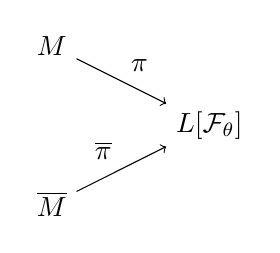
\begin{tikzpicture}
       \node (M) at (0,2) {$M$};
       \node (Mbar) at (0,0) {$\bar{M}$};
       \node (LF) at (2,1) {$L[\mathcal{F}_\theta]$};
       \draw[->] (M) to node[auto]{$\pi$} (LF);
       \draw[->] (Mbar) to node[auto]{$\bar{\pi}$} (LF);
     \end{tikzpicture}
   \end{center}

\marginpar{\tiny{08.01.2013}}

		Setze $B=\{\delta\in \Card\mid \pi(\delta)=\delta\}$ und $\bar B=\{\delta\in\Card\mid \bar\pi(\delta)=\delta\}$.
		Setze $D=C\cap\lambda$.
		Nach Lemma 9 ist $C:= B\cap\bar B$ unbeschränkt in $\On$.
		Wähle $\lambda\in C$ mit $|C\cap\lambda|\ge\kappa^+$.
		Setze $\pi^*=\pi\upharpoonright L_{\lambda}[U]$ und $\bar\pi^* = \bar\pi\upharpoonright L_{\lambda}[\bar U]$.
		Also $\pi^*\colon L_{\lambda}[U]\to L_{\lambda}[\mathcal F_{\theta}$ und $\bar\pi^*\colon L_{\lambda}[\bar U]\to L_{\lambda}[\mathcal F_{\theta}]$ sind elementar.
		Wir zeigen nun die Behauptung.
		Aus Symmetrie genügt z.Z., dass $U\subseteq\bar U$.
		Sei also $X\in U$.
		Nach Lemma 11 gilt, da $X\subseteq\kappa$, $X\in\Hull_{L_{\lambda}[U]}((\kappa+1)\cup D)$, da $|D|\ge\kappa^+$.
		Also existiert Term $t$ und $\vec\lambda<\kappa$, $\vec\rho\in D$ mit $X=t^{L_{\lambda}[U]}(\vec\lambda,\kappa,\vec\rho)$.
		Dann aber $Z:=\pi*(x)=t^{L_{\lambda}[\mathcal F_{\theta}]}(\vec\lambda,\theta, \vec\rho)$, da $\pi*(\vec\gamma,\kappa,\vec\rho)=(\vec\gamma,\theta,\vec\rho)$.
		Also auch $Z\in\rng(\bar\pi^*)$, da $Z=\bar\pi^*(t^{L_{\lambda}[\bar U]}(\vec\gamma,\kappa,\vec\rho)$.
		Also $\bar\pi^*(Z\cap\kappa)=Z$ und $Z\cap\kappa\in\bar U$, da $Z\in\mathcal F_{\theta}$.
		Aber $Z\cap\kappa=X$, da $\pi^*(X)=Z$.

{\bf Korollar:} Sei $\kappa$ meßbar in einem inneren Modell $W$.
	Sei $U\in W$ mit $W\models U$ normaler Ultrafilter auf $\kappa$.
	Dann ist $M=L[U]$ das kleinste innere Modell, in dem $\kappa$ meßbar ist.
	Außerdem ist $U\cap M$ in $M$ der einzige normale Ultrafilter auf $\kappa$.

	{\bf Beweis:} Sei $\bar W$ ein weiteres inneres Modell, in dem $\kappa$ meßbar ist und sei $\bar W\models\bar U$ normaler Ultrafilter auf $\kappa$.
		Nach obigem Satz gilt dann $L[U]=L[\bar U]$, da $L[U]=L[U\cap L[U]]$ und $L[\bar U]=L[\bar U\cap L[\bar U]]$.
		Insbesondere also $L[U]=L[\bar U]\subseteq\bar W$.
		Ist $D\in M$ mit $M\models D$ normaler Ultrafilter auf $\kappa$, so nach Satz ist $D=U\cap M$.

{\bf Satz 13:} Sei $I=\{\kappa\mid\kappa$ ist meßbar in einem inneren Modell $\}$
	Sei $I\neq\emptyset$ und $\kappa=\min I$.
	Sei $M$ das kleinste innere Modell, in dem $\kappa$ messbar.
	Also $M=L[U]$ für ein $U\in M$ mit $L[U]\models U$ normaler Ultrafilter auf $\kappa$.
	Sei $\langle\langle M_i, U_i, \kappa_i\rangle,\pi_{ij}\rangle$ die $\On$-Iteration von $M$ bezüglich $U$.
	Dann gilt $I=\{\kappa_i\mid i\in\On\}$.

	{\bf Beweis:} `'$\supseteq$'' klar. `'$\subseteq$'': Sei $\bar\kappa\in I$. 
		Wegen $\langle\kappa_i\mid i\in\On\rangle$ normal und $\bar\kappa\ge\kappa_0$ existiert dann $i\in\On$ mit $\kappa_i\le\bar\kappa<\kappa_{i+1}$.
		z.Z. $\kappa_i=\bar\kappa$.
		Annahme: $\kappa_i<\bar\kappa$.
		Sei $\bar M=L[\bar U]$ mit $\bar M\neq\bar U$ normaler Ultrafilter auf $\bar\kappa$.
		Sei wieder $\langle\langle \bar M_j,\bar U_j,\bar\kappa_j\rangle,\bar\pi_{jk}\rangle$ die $\On$-Iteration von $\bar M$ bezüglich $\bar U$.
		Wir finden wieder $j\in\On$ mit $\cf(j)>\omega$ und $\kappa_j=\bar\kappa_j=:\theta$.
		Gilt wieder $M_j=L[\mathcal F_{\theta}] = \bar M_j$.
		Setze nun $\pi=\pi{ij}$ und $\bar\pi=\bar\pi_{0j}$.
		Existiert wieder unbeschränktes $C\subseteq\Card$ mit $\pi\upharpoonright C=\id\upharpoonright C=\bar\pi\upharpoonright C$.
		Wähle wieder $\lambda\in C$ mit $|C\cap\lambda|\ge\kappa^+_i$ und setze $D=C\cap\lambda$.
		Wir zeigen nun zuerst \begin{itemize}\item[(*)] Sei $\sigma=\pi_{i,i+1}$. 
		Dann existiert $f\mid\kappa_i\to\kappa_i$, $f\in M_i$, mit $\bar\kappa=\sigma(f)(\kappa_i)$.

		{\bf Beweis von (*):} $\sigma$ ist die Ultrapotenz von $M_i$ mit $U_i$.
			Wegen $\bar\kappa<\kappa_{i+1}=[c{\kappa_i}]$ ist $\bar\kappa=[f]$ für ein $f\colon\kappa_i\to\kappa_i$.
			Wegen $U$ normal ist $[\id\upharpoonright\kappa_i]=\kappa_i$.
			Also $[c_f]([\id\upharpoonright\kappa_i])=[f]$, da $\forall_{\alpha<\kappa_i} c_f(\alpha)(\alpha')=f(\alpha)$.
		\end{itemize}
		
		Setze wieder $\pi^*=\pi\upharpoonright L_{\lambda}[U]$, $\bar\pi^*=\bar\pi\upharpoonright L_{\lambda}[\bar U]$.  Also $\pi^*\colon
                L_{\lambda}[U_i]\to L_{\lambda}[\mathcal F_{\theta}]$, $\bar\pi^*\colon L_{\lambda}[\bar U]\to L_{\lambda}[\mathcal F_{\theta}]$ sind
                elementar.  Sei $f$ wie in $(*)$.  Existiert wieder $\vec\eta<\kappa$ und $\vec\rho\in D$ mit
                $f=t^{L_{\lambda}[U_i]}(\vec\eta,\kappa_i,\vec\rho)$, da $f\subseteq \kappa_i\times\kappa_i$, also im wesentlichen ''$f\in\mathcal
                P(\kappa_i)$''.  Nun ist aber $\pi^*(f)=\pi_{i+1,j}(\pi_{i,i+1}(f))$.  Wegen $\pi_{i+1,j}\upharpoonright\kappa_{i+1}
                =\id\upharpoonright\kappa_{i+1}$ ist also $\pi^*(f)(\kappa_i)=\bar\kappa$.  Aber $\pi^*(f)=t^{L_{\lambda}[\mathcal
                    F_{\theta}]}(\vec\eta,\theta,\vec\rho)\in\rng(\bar\pi^*)$, da $\pi^*(f)=\bar\pi^*(t^{L_{\lambda}[\bar
                    U]}(\vec\eta,\bar\kappa,\vec\rho)$.  Außerdem $\kappa_i\in\rng(\bar\pi^*)$, da $\kappa_i<\bar\kappa=\cp(\bar\pi)$.  Also
                $\bar\kappa=\pi^*(f)(\kappa_i)\in\rng(\bar\pi^*)$.  Widerspruch zu $\bar\kappa=$ kritische Punkt von $\bar\pi^*$.

\marginpar{\tiny{10.01.2013}}

{\bf Satz 14 (Silver):} Sei $V=L[U]$ mit $U$ normaler Filter auf
$\kappa$. Dann gilt $\GCH$.

{\bf Beweis:} Sei $\rho\ge\omega$ Kardinalzahl. Wollen zeigen $2^\rho = \rho^+$.
\begin{itemize}
  \item 1. Fall: $\rho\ge\kappa$. Dann gilt nach Lemma 10 $\mathfrak{P}(\rho)\subseteq L_{\rho^+}[U]$. Also fertig.
  \item 2. Fall: $\rho<\kappa$. Genügt zu zeigen:
    \begin{itemize}
      \item[(*)] Sei $a\subseteq\rho$, $a\in L_{\gamma+1}[U]\backslash L_\gamma[U]$. Dann ist $|\mathfrak{P}(\rho)\cap L_{\gamma+1}[U]|\le\rho$.
      \item[] {\bf Beweis:} Sei $\Theta>\gamma$, $2^\kappa$ regulär. Setze $\mathfrak{A}=\left<L_\Theta[U], \in, U, \{a\},
        (\alpha)_{\alpha\le\rho}\right>$. Zeige zuerst:
        \begin{itemize}
          \item[(1)] existiert $I\in U$ mit $I$ ist Menge von Indiscernibles für $\mathfrak{A}$
          \item[] {\bf Beweis:} (Analog zu Lemma 2 aus §2:) Sei $\mathcal{L}$ die zu $\mathfrak{A}$ gehörige Sprache. Definiere
            $f:[\kappa]^{<\omega}\rightarrow \mathfrak{P}(\Form_{\mathcal{L}})$ durch $f(\{v_0, \ldots, v_{n-1}\})=\tp_{\mathfrak{A}}(\left<v_0,
            \ldots, v_{n-1}\right>)$. Nach Satz 3 existiert $I\in U$ mit $I$ homogen für $f$. $I$ ist wie gewünscht. \hfill $\square$
        \end{itemize}
        Sei also $I$ wie in (1). Setze $\mathcal{H} = \Hull_{\mathfrak{A}}(I)$. Sei $\sigma:\mathcal{H}\xrightarrow{\sim}\left< L_\delta[\bar{U}],
        \in, \bar{U}, \ldots\right>$. Gilt $\sigma\upharpoonright(\rho+1)=\id\upharpoonright(\rho+1)$, $\sigma(a)=a$.
        \begin{itemize}
          \item[(2)] es existiert $X\in U$ mit $\rho\upharpoonright X = \id\upharpoonright X$ (insbesondere $X\subseteq\mathcal{H}$)
          \item[] {\bf Beweis:} Angenommen nicht. Beachte, dass für alle $\beta\in\mathcal{H}$ gilt $\sigma(\beta)\le\beta$. Nach Annahme ist also
            $Z=\{\beta\in I\mid\rho(\beta)<\beta\}\in U$. Dann existiert wegen $U$ normal ein $\mu<\kappa$ mit $\bar{Z}=\{\beta\in I\mid
            \sigma(\beta)=\mu\}\in U$. Widerspruch zu $\sigma$ injektiv. \hfill $\square$
          \item[(3)] $L_\delta[\bar{U}] = L_\delta[U]$.
          \item[] {\bf Beweis:} Es ist $\bar{U} = \sigma''(\mathcal{H}\cap U)$. Also genügt es zu zeigen, dass $\sigma''(\mathcal{H}\cap U)=U\cap
            L_\delta[\bar{U}]$. Genügt zu zeigen ``$\subseteq$'', da beide Seiten Ultrafilter auf $\mathfrak{P}(\kappa)\cap L_\delta[\bar{U}]$
            sind. Sei hierzu $X$ wie in (2). Dann gilt für $Z\in\mathcal{H}\cap U$
            $$ \sigma(Z) = \sigma''(Z\cap\mathcal{H}) \supseteq \sigma''(Z\cap X) = Z\cap X\in U $$ Also $\sigma(Z)\in U$. \hfill $\square$
        \end{itemize}
        Wegen $a=\sigma(a)\in L_\delta[\bar{U}]$, also nach (3) $a\in L_\delta[U]$. Somit $\delta\ge\gamma+1$. Genügt also zu zeigen
        $|\mathfrak{P}(\rho)\cap L_\delta[U]|\le\rho$. Hierzu zeigen wir
        \begin{itemize}
          \item[(4)] $\mathfrak{P}(\rho)\cap\mathcal{H}\subseteq\Hull_{\mathfrak{A}}(\bar{I})$, wobei $\bar{I}$ die ersten $\omega$ Elemente von $I$
          \item[] {\bf Beweis:} Sei $b\in\mathfrak{P}(\rho)\cap\mathcal{H}$. Dann existiert $\delta_0,\ldots,\delta_{n-1}\in I$ und Term $t$ mit
            $b=t^{\mathcal{H}}(\delta_0,\ldots,\delta_{n-1})$. Seien nun $\gamma_0,\ldots,\gamma_{n-1}$ die ersten $n$ Elemente von $I$. Dann gilt
            auch $b=t^{\mathcal{H}}(\gamma_0,\ldots,\gamma_{n-1})$, denn für $\alpha<\rho$ $\mathfrak{A}\models\alpha\in
            t^{\mathcal{H}}(\gamma_0,\ldots,\gamma_{n-1})\leftrightarrow \alpha\in t^{\mathcal{H}}(\delta_0,\ldots,\delta_{n-1})$ und
            $t^{\mathcal{H}}(\gamma_0,\ldots,\gamma_{n-1})\subseteq\rho$ \hfill $\square$
        \end{itemize}
    \end{itemize}
\end{itemize}

{\bf Satz 15:} Sei $U$ ein $\kappa$-vollständiger Ultrafilter auf $\kappa$. Sei $j:V\rightarrow M$, $M$ transitiv, die Ultrapotenzabbildung mit
$U$. Dann gilt $U\not\in M$.

{\bf Beweis:} $F=\{f\mid f:\kappa\rightarrow\kappa\}$. Dann gilt $\otp(\left<F,<_u\right>)=j(k)$ wobei $f<_u g \Leftrightarrow \{\alpha<\kappa\mid
f(\alpha)< g(\alpha)\}\in U$. Nun ist aber $F\in M$, da $\mathfrak{P}(\kappa)\subseteq M$. Angenommen $U\in M$. Dann ist auch $<_u\in M$, also
$\left<F,<_\kappa\right>\in M$. Also in $M$ $j(\kappa)=\otp(\left<F,<_u\right>)<(2^\kappa)^+$, da $|F|=2^\kappa$. Also $j(\kappa)$ ist unerreichbar in
$M$, da $\kappa$ unerreichbar in $V$. Widerspruch.

{\bf Folgerung:} Sei $\left< \left<M_i, U_i, \kappa_i\right>, \pi_{ij}\right>$ die $\On$-Iteration von $M$ bezüglich $U$. Dann gilt
$$ M_o \supsetneq M_1 \supsetneq M_2 \supsetneq \ldots \supsetneq M_i $$

{\bf Satz 16:} Sei $V=L[U]$ mit $U$ normaler Ultrafilter auf $\kappa$. Dann ist $\kappa$ die einzige messbare Kardinalzahl.

{\bf Beweis:}
\begin{itemize}
  \item 1. Fall: $\tau > \kappa$. Sei $D$ ein $\tau$-vollständiger Ultrafilter auf $\tau$ und $j:V\rightarrow M$ die Ultrapotenzabbildung mit
    $D$. Dann gilt wegen $\tau>\kappa$ auch $j(U)=U$, als $M=L[j(U)]=L[U]=V$. Widerspruch zu Satz 15, da $D\not\in M$.
  \item 2. Fall: $\tau < \kappa$. Sei $N$ das kleinste innere Model, in dem $\tau$ messbar ist. Dann ist nach Satz 15 $V$ eine Iteration von $N$. Also
    nach obiger Folgerung ist $V\subsetneq N$. Widerspruch.
\end{itemize}
 \hfill $\square$

$j:V\rightarrow M$ Ultrapotenz mit $U$ auf $\kappa$, $U\not\in M$, das heißt $\mathfrak{P}(\mathfrak{P}(\kappa))\not\subseteq M$.

\marginpar{\tiny{15.01.2013}}

\section{Sehr große Kardinalzahlen}
Für eine Kardinalzahl $\kappa$ setze $$H_\kappa=\{x\mid |\TC(x)|<\kappa\}$$ wobei $\TC(x)$ die transitive Hülle von $x$ ist. Natürlich gilt
$\kappa<\lambda\Rightarrow H_\kappa\subseteq H_\lambda$, $\kappa$ Limeskardinalzahl $\Rightarrow$ $H_\kappa = \bigcup\limits_{\lambda<\kappa}
H_\lambda$, $V=\bigcup\limits_\kappa H_\kappa$.

{\bf Satz 1:} Sei $j:H_\kappa\rightarrow M$ elementar mit $M$ transitiv. Weiterhin sei $\cf(\kappa)>\omega$. Dann existeren transitives $N$ und
$j^*:V\rightarrow N$ elementar mit $j^*\supseteq j$.

{\bf Beweis:} Setze $$Q = \{\left<f, a\right>\mid \mbox{es existiert }u\in H_\kappa\mbox{ mit }f:u\rightarrow V\mbox{ und }a\in j(u)\}$$ Definiere
eine Relation $\sim$ auf $Q$ durch: $$ \left<f, a\right>\sim\left<g,b\right> \Leftrightarrow \left<a,b\right>\in j(\{\left<c,d\right>\mid
f(c)=g(d)\}) $$ $\sim$ ist Äquivalenzrelation, denn:
\begin{itemize}
  \item $\left<f,a\right>\sim\left<f,a\right>$, denn: $j(\{\left<c,d\right>\mid f(c)=g(d)\})\supseteq\{\left<e,e\right>\mid e\in\dom
    j(f)\}\ni\left<a,a\right>$.
  \item Symmetrie ist klar, denn $\left<a,b\right>\in j(\{\left<c,d\right>\mid f(c) = g(d)\}) \rightarrow \left<b,a\right>\in j(\{\left<d,c\right>\mid
    g(d)=f(c)\})$.
  \item Transitiv: $\left<a,b\right>\in j(\{\left<c,d\right>\mid f(c)=g(d)\})$ und $\left<b, e\right>\in j(\{\left<d,i\right>\mid
    g(d)=h(i)\})\rightarrow \left<c,i\right>\mid f(c) = h(i)\}$
\end{itemize}
Für $\left<f,a\right>\in Q$ setze $$ [f,a] = \{ \left<g, b\right> \mid \left<f, a\right>\sim\left<g,b\right> \mbox{ und für alle } \left<h,c\right>
\mbox{ mit } \left<f,a\right>\sim\left<h,c\right> \mbox{ ist } \rng(g)\le\rng(h)\} $$ Sei $\tilde{Q} = \{[f,a]\mid\left<f,a\right>\in Q\}$. Definiere
eine Relation $E$ auf $\tilde{Q}$ durch $[f,a] E [g,b] \Leftrightarrow \left<a,b\right>\in j(\{\left<c,d\right>\mid f(c)\in g(d)\})$. Dies ist
wohldefiniert.

Wir zeigen nun:
\begin{itemize}
  \item[(1)] Sei $\varphi(x_1,\ldots,x_n)$ eine Formel. Dann: $\left<\tilde{Q},E\right>\models\varphi([f_1,a_1],\ldots,[f_n,a_n]) \Leftrightarrow
    \left<a_1,\ldots,a_n\right>\in j(\{\left<c_1,\ldots,c_n\right>\mid H_\kappa\models\varphi(f_1(c_1),\ldots,f_n(c_n))\})$.
  \item[] {\bf Beweis:} Durch Induktion über den Formelaufbau:
    \begin{itemize}
      \item[(a)] $\varphi$ atomar \\ nach Def.
      \item[(b)] $\varphi \equiv \varphi_1 \vee \varphi_2$ \\ da $j(A\cup B) = j(A) \cup j(B)$, für $A,B\in H_\kappa$
      \item[(c)] $\varphi \equiv \lnot \psi$ \\ da $j(U\backslash A) = j(U)\backslash j(A)$, für $A, U\in H_\kappa$
      \item[(d)] $\varphi \equiv \exists_z \psi(z,x_1,\ldots,x_n)$
        \begin{itemize}
          \item[``$\Rightarrow$''] Sei $\left<\tilde{Q},E\right>\models \psi([g,b],[f_1,a_1],\ldots,[f_n,a_n])$. Setze $A =
            \{\left<c,c_1,\ldots,c_n\right>\mid H_\kappa \models \psi(g(c),f_1(c_1),\ldots,f_n(c_n))\}$. Nach Induktionsvoraussetzung
            $\left<b,a_1,\ldots,a_n\right>\in j(A)$. Setze $D=\{\left<c_1,\ldots,c_n\right>\mid
            H_\kappa\models\varphi(f_1(c_1),\ldots,f_n(c_n))\}$. Dann gilt für alle $\left<c,c_1,\ldots,c_n\right>\in A$ dass
            $\left<c_1,\ldots,c_n\right>\in D$. Dies überträgt sich auf $j(A),j(D)$. Wegen $\left<b,a_1,\ldots,a_n\right>\in j(A)$ also
            $\left<a_1,\ldots,a_n\right>\in j(D)$. \hfill $\square$
          \item[``$\Leftarrow$''] Setze wieder $D=\{\left<c_1,\ldots,c_n\right>\mid H_\kappa\models\varphi(f_1(c_1),\ldots,f_n(c_n))\}$. Sei
            $\dom(f_i)=u_i$. Definiere $g:u_1\times\ldots\times u_n \rightarrow V$ so, dass gilt:
            $H_\kappa\models\varphi(f_1(c_1),\ldots,f_n(c_n))\rightarrow H_\kappa\models\psi(g(c_1,\ldots,c_n),f_1(c_1),\ldots,f_n(c_n))$. Setze nun
            $A = \{\left<c,c_1,\ldots,c_n\right>\mid H_\kappa\models\psi(g(c),f_1(c_1),\ldots,f_n(c_n))\}$ und $b = \left<a_1,\ldots,a_n\right>$. Also
            $b\in j(u_1\times\ldots\times u_n)$. Es gilt: $$ \left<c_1,\ldots,c_n\right>\in D\rightarrow
            \left<\left<c_1,\ldots,c_n\right>,c_1,\ldots,c_n\right>\in A$$ Dies überträgt sich auf $j(D)$ und $j(A)$. Somit erhalten wir: Ist
            $\left<c_1,\ldots,c_n\right>\in j(D)$, so ist $\left<b,a_1,\ldots,a_n\right>\in j(A)$. Also nach Induktionsvoraussetzung
            $\left<\tilde{Q},E\right>\models\psi([g,b],[f_1,a_1],\ldots,[f_n,a_n])$ und daher
            $\left<\tilde{Q},E\right>\models\varphi([f_1,a_1],\ldots,[f_n,a_n])$. \hfill $\square$(1)
        \end{itemize}
    \end{itemize}
  \item[] Für $x\in V$ definiere $c_x:1\rightarrow V$ durch $c_x(0)=x$. Definiere nun $\tilde(j):V\rightarrow\tilde{Q}$ durch
    $\tilde{j}(x)=[c_x,0]$. Aus (1) folgt sofort:
  \item[(2)] $\tilde{j}:V\rightarrow\left<\tilde{Q},E\right>$
  \item[] Wir zeigen nun:
  \item[(3)] $E$ ist stark fundiert.
  \item[] {\bf Beweis ``stark'':} Sei $[g,b]\in\tilde{Q}$. Sei $v=\bigcup\limits_{d\in\dom(g)}g(d)$ und sei $z\not\in v$ fest. Ist nun $[f,a]E[g,b]$,
    so definiere $f^*:\dom(f)\rightarrow V$ durch $$ f^*(c) = \left\{ \begin{array}{cl} f(c) & \mbox{falls } f(c)\in v \\ z &
      \mbox{sonst}\end{array}\right.$$ Dann ist $[f,a]\sim[f^*,a]$, denn: $a\in j(\{c\mid\exists_d . f(c)\in g(d)\}) = j(\{c\mid f(c)=f^*(c)\})$. Also
    ist $\{[f,a]\mid [f,a]E[g,b]\}\in V$, da $\{f^*\mid\ldots\}$ eine Menge ist.
%\end{itemize}

\marginpar{\tiny{17.01.2013}}

%$[f,a]$ ist modifizierte Äquivalenzrelation.
%$\tilde Q:=\{[f,a]\mid\langle f,a\rangle\in Q\}$ und $[f,a]E[g,b]\iff \langle a,b\rangle\in j(\{\langle c,d\rangle\mid f(c)\in g(d)\})$.
%Für $x\in V$ definiere $c_x\colon 1\to V$ durch $c_x(0)=x$.
%Definiere nun $\tilde j\colon V\to\tilde Q$ durch $\tilde j(x)=[c_x,0]$.
%Denn $\tilde j\colon V\to\langle \tilde Q,E\rangle$ elementar.
%\begin{itemize}\item[(3)] $E$ ist stark fundiert
	\item[] {\bf Beweis ``fundiert'':} Ann.: $E$ ist nicht fundiert.
		Sei also $[f_{n+1},a_{n+1}E[f_n,a_n]$ für alle $n$.
		Sei $\{f_n\mid n\in \omega\}\subseteq H_{\lambda}$ für ein $\lambda$.
		Setze $u=\bigcup_n\dom(f_n)$.
		Dann ist $n\in H_{\kappa}$, da $\cf(\kappa)>\omega$ und für alle $n$ $\dom(f_n)\in H_{\kappa}$.
		Wähle ein $X\prec H_\lambda$ mit $TC(u)\cup\{f_n\mid n\in\omega\}\subseteq X$ und $|X|<\kappa$.
		Sei $\pi\colon X\tilde\to R$ mit $R$ transitiv.
		Also $R\in H_{\kappa}$.
		Setze $g_n=\pi(f_n)$.
		Weiterhin sei $A_n=\{\langle c,d\rangle\mid f_{n+1}(c)\in f_n(d)\}$.
		Es ist dann $A_n\subseteq u\times u$.
		Wegen $\pi\upharpoonright TC(u)=\id\upharpoonright u$ ist dann $\pi(A_n)=A_n$.
		Aber $\pi(A_n)=\{\langle c,d\rangle\mid g_{n+1}(c)\in g_n(d)\}$.
		Wegen $[f_{n+1},a_{n+1}]E[f_n,a_n]$ ist aber dann $\langle a_{n+1},a_n\rangle\in j(A_n)=j(\{\langle c,d\rangle\mid g_{n+1}(c)\in g_n(d)\})=$
		$\{\langle c,d\rangle\mid j(g_{n+1}(c)\in j(g_n)(d)\}$, d.h. $j(g_{n+1}(a_{n+1})\in j(g_n))(a_n)\;\forall_n$. Wid.
\end{itemize}
Sei also $\pi\colon\langle \tilde Q,E\rangle\tilde\to N$ mit $N$ transitiv.
Definiere $j^*\colon V\to N$ durch $j^*=\pi\circ\tilde j$.
Dann ist $j^*$ elementar.
Wir müssen zeigen:
\begin{itemize}\item[(4)] $j^*\supseteq j$

		{\bf Beweis:} Setze $M'=\bigcup_{n\in H_\kappa}j(n)$.
		Definiere eine Abbildung $\sigma\colon M'\to N$ wie folgt.
		Sei $a\in M'$.
		Wähle $u\in H_{\kappa}$ mit $a\in j(u)$
		und setze $\sigma(a)=\pi([\id\upharpoonright u, a])$.
		Dies hängt nicht von der Wahl von $u$ ab.
		Setze $N'=\rng(\sigma)$.
		Man sieht leicht, das $\sigma\colon M'\to N'$ ein Isomorphismus ist.
		Aber $N'$ ist transitiv.
		Denn sei $[f,b]E[\id\upharpoonright u,a]$, wobei o.E. $u$ transitiv.
		Wie im Beweis von (3) dann o.E. $f\in H_\kappa$.
		Dann aber $\langle f,b\rangle\sim\langle \id\upharpoonright u, j(f)(b)\rangle$, woraus das Gewünscht folgt.
		Somit ist $\sigma$ die Identität.
		Aber für $x\in H_\kappa$ ist $\tilde j(x)=[c_x,0] \stackrel{!}{=}[\id\upharpoonright\{x\}, j(x)]$
		also $j^*(x)=\sigma(j(x))=j(x)$.
		$j^*(x)=\pi(\tilde j(x))=\sigma(j(x))=j(x)$.
\end{itemize}

{\bf Definition:} Sei $j\colon V \to M$ elementar mit M transitiv, und sei $j\neq\id$.
	Setze dann $\cp(j)=\min\{\kappa\mid j(\kappa)\neq\kappa\}$ der {\em kritische Punkt} von $j$.

{\bf Definition:} \begin{itemize}\item[(a)] Seien $\kappa,\lambda$ Kardinalzahlen.
		$\kappa$ ist {\em $\lambda$-stark} $\iff$ es existiert $j\colon V\to M$ elementar mit $M$ transitiv, $\kappa=\cp(j)$, $\lambda<j(\kappa)$ und $\mathcal P(\lambda)\subseteq M$.
		\item[(b)] $\kappa$ ist {\em stark}, wenn $\kappa$ $\lambda$-stark für alle $\lambda$ ist.
	\end{itemize}

{\bf Bemerkung:} Nach Satz 1 lässt sich ``$\kappa$ ist $\lambda$-stark'' in $\ZFC$ definieren, denn es gilt:
	$\kappa$ ist $\lambda$-stark $\iff$ es existiert $\lambda\colon j(\kappa)$ und $\mathcal P(\lambda)\subseteq N$.

{\bf Bemerkung:} $\kappa$ ist $0$-stark $\iff$ $\kappa$ ist $\kappa$–stark $\iff$ $\kappa$ ist messbar.

{\bf Bemerkung:} Sei $M$ ein inneres Modell und $\mathcal P(\lambda)\subseteq M$.
	Dann gilt $H_{\lambda^+}\subseteq M$.
	
	{\bf Beweis:} Da in $M$ eine Bijektion von $\lambda$ nach $\lambda\times\lambda$ existiert ist $\mathcal P(\lambda\times\lambda)\subseteq M$.
		Sei nun $x\in H_{\lambda^+}$, und sei $z=\TC(x)$.
		Also $|z|\le\lambda$.
		Sei $f\colon\alpha\to z$ Bijektion mit $\alpha=|z|$ und definiere $E\subseteq \alpha\times\alpha$ so, dass $f\colon\langle\alpha, E\rangle\to\langle z,\in\rangle$ en Isomorphismus ist.
		Somit ist $f$ die Transitivierung von $\langle \alpha, E\rangle$.
		Wegen $E\subseteq\lambda\times\lambda$ ist also $\langle\alpha, E\rangle\in M$.
		Somit ist aber auch $f\in M$, da $M$ inneres Modell.
		Sei non $y={f^{-1}}''x$.
		Also $y\in M$, da $y\subseteq \lambda$.
		Somit $x=f''y\in M$.

{\bf Satz 2:} Sei $\kappa$ $2^\kappa$-stark.
	Dann existiert normaler Ultrafilter $U$ auf $\kappa$ mit $\{\alpha<\kappa\mid \alpha \mbox{ messbar}\}\in U$.

	{	\bf Beweis:} Sei $j\colon V\to M$ wie in Def. von ``$\kappa$ ist $2^\kappa$-stark''.	
	Setze $U=\{X\in \kappa\mid \kappa\in j(X)\}$.
	Dann ist $U$ normaler Ultrafilter auf $\kappa$ (siehe früher).
	Aber $U\in \mathcal P(\mathcal P(\kappa))\subseteq H_{(2^\kappa)^+}$.
	Wegen $\mathcal P(2^\kappa)\subseteq M$ ist also nach Bem. $U\in M$.
	Somit $M\models \kappa \mbox{ ist messbar}$.
	Somit nach Def. von $U$ ist $X=\{\alpha<\kappa\mid \alpha \mbox{ is messbar}\}\in U$, da $\kappa\in j(X)$.

{\bf Bemerkung:} Sei $\kappa$ $\lambda$-stark, wobei $\lambda\ge\kappa$.
	Dann existieren transitives $N$ und $j\colon H_{\kappa^+}\to N$ elementar mit $\kappa=\cp(j)$, $\lambda<j(\kappa)$, $\mathcal(\lambda)\subseteq N$ und $|N|\le 2^\lambda$.

	{\bf Beweis:} Sei $k \colon H_{\kappa^+}\to M$ elementar mit $M$ transitiv.
		$\kappa=\cp(j)$, $\lambda<k(\kappa)$, $\mathcal P(\lambda)\subseteq M$.
		Sei $X\prec N$ mit $\rng(k)\cup\mathcal P(\lambda)\subseteq X$ und $|X|\le 2^\lambda$.
		Sei $\pi\colon X\to N$ die Transitivierung von $X$.
		Setze $j=\pi\circ k$.
		Dann ist $j$ wie gewünscht.

\marginpar{\tiny{22.01.2013}}

{\bf Bemerkung:} $\kappa$ ist stark $\to$ $\kappa$ ist total unbeschreibbar

	{\bf Beweis:} Sei $A\subseteq V_\kappa$ und $\gamma >\kappa$ mit $V_{\gamma}\models\varphi(A)$.
		Wegen $\kappa$ stark existiert $j\colon V\to M$ elementar, $M$ transitiv, mit $\cp(j)=\kappa$, $j(\kappa)>\gamma$ und $V_\gamma\subseteq M$.
		Denn $V_{j(\gamma)}^M\models \varphi(j(A))$.
		Aber $M\models \exists_\alpha\exists_\delta\left(\alpha<\delta<j(\kappa) \mbox{ und } V_{\delta}\models \varphi(j(A)\cap V_{\alpha})\right)$
		nämlich $\alpha=\kappa$ und $\delta=\gamma$, da $j(A)\cap V_{\kappa}=A$ und $V^M_{\gamma}=V_\gamma$.
		Also $V\models\exists_\alpha\exists_\delta\left( \alpha<\delta<\kappa \mbox{ und } V_{\delta}\models\varphi(A\cap V_{\alpha})\right)$.

{\bf Definition:} $\kappa$ ist {\em Woodin} $:\iff$ für alle $f\colon\kappa\to\kappa$ existiert $\tau<\kappa$ mit $f''\tau \subseteq \tau$ und ein elementares $j\colon V\to M$ mit $M$ transitiv, $cp(j)=\tau$ und $V_{j(f)(\tau)}\subseteq M$.

{\bf Bemerkung:} Sei $\kappa$ Woodin.
	Dann ist $\{ \tau<\kappa\mid  \tau$ messbar $\}$ stationär in $\kappa$.
	Insbesondere ist $\kappa$ Mahlo.

	{\bf Beweis:} Sei $C\subseteq\kappa$ abgeschlossen unbeschränkt. 
		Definiere $f\colon \kappa\to\kappa$ durch $f(\alpha) = \min (C-(\alpha+1))$.
		Sei $\tau$ wie in Definition, dann $f''\tau\subseteq\tau$, also $\tau$ Limespunkt von $C$, also $\tau\in C$ und wegen Existenz von $j$ ist $\tau$ messbar.

{\bf Satz 3:} Sei $\kappa$ Woodin.
	Dann existiert $\tau<\kappa$ mit $V_\kappa\models\tau$ ist stark.

	{\bf Beweis:} Annahme: nicht.
		Definiere also $g\colon\kappa\to\kappa$ so, dass für alle $\tau<\kappa$ $V_{\kappa}\models\tau$ ist nicht $g(\tau)$-stark, und $g(\tau)\ge\tau$.
		Nach obiger Bemerkung gilt dann wirklich, dass $\tau$ nicht $g(\tau)$-stark.
		Definiere nun $f\colon\kappa\to\kappa$ durch $f(\tau)=$ die kleinste unerreichbare Kardinalzahl $>g(\tau)$.
		Wegen $\kappa$ Woodin existiert $\tau<\kappa$ und ein elementares $j\colon V\to M$ mit $M$ transitiv, $cp(j)=\tau$ und $V_{j(f)(\tau)}\subseteq M$, also 
		$M\models \exists \beta<j(f)(\tau)$ $\tau$ ist nicht $\beta$-stark.
		Wegen $V_{j(f)(\tau)}\subseteq M$ ist dann $\tau$ wirklich nicht $\beta$-stark für ein $\beta< j(f)(\tau)$.
		Wegen $\mathcal P(\beta)\subseteq V_{j(f)(\tau)}\subseteq M$ ist dies aber ein Wiederspruch zur Existenz von $j$.

{\bf Definition:} Sei $A$ eine Klasse.
	$\kappa$ ist stark bezüglich $A$, wenn für alle $\gamma$ ein $j\colon V\to M$ elementar existiert mit $M$ transitiv, $\kappa=\cp(j)$, $\gamma<j(\kappa)$, $v_{\gamma}\subseteq M$ und $A\cap V_{\gamma}= j(A)\cap V_{\gamma}$
	[wobei: $j(A)=\bigcup \{j(A\cap x)\mid x\in V\}$]

{\bf Bemerkung:} Wie früher zeigt man: Ist $\kappa$ stark bezüglich $A$, so existiert für alle $\gamma$ ein $j\colon H_{\kappa^+}\to N$ mit $N$ transitiv, $\kappa=\cp(j)$, $\gamma<j(\kappa)$, $V_{\gamma}\subseteq M$, $A\cap V_\gamma= j(A)\cap V_\gamma$ und $|N|=|V_\gamma|$.

{\bf Satz 4:} Es sind äquivalent:
	\begin{itemize}
		\item[(1)] $\kappa$ ist Woodin
		\item[(2)] ($\kappa$ ist unerreichbar und) für alle $A\subseteq V_{\kappa}$ ist $\{\tau<\kappa\mid V_{\kappa}\models \tau \mbox{ ist stark bezüglich } A\}$ stationär in $\kappa$.
		\item[(3)] $\kappa$ ist unerreichbar und für alle $A\subseteq V_{\kappa}$ existiert $\tau<\kappa$ mit $V_{\kappa}\models \tau$ ist stark bezüglich $A$
	\end{itemize}

\marginpar{\tiny{24.01.13}}
	{\bf Beweis:}\begin{itemize}\item (1)$\to$(2): Sei $A\subseteq V_\kappa$ und setze $E=\{\tau<\kappa\mid V_\kappa\models \tau \mbox{ ist stark bezüglich } A\}$.
		Sei $C\subseteq \kappa$ abgeschlossen unbeschränkt in $\kappa$.
		Z.Z. $C\cap E\neq\emptyset$.
		Definiere hierzu $g\colon\kappa\to\kappa$ wie folgt:
		Sei $\tau<\kappa$.
		Gilt $V_{\kappa}\models \tau$ ist stark bezüglich $A$, so sei $g(\tau)=0$.
		Ist die nicht der Fall, so wähle $\gamma<\kappa$ minimal, so dass in $V_{\kappa}$ kein $j\colon H_{\kappa^+}\to N$ mit $N$ transitiv, $\kappa=\cp(j)$,
		$\gamma<j(\kappa)$, $A\cap V_{\gamma}=j(A)\cap V_\gamma$ existiert.
		Setze $g(\tau)=\gamma$.
		Definiere nun $f\colon \kappa\to\kappa$ durch $f(\tau)=\max\{g(\tau)+2, \min(C-(\tau+1))\}$.
		Nach (1) existiert dann $\tau<\kappa$ und mit $f''\tau\subseteq\tau$ und ein elementares $j\colon V\to M$ mit $M$ transitiv, $\cp(j)=\tau$ und $V_{j(f)(\tau)}\subseteq M$.
		Wegen $f''\tau\subseteq\tau$ ist dann Limespunkt von $C$, also $\tau\in C$.
		Somit auch $\tau \in j(C)$, da $C\cap\tau \subseteq j(C)$.
		Somit genügt z.Z., dass $\tau\in j(E)$.
		Nehme an, dass dies nicht der Fall ist und setze $\gamma= j(g)(\tau)$.
		Dann existiert also in $j(V_\kappa)$ kein  $k\colon H_{\tau^+}\to N$ min $N$ transitiv, $\tau=\cp(k)$, $\gamma<k(\tau)$, $V_\gamma\subseteq N$, $j(A)\cap V_\gamma = k(j(A))\cap V_\gamma$.
		Setze nun $j^*=j\upharpoonright H_{\tau^+}$, $N=j(H_{\tau^+})$.
		Also $j^*\colon H_{\tau^+}\to N$ elementar, $N$ transitiv.
		Weiterhin ist $V_{\gamma}\subseteq N$ und $j^*(j(A))\cap V_\gamma=j^*(j(A)\cap H_{\tau})\cap V_{\gamma}=j^*(A\cap H_\tau)\cap V_\gamma =  j^*(A)\cap V_{\gamma}$
		Dann existiert aber auch solch ein $k$, $\tilde N$ mit $|\tilde N|\le V_\gamma$.
		Dann ist aber $k\in M$, also $k\in j(V_\kappa)$, was ein Widerspruch ist.
		\item (2)$\to$(3): ist trivial.
		\item (3)$\to$(1): Sei $f\colon\kappa\to\kappa$.
		Wähle gemäß (3) ein $\tau<\kappa$ mit $V_\kappa\models\tau$ stark bezüglich $f$.
		Wegen $\kappa$ regulär existiert $\tau<\beta<\kappa$ mit $f''(\tau+1)\subseteq\beta$.
		Wähle dann ein $j\colon V_{\kappa}\to M$ elementar mit $M$ transitiv, $\tau = \cp(j)$, $\beta< j(\tau)$, $V_{\beta}\subseteq M$ und $f\cap V_{\beta}=j(f)\cap V_{\beta}$.
		Für $\alpha<\tau$ ist dann $\langle \alpha, f(\alpha)\rangle\in f\cap V_{\beta}$.
		$j(f)(\alpha)=f(\alpha)$.
		Somit $f(\alpha)<\tau$, da sonst $j(f(\alpha))\ge j(\tau) > \beta\ge f(\alpha)$.
		Also $f''\tau\subseteq\tau$.
		Weiterhin ist $\langle\tau, f(\tau)\rangle\in f\cap V_{\beta} = j(f)\cap V_{\beta}$.
		Also $j(f)(\tau)=f(\tau)$.
		Wegen $f(\tau)\le\beta$.
		Also $V_{j(f)(\tau)}\subseteq V_\beta\subseteq M$.
		Dies war zu zeigen.
	\end{itemize}

{\bf Definition:} $\kappa$ ist {\em superstark} :gdw es existiert $j\colon V\to M$ elementar mit $M$ transitiv, $\kappa=\cp(j)$ und $V_{j(\kappa)}\subseteq M$.

{\bf Satz 5:} Sei $\kappa$ superstark.
	Dann ist $\kappa$ Woodin.
	Es existiert $\tau<\kappa$ mit $\tau$ ist Woodin.

	{\bf Beweis:} Sei $f\colon \kappa\to\kappa$.
		Wähle $j\colon V\to M$ elementar mit $M$ transitiv, $k=\cp(j)$ und $V_{j(\kappa)}\subseteq M$.
		Somit gilt insbesondere $V_{j(f)(\kappa)}\subseteq M$, da $j(f)(\kappa)<j(\kappa)$.
		Mit dem üblichen Argument existiert dann $k\in V_{j(\kappa)}$ und transitives $N\in V_{j(\kappa)}$ mit $k\colon H_{\kappa^+}\to N$ elementar und $V_{k(f)(\kappa)}\subseteq N$.
		Also $M\models$ es existiert $\tau< j(\kappa)$ mit $j(f)''\tau\subseteq\tau$ und $\pi\colon H_{\tau^+}\to R$ elementar mit $R$ transitiv, 
		$\cp(\pi)=\tau$ und $V_{\pi(f)(\tau)}\subseteq R$, nämlich $\tau=\kappa$.
		Somit $V\models\ldots$.

Sei weiterhin $j,M$ wie oben. Dann $M\models\kappa$ ist Woodin. Also existiert $\tau<\kappa$ mit $\tau$ ist Woodin.

{\bf Definition:} $\kappa$ ist {\em subkompakt} :gdw für alle $B\subseteq H_{\kappa^+}$ existieren $\tau<\kappa$, $A\subseteq H_{\tau^+}$ und elementare Einbettung $j\colon\langle H_{\tau^+}, A\rangle\to\langle H_{\kappa^+}, B\rangle$ mit $\cp(j)=\tau$.

{\bf Bemerkung:}	Ist $\kappa$ subkompakt, so ist $\kappa$ unerreichbar 
	(denn oben: $\tau$ unerreichbar (sogar messbar), also $\kappa$ unerreichbar, da $j(\tau)=\kappa$.)

{\bf Satz 6:} Sei $\kappa$ subkompakt.
	Dann $V_{\kappa}\models$ es existiert $\gamma$ mit $\gamma$ ist superstark
	(also existiert $\gamma<\kappa$ mit $\gamma$ ist superstark).

































\end{document}
